%%%
%%%
%%% Main TeX File for Lecture Stochastic Simulations in Physics 
%%%
%%%   SS 1998  PD Dr. F. Petruccione  
%%%
%%%
%%% (LaTeX2e Code: P. Biechele) 
%%%
%%%
\documentclass[fleqn,10pt,a4paper,openright]{book}
\NeedsTeXFormat{LaTeX2e}[1996/06/01]
%
% Options:  fleqn     Formulas left not centered
%           leqno     formula numbers to the left, not right
%           openright ????
%
% Create Index
%\usepackage{makeidx}
%\makeindex
%%% English Hyphenations and Titles
\usepackage[german,english]{babel}

%%% USE POSTSCRIPT FONTS (NOT TeX Fonts)
\usepackage{times,helvet,mathptm}

%%% AMS LaTeX Extensions + Fonts 
\usepackage{amssymb}
\usepackage[centertags,intlimits,namelimits,sumlimits,reqno]{amsmath}

%%%%%%%  The graphicx/color style for picture inclusion and color support
\usepackage[dvips]{graphicx,color}
% set path for figures
% more directories can be added by using {dir/} for each
\graphicspath{ {Figures/} }

%%% The Listings package - include source code
\usepackage{listings}
% standard listing gormatting
\selectlisting{matlab}
% line numbers ? And what stepsize ?
\labelstyle[1]{\ttfamily}
% use small font size for typesetting listings
\prelisting{\small\smallskip\hrule\smallskip}
\postlisting{\smallskip\hrule\smallskip}


% Use extended theorem style
\usepackage{theorem}

%%% The Chapterbib package for Bibliographies per chapter
% TeX usage:  Just insert \bibliography{...bib} where you want to have a bib
%             The style can be given for each bib, but NOT in the main file !
% Compile usage: latex mainfile
%                bibtex chap1
%                bibtex chap2     etc.  (for each chapter)
%                latex mainfile    ! 2 times ! 
\usepackage{chapterbib}

%%%%%%%%%%%%%%%%%%%%%%%%%%%%%%%%%%%%%%%%%%%%%%%%%%%%%%%%%%%%%%%%%%%%%%%%%%%
%%%%%%%%%  END OF IMPORTANT STYLES %%%%%%%%%%%%%%%%%%%%%%%%%%%%%%%%%%%%%%%%
%%%%%%%%%  AND SETTINGS            %%%%%%%%%%%%%%%%%%%%%%%%%%%%%%%%%%%%%%%%
%%%%%%%%%%%%%%%%%%%%%%%%%%%%%%%%%%%%%%%%%%%%%%%%%%%%%%%%%%%%%%%%%%%%%%%%%%%

%%% Example for setting colors to greyscale
%%% 1 ist weiss und 0 ist schwarz
%%%\definecolor{yellow}{gray}{1.00}
%%%\definecolor{red}{gray}{0.02}

%%% Make fancy (our own) headings and footings
\usepackage{fancyhdr}
%%%%%%%%%% Umschalten auf eigene Kopfzeilen !! (fancyheadings Style) %%%%%%%%%
\lhead[\fancyplain{}{\bfseries\thepage}]%
  {\fancyplain{}{\let\uppercase\relax \bfseries\sffamily\rightmark}}
\rhead[\fancyplain{}{\let\uppercase\relax \bfseries\sffamily\leftmark}]%
  {\fancyplain{}{\bfseries\thepage}}
\chead{}
\lfoot{}
\rfoot{}
\cfoot{}
%% Damit das scharfe s auch richtig geschrieben wird und nicht 'SS'
%% kommt von \uppercase\relax von oben ! 
\edef\SS{\ss}

%%%%%% Small Styles :
%%% 
%%%%%%%%%%% calc       : Rechnen mit TeX Groessen
%%% hhline     : verbesserte Linien in Tabellen
%%% array      : verbesserte Tabellenkontrolle
%%% enumerate  : erweiterte enumerate Umgebung
%%% fancybox   : erweiterte Boxen-Umgebungen
%%% moreverb   : erweiterte Umgebungen fuer Listings
%%% multicol   : verbesserte Spalten-Handling
%%%%%%%%%%%%%% floatfig   : Bilder von Text umfliessen lassen (alt)
%%% float      : verbesserte Bilder Umgebung
%%% psfrag     : Text in PS Bildern, durch TeX Fonts ersetzen
%%% exscale    : Skalierung von Mathe Symbolen besser
%%% natbib     : verbessertes Referenzieren 
%%% pifont     : spezielle Listen mit PS Symbolen 
%%% caption2   : Erweiterte Anpassungen der Captions
%%% subfigure  : Mehrere Bilder in einem figure mit eigenen Unterschriften
%%%%%% picinpar   : Bilder in Text einbinden oder eben Anfangsbuchstaben
%%%%%% !!! Probleme mit AMSTeX und Picinpar --> deshalb wrapfigure !
%%% wrapfigure : Bilder in Text einbinden oder eben Anfangsbuchstaben
%%% ifthen : If Clauses for newcommands
%%%
%% use small captions and boldface caption labels
\usepackage[small,bf]{caption2}
\usepackage{array,exscale,natbib,subfigure,ifthen,multicol}

%%%%%%%%%% Definition des Layouts von \cite Befehlen !! (natbib Style) %%%%%%%
\bibpunct{[}{]}{;}{a}{,}{,}

%%%%%%%% Am Ende des Kompilierens, alle benutzten Zusatzfiles ausgeben %%%
%%%\listfiles

%%%%%%%%%%%%%%%%%%%%%%%%%%%%%%%%%%%%%%%%%%%%%%%%%%%%%%%%%%%%%%%%%%%%
%%%%%%%%%%  Here we define our own commands and environements %%%%%%
%%%%%%%%%%%%%%%%%%%%%%%%%%%%%%%%%%%%%%%%%%%%%%%%%%%%%%%%%%%%%%%%%%%%
\newcommand{\bo}[1]{\mathbf{#1}}
\newcommand{\lvec}[1]{\overrightarrow{#1}} 

% Formelnummern: (chapter.section.equation)
%\renewcommand{\theequation}{\thesection.\arabic{equation}}
% equation fuer jeden Section zurueksetzen: 
%\makeatletter
% \@addtoreset{equation}{section}
%\makeatother
%% Mengensymbol C: complex numbers
\newcommand{\setC}{\ensuremath{\mathbf{C}}}
% Symbol fuer relle Zahlen.
\newcommand{\setR}{\ensuremath{\mathbf{R}}}
%% Mittelwert Symbol
\newcommand{\lr}[1]{\left\langle #1 \right\rangle}

%%% Environement for exercises (uses theorem style)
{ \theoremstyle{plain} %% oder {break}
  \theoremheaderfont{\bfseries\scshape}
  \theorembodyfont{\itshape}
\newtheorem{Ex}{Exercise}[chapter] }
%%% Environement for solutions 
\newenvironment{Solution}[1]
   { \begin{flushleft} \vspace{.5cm} %
     {\Large\textbf{\textsc{Solution to exercise \ref{#1}}}} 
     \end{flushleft} }
   { \vspace{.3cm} }


%%%%%%%%%%%%%%%%%%%%%%%%%%%%%%%%%%%%%%%%%%%%%%%%%%%%%%%%%%%%%%%%%
%%%
%%% include HTML specials into DVI: HYPERREF PAKET
%%%
%%% Hyperref Package by Sebastian Rahtz
%\usepackage[extension=pdf,hyperfigures,hyperindex,%
%baseurl={http://phym1.physik.uni-freiburg.de/\string~frpe/},%
%pdftitle={Manuskript for Stochastic Simulations in Physics},%
%pdfauthor={PD Dr. F. Petruccione, Layout: P. Biechele},%
%pdfsubject={Stochastic Simulation},%
%pdfkeywords={Physics},%
%pagebackref,bookmarks,colorlinks,raiselinks,plainpages,dvips]{hyperref}

%%\usepackage{xr}
%%\externaldocument{kap31.dvi}%
%%%[http://phym1.physik.uni-freiburg.de/~hon/manuskript/kap31]

%%%
%%% After Texing, just dvips and then ps2pdf or Acrobat distiller !
%%%
%%%%%%%%%%%%%%%%%%%%%%%%%%%%%%%%%%%%%%%%%%%%%%%%%%%%%%%%%%%%%%%%%%%%%%%%%%%%%%
%%%%%%%%%%%%%%%%%%%%%%%%%%%%%%%%%%%%%%%%%%%%%%%%%%%%%%%%%%%%%%%%%%%%%%%%%%%%%%
%%%%%%%%%%%%%%%%%%%%%%%%%%%%%%%%%%%%%%%%%%%%%%%%%%%%%%%%%%%%%%%%%%%%%%%%%%%%%%
%%%%%%%%%%%%%%%%%%%%%%%%%%%%%%%%%%%%%%%%%%%%%%%%%%%%%%%%%%%%%%%%%%%%%%%%%%%%%%
%%%%%%%%%%%%%%%%%%%%%%%%%%%%%%%%%%%%%%%%%%%%%%%%%%%%%%%%%%%%%%%%%%%%%%%%%%%%%%
%%%%%   Which part should be compiled by TeX
%\includeonly{Chap1,Chap2,Listings,Solutions}
%%%%%%%%%%%%%%%%%%%%%%%%%%%%%%%%%%%%%%%%%%%%%%%%%%%%%%%%%%%%%%%%%%%%%%%%%%%%%%
%%%%%%%%%%%%%%%%%%%%%%%%%%%%%%%%%%%%%%%%%%%%%%%%%%%%%%%%%%%%%%%%%%%%%%%%%%%%%%
%%%%%%%%%%%%%%%%%%%%%%%%%%%%%%%%%%%%%%%%%%%%%%%%%%%%%%%%%%%%%%%%%%%%%%%%%%%%%%
%%%%%%%%%%%%%%%%%%%%%%%%%%%%%%%%%%%%%%%%%%%%%%%%%%%%%%%%%%%%%%%%%%%%%%%%%%%%%%
%%%%%%%%%%%%%%%%%%%%%%%%%%%%%%%%%%%%%%%%%%%%%%%%%%%%%%%%%%%%%%%%%%%%%%%%%%%%%%

% Over-full v-boxes on even pages are due to the \v{c} in author's name
\vfuzz2pt % Don't report over-full v-boxes if over-edge is small
\hfuzz2pt % Don't report over-full h-boxes if over-edge is small

\begin{document}

% Title and Author
\title{Stochastic Methods for Physics: \\ An introduction}
\author{F. Petruccione and P. Biechele}
\maketitle

% Inhaltsverzeichnis !!!! -- R�mische Seitennummerierung
\pagenumbering{Roman}
\tableofcontents
\clearpage
\listoffigures 
\clearpage
%%\listoflistings
%%\clearpage

%%%%%%%%%%%%%%%%%%%%%%%%%%%%%
% The Chapters !!!!  --  Arabic pagenumbering
\pagenumbering{arabic}

%%% Chapter 1 -- Introduction
%%%%%%%
%%%%%%% Chapter 1
%%%%%%%
\chapter{Introduction: Stochastic Simulation methods}

Among the numerical techniques available to computational physics,
stochastic methods, also called Monte Carlo methods, play a 
central role. (Why MC???) They are particularly appealing because of their 
immediacy, their power and the breadth of applications.

Monte Carlo methods rely upon the use of random 
numbers. Essentially there are two complimentary reasons to use
stochastic simulation methods:
the most obvious reason is the study of physical systems in 
which random events arise naturally; the second reason is that the 
sampling of random numbers offers an efficient numerical method 
to compute multidimensional integrals.

In order to elucidate the two important points just mentioned
we consider in the following two simple examples.

%%%%%%%%%%%%%%%%%%%%%%%%%%%%%%%%%%%%%%%%%%%%%%%%%%%%%%%%%%%%%%%%%
\section{The radioactive decay}
As an example of a natural stochastic process we consider radioactive decay.
Many  heavy nuclei are intrinsically unstable and decay to 
lighter, more stable elements
under the emission of $\alpha$--, $\beta$--, or 
$\gamma$--radiation. The radioactive decay is a statistical 
process. One can not forsee at what time the next nucleous will 
decay. According to the radioactive decay law one can predict the 
mean number of nuclei, which will decay in a given time interval.
Let us denote by $\lambda$ the decay constant, i.e., the fraction 
of given nuclei decaying per second, then the average number of 
decays occurring between time $t$ and time $t+dt$ is given by the 
relation
\begin{equation}\label{DECAY_LAW}
  dn = -\lambda n dt.
\end{equation}
The quantity $dn/dt$ is called the activity. Its dimension is the 
Becquerel (1Bq = 1s$^{-1}$). To give an example, the activity of 
1g of Radium $~^{226}_{88}$Ra is approximately equal to
$3.7 \cdot 10^{10}$ Bq (In an older notation the same activity was 
named 1 Curie). $\tau=1/\lambda$ is the mean life time, during 
which the number of radioactive nuclei drops to $1/e$.

If at time $t=0$ we have $n_0$ nuclei, it follows from Eq. 
(\ref{DECAY_LAW}) that at the later time $t>0$ we are left
with
\begin{equation}\label{DECAY_NUMBER}
n(t) = n_0 \exp(-\lambda t).
\end{equation}
The half--life $t_{1/2}$ is easily evaluated from the condition
\begin{equation}\label{HALF-LIFE_1}
  n(t_{1/2}) = \frac{n_0}{2}
\end{equation}
to be
\begin{equation}\label{HALF-LIFE_2}
  t_{1/2} = \frac{\ln2}{\lambda}.
\end{equation}
It is important to remark that for each nucleus
regardless of the decay mode $\lambda$
and $\tau$ are characteristic constants which do not depend upon, 
e.g.,
the temperature, the pressure, or chemical reactions.

Let us now turn our attention to the stochastic description of 
radioactive decay from which we will derive a stochastic 
algorithm. As we have already noticed a basic ingredient of all
Monte Carlo recipes is the use of random numbers. Thus, we have to 
know how to draw random numbers in our computer program. At the 
moment it is not important for us to know how random numbers can 
be generated. This will be the subject of one of the next 
chapters. We only have to know that almost all programming
languages have a random number generator in form of some function 
in their mathematical library. In MATLAB this function is called
{\sf rand}. It is used in the following way 
\begin{displaymath}
>> R = {\sf rand}(n)
\end{displaymath}
where $R$ is a $n \times n$ matrix in which each element is set to
an independent random value; correspondingly ${\sf rand}(n,m)$ generates
a $n \times m$--matrix of random numbers. ${\sf rand}$ generates
uniformly distributed random numbers in the interval $[0,1)$. The 
distribution of the random numbers is uniform so that all values 
in the interval have the same probability.


Let us assume that the system is made of $N_0$ 
unstable nuclei. The probability $p$ for a nucleus to decay in the 
finite time interval $\Delta t$ is obviously given by
\begin{equation}\label{DECAY_PROB}
  p = \lambda \Delta t \;\;\;  ({\rm for} \quad \lambda \Delta t \ll 1).
\end{equation}
Therefore it is easy to decide whether a nucleus decays with 
probability $p$ or not. To do so we have to draw a random number $R$
uniformly distributed in the interval $[0,1)$. This random number 
lies with probability $p$ in the interval $[0,p\Delta t]$. 
Therefore, if $R \leq p \Delta t$ a decay takes place, 
otherwise it does not. Hence in each time step $\Delta t$ we have to 
decide between two cases:
a) If a decay takes place we put $N \longrightarrow N-1$ and 
$t \longrightarrow t+\Delta t$; b) If no decay takes place we set 
simply $t \longrightarrow t + \Delta t$.

Thus, schematically the stochastic algorithm to simulate the 
radioactive decay reads

\begin{verbatim}
For t=0 to t with step dt
    For each remaining  nucleous
        Decide if the nucleous decays
        if (random number < p dt) then
              N ---> N-1
        end
    end loop over nuclei
end loop over time
\end{verbatim}

The above algorithm written in MATLAB is shown in the following listing.
{\bf Listing xy} Program decay
\subsubsection{Listing of the program decay.m}
\inputlisting{./Listings/decay.m}


The program is straightforward. In line xy the relevant variables 
are initialized. The main loop starts is line xy. bla bla.
In order to check the results we evaluate the exact solution in 
line xy. Finally, we plot the result of the simulation and the 
exact solution of the decay law in a linear and in a 
semilogaritmic plot. 

We are now in the position to perform a simulation. To this end we
run the program with the following parameters
\begin{eqnarray*}
N_0 = 100; \quad p = 0.01 s^{-1}; \quad \Delta t = 1s;  \quad tend = 300s \\
N_0 = 1000; \quad p= 0.03 s^{-1}; \quad \Delta t = 1s; \quad tend = 100s.
\end{eqnarray*}
The results of the simulation are plotted in Fig. (\ref{FIG_DECAYA}) and 
(\ref{FIG_DECAYB}).
\begin{figure}
\label{FIG_DECAYA}
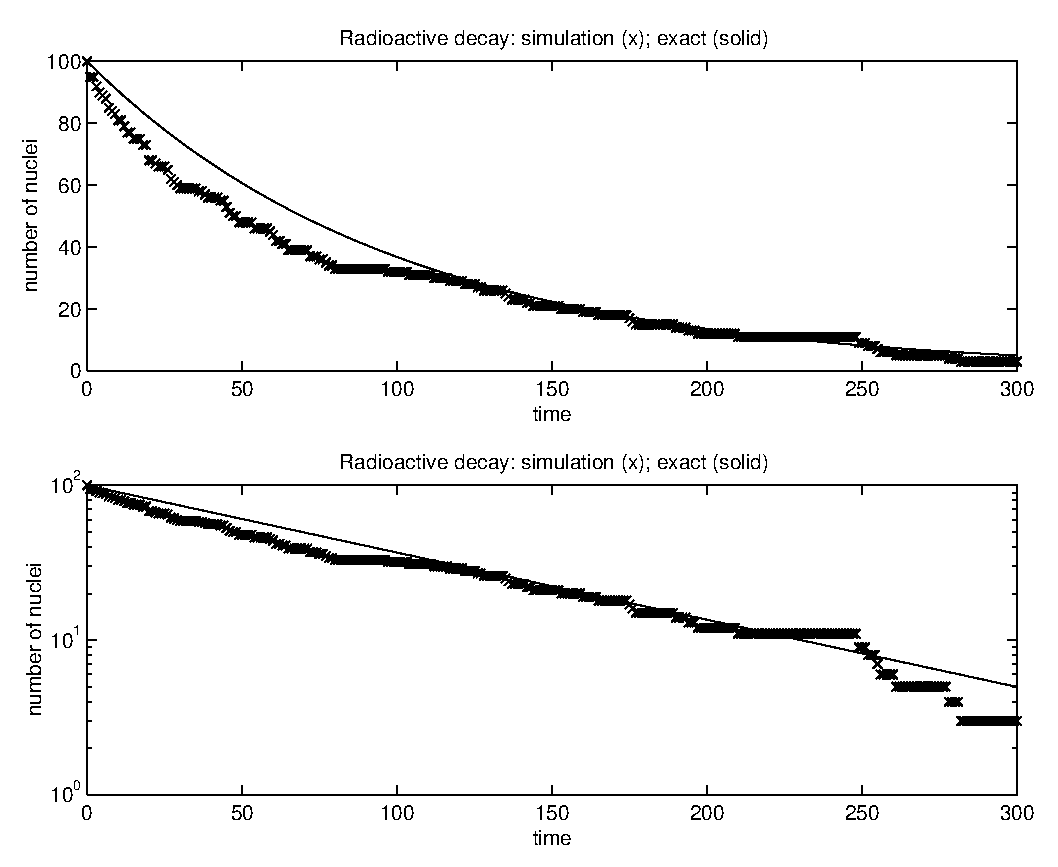
\includegraphics[width=10cm]{f_decaya.eps}
\caption{A realization of the stochastic process of radioactive decay.
The parameters of the simulation were $N_0 = 100; 
\quad p = 0.01 s^{-1}; \quad \Delta t = 1s;  \quad tend = 300s$}
\end{figure}
\begin{figure}
\label{FIG_DECAYB}
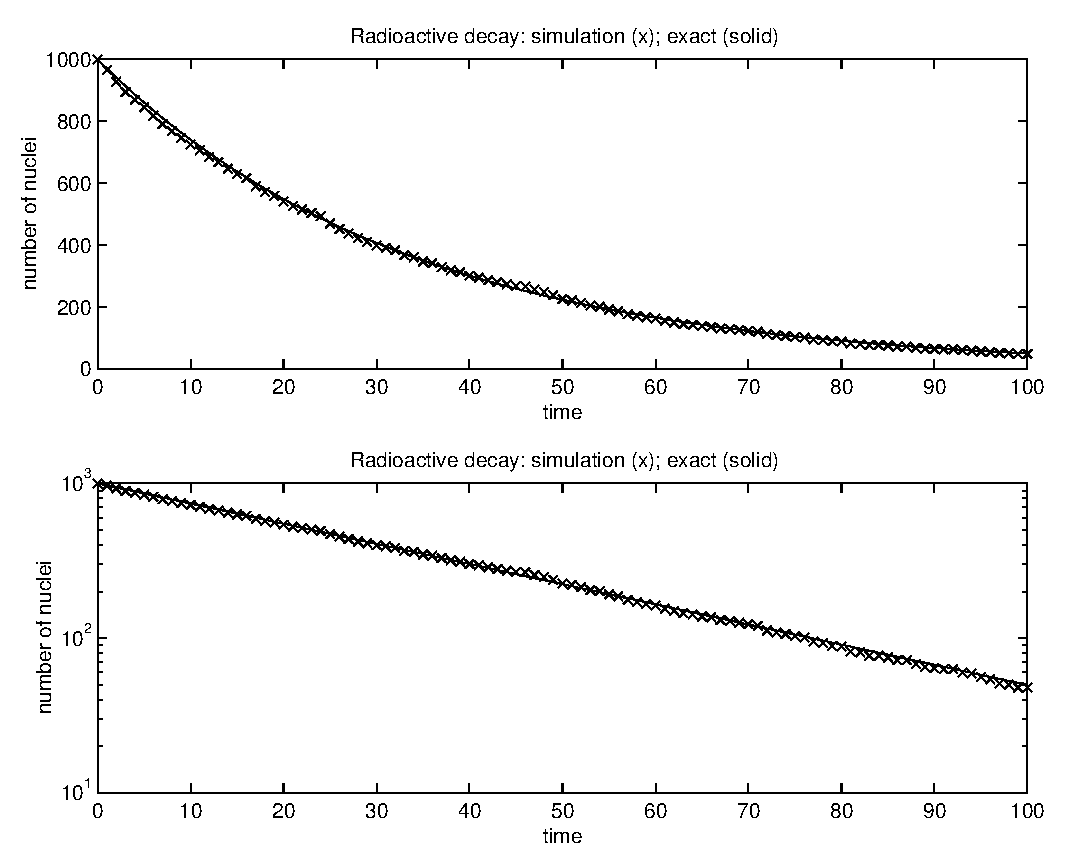
\includegraphics[width=10cm]{f_decayb.eps}
\caption{A realization of the stochastic process of radioactive decay.
The parameters of the simulation were $N_0 = 1000; 
\quad p = 0.03 s^{-1}; \quad \Delta t = 1s;  \quad tend = 100s$}
\end{figure}
 It is 
immediately recognized that the simulation results fluctuate around 
the expected curve. This is of course not astonishing since the 
exact result holds for mean values. In order to achieve a better
agreement with the decay law it is necessary to run the simulation
several times and to take the average over the different 
realizations of the decay process. This can easily be achieved by 
a simple modification of the program {\sf decay}. We 
introduce an additional input variable, the number of realizations
{\sf nreal} and accordingly implement a loop over the different 
realizations. This can be best seen in the listing of the 
new program {\sf decayr}.


At the end of the realizations loop
we have to perform the average. This is seen in lines xy.
(STRESS MORE THE IDEA OF REALIZATIONS!!!!; allgemeine Strategie erlaeutern.)

Note that in order to speed up the program we have modified slightly 
the algorithm  so that we can save a loop.
The probability to observe one decay in time $\Delta t$ is
\begin{equation}
p = \beta \Delta t
\end{equation}
where $\beta = \lambda N$ and $\Delta t$ must be small enough so 
that $\beta \delta t \ll 1$. 
From the elementary rules of combinatorics we know that
the probability to observe $n$ decays in time $t=m\Delta t$ is therefore
given by
\begin{equation}
P = p^n(1-p)^{m-n} {m \choose n}.
\end{equation}
Inserting the definition of $p$ the above expression can be cast 
in the form
\begin{equation}
P = \left( \frac{\beta t}{m}\right)^n 
     \left( \frac{1 - \beta t}{m} \right)^{m-n}
      \frac{m!}{(m-n)! n!}.
\end{equation}
Performing the limit $\Delta t \longrightarrow 0$ (i.e. $m 
\longrightarrow \infty$) and considering that
\begin{equation}
\left(1-  \frac{\beta t}{m} \right)^{m} \longrightarrow 
            \exp(-\beta t),
\end{equation}
\begin{equation}
\left( 1- \frac{ \beta t}{m} \right)^{-n} \longrightarrow 
            1,
\end{equation}
and
\begin{equation}
\frac{m!}{(m-n)! n!} \longrightarrow m^n
\end{equation}
we obtain the result
\begin{equation}
P = \frac{\mu^n \exp(-\mu)}{n!},
\end{equation}
where $\mu = \beta t$. The above distribution is the well know
Poisson distribution.

It is now easy to verify that the number of decays in a given 
interval is distributed according to the Poisson distribution.
To this end we have counted the number of decays in a given 
interval. This is accomplished in the lines xy. At the end of the
program we plot in a histogram the distribution of the number of 
decays and overlay the expected Poisson
distribution.  This is achieved in the program {\sf decayr} with the 
help of the {\sf hold} command. When you set "{\sf hold on}" MATLAB does not 
remove the existing graph; the following data are addeded to the 
current graph. The overplotting of data is terminated by 
setting "{\sf hold off}".

\subsubsection{Listing of the program decayr}
\inputlisting{./Listings/decayr.m}


Run the program for the following two sets of parameters:
\begin{eqnarray*}
N_0= 100, p = 0.001 s^{-1}, \Delta t = 1s, t = 100s \\
N_0= 100, p = 0.0001 s^{-1}, \Delta t = 1s, t = 100s
\end{eqnarray*}
with nreal = 100 and nreal = 1000.

The result of  two simulations can be seen in figs. x and y.
\begin{figure}
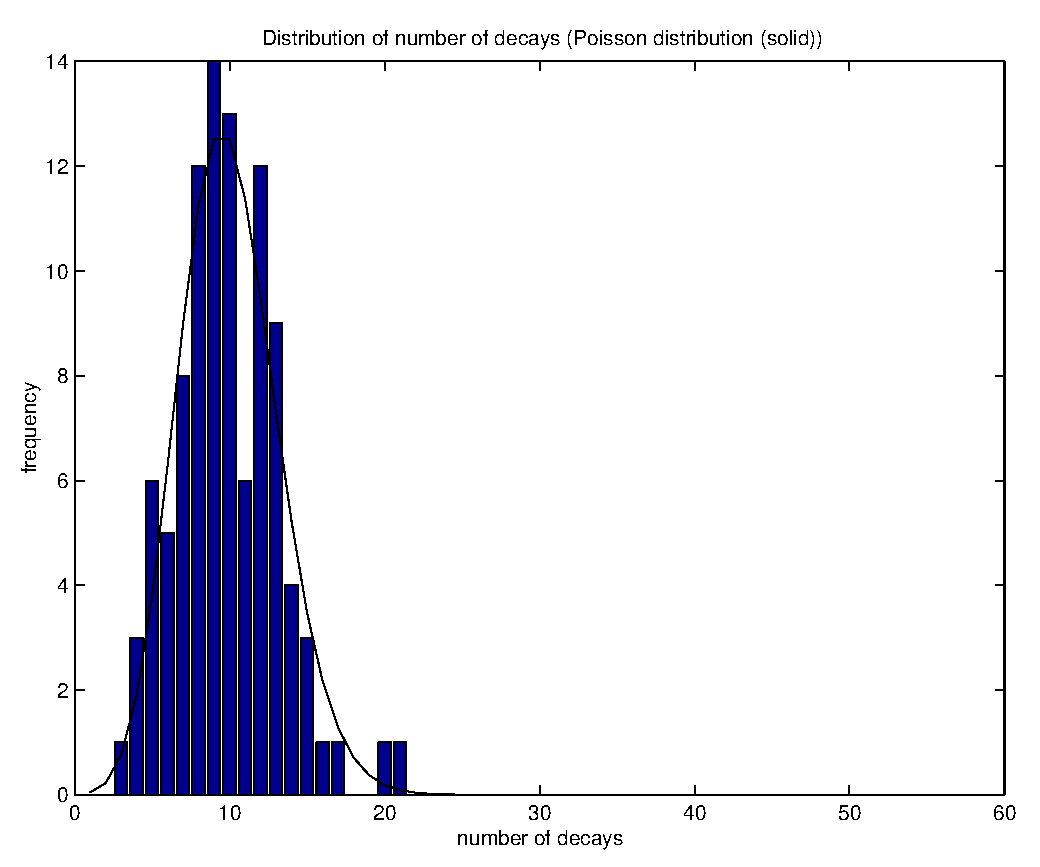
\includegraphics[width=\textwidth]{f_decay1.eps}
\caption{The distribution of the number of decays computed with 
the program decayr. 100 realizations. The simulation was run for
N0=100 and lambda=0.001.}
\end{figure}

\begin{figure}
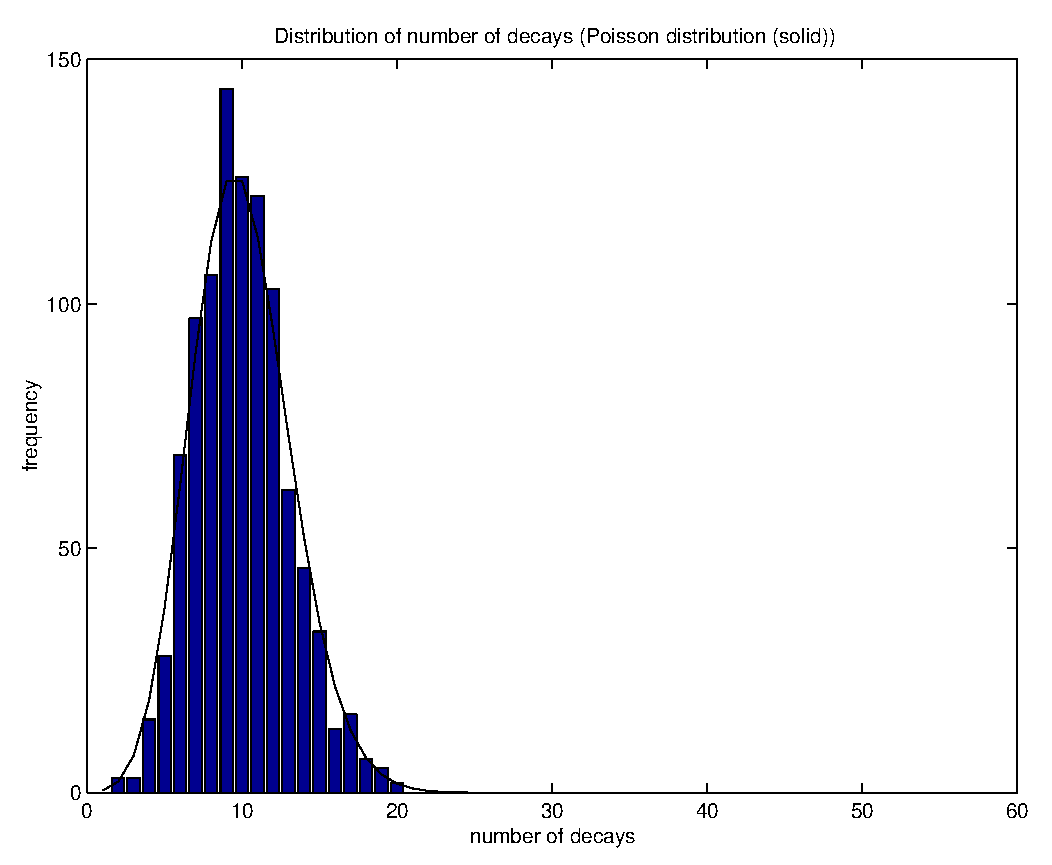
\includegraphics[width=\textwidth]{f_decay2.eps}
\caption{The distribution of the number of decays computed with 
the program decayr. 1000 realizations. The simulation was run
for N0=100 and lambda = 0.001.}
\end{figure}

%%%%%%%%%%%%%%%%%%%%%%%%%%%%%%%%%%%%%%%%%%%%%%%%%%%%%%%%%%%%%%%%%%%%%%
\section{Simple Monte Carlo evaluation of integrals}
It is the purpose of this subsection to introduce Monte Carlo Methods
in the context of the numerical evaluation of definite integrals.
We will see in later chapters that Monte Carlo integration is the
method of choice when treating multidimensional
integrals numerically. As a typical rule of thumb
``classical'' deterministic methods are outperformed
by Monte Carlo methods  for systems with a large number of 
degrees of freedom.
For simplicity and to stress the basic ideas 
it is convenient at the moment to consider one--dimensional definite
integrals of the form
\begin{equation}
\label{INTEGRAL}
I = \int_a^b dx f(x).
\end{equation}
Obviously such integrals can be evaluated analytically for many
integrands
$f(x)$.  However, there are as well many cases for which a numerical
evaluation is necessary.

Before introducing the Monte Carlo approach to numerical integration
let us remind the basic ``classical'' deterministic approach to
numerical integration. The standard approach is based upon the
geometrical interpretation of the integral (\ref{INTEGRAL}) as the
area under the curve of the function $f(x)$ between the points $a$ and
$b$. In the simplest algorithm this area (see figure) is approximated
as a sum over rectangles. To this end the $x$--axis is divided into
$n$ equally spaced intervals of width $\Delta x$,
\begin{equation}
\Delta x = \frac{b-a}{n}
\end{equation}
whose ends are given by
\begin{equation}
x_i = x_0 + i\Delta x
\end{equation}
for $i=1, \ldots ,n$. Of course, $x_0 = a$ and $x_n =b$. Thus in the
so--called rectangular approximation the integral is evaluated as
\begin{equation}
\label{I_CLASSICAL}
I_n = \Delta x \sum_{i=0}^{n-1} f(x_i).
\end{equation}
Of course, other more accurate approximations are possible.

How can we now evaluate the above integral by drawing random numbers?
The standard way is based on a very simple idea. 
From the introductory course in analysis we know that the Mean 
Value Theorem states that the exact value of the integral $I$ is 
given by
\begin{equation}
I= (b-a) f(\zeta)
\end{equation}
for some value of $\zeta$ in the interval $a \le \zeta \le b$. $f(\zeta)$
represents the average value of the function $f(x)$ 
in the interval $[a,b]$. Thus we could also write
\begin{equation}
I = (b-a) \langle f \rangle,
\end{equation}
where $\langle  \rangle$ denotes the mean value.
Let us draw $n$
random numbers which are uniformly distributed in the interval $[a,b]$
and let us sample the corresponding value of $f(x_i)=f_i$. The Monte Carlo
estimate $I_n$ of the integral $I$ is then the sample mean, which is
given by
\begin{equation}
\label{MCI_STANDARD}
I_n = \frac{(b-a)}{n} \sum_{i=1}^{n} f(x_i),
\end{equation}
where $n$ is the number of trials. Amazingly the form of the above
estimate is very similar to the classical formula (\ref{I_CLASSICAL}).
The fundamental difference is that now the $n$ points at which the
function $f$ is evaluated are no longer equally spaced but randomly 
distributed.

There is also the possibility to compute the integral $I$
stochastically
with the help of the ``Hit or Miss'' algorithm. The idea behind
this algorithm is again very simple. To be explicit we imagine a rectangle
of height $h$ and width $(b-a)$ such that the function $f(x)$ lies
within the rectangle (see figure; Gould, p.329). To evaluate the
integral we draw randomly pairs of uniformly distributed random
numbers $(x_i,y_i)$ such that $a \le x_i \le b$ and $0 \le y_i \le h$.
In other words the probability to draw a point within the rectangle is
given by the inverse of the area $A$ of the rectangle,
i.e. $1/(b-a)h$. It is now evident how the area under the
function $f$ may be estimated. The fraction of points $(x_i,y_i)$
which satisfy the condition $y_i \le f(x_i)$ is an estimate of the
ratio of the integral $I$ to the area $A$ of the rectangle. Hence,
drawing $n$ random pairs the estimate $I_n$ of $I$ by this ``scoring''
method is given by
\begin{equation}
I_n = A \frac{n_s}{n},
\end{equation}
where $n_s$ is the number of ``hits'', i.e., of points lying below the
curve $f(x)$.

Before writing two simple programs to elucidate the above algorithms
it is important to have in mind that both estimates are affected by
statistical errors. Let us consider for simplicity 
the standard method. Since the $f(x_i)$ are random we know 
from the elementary theory of data analysis
that an appropriate measure of the error is given by the variance
which is defined by
\begin{equation}
{\rm Var}(f) = \langle f^2 \rangle - \langle f \rangle^2.
= \langle (f -\langle f \rangle)^2 \rangle
\end{equation}
Since we draw a finite number of random numbers we can
estimate the mean value by using
\begin{equation}
\hat{f}  = \frac{1}{n} \sum_{i=1}^n f(x_i) 
\end{equation}
and correspondingly the estimate of the variance by using
\begin{equation}
{\rm Var}(f(x_1),\ldots, f(x_n)) = \frac{1}{n-1} \sum_{i=1}^n 
   (f(x_i)- \hat{f})^2 = \sigma_f^2.
\end{equation}
The quantity $\sigma_f = \sqrt{{\rm Var}(f_1, \ldots, f_n)}$ 
is also called the standard deviation. In the previous expression
we have used the short--hand
notation $f(x_i) = f_i$. However,
we are not interested in the error of $f$ but in the error of the
estimate $I_n$ which is a sum over random numbers. 

Repeating the 
simulation and hence drawing other random numbers we will get another
estimate of $I_n$. Therefore, repeating the simulation $m$ times 
we can estimate the mean of $I_n$ as
\begin{equation}
\hat{I_n} = \frac{1}{m} \sum_j^m I_n(j)
\end{equation}
and the corresponding variance as
\begin{equation}
{\rm Var}(I_n(1), \ldots, I_n(m)) = 
\frac{1}{m-1} \sum_j^m (I_n(j) - \hat{I_n})^2 = \sigma_I^2
\end{equation}
We will denote the above variance also by $\sigma_I^2$.
Of course, proceeding this way is not very practical since we
have to perform the simulation $m$ times. A much more economical
estimation of the error of the mean of $I_n$ could be achieved by 
establishing a simple relation between $\sigma_I$ and the standard 
deviation of the individual trials $\sigma_f$. To this end we 
introduce the discrepancy $\delta f_i$ between the
individual trial $f_i$ and its mean $\langle f \rangle$. The 
discrepancy $\delta I_n$ between $I_n$ and its mean value can be
obtained to first order in the $\delta f_i$ by a simple Taylor 
expansion (error propagation rules)
\begin{equation}
\delta I_n = \sum_{i=1}^n \frac{\partial I_n}{\partial f_i} \delta 
f_i.
\end{equation}
Hence, it follows from the above equation by taking the average over
$\delta I_n^2$ that
\begin{equation}
\langle \delta I_n^2 \rangle = \sum_{i,j=1}^{n}
    \frac{\partial^2 I_n}{\partial f_i \partial f_j} 
     \langle \delta f_i \delta f_j \rangle.
\end{equation}
It is plausible to assume, that 
$\langle \delta f_i \rangle = 0$
for all $i$ and that the $\delta f_i$ are not correlated
for $i \neq j$, i.e.,
$\langle \delta f_i \delta f_j \rangle = \langle f_i \rangle \langle f_j \rangle$
and that for $i=j$ we have $\langle \delta f_i^2 \rangle = \sigma_f$ 
for all $i$ it follows from the above equation that
\begin{equation}
\sigma_I^2 = \sum_{i=1}^n \left(
      \frac{\partial I_n}{\partial f_i} \right)^2 \sigma_f^2
      = \frac{1}{n^2} n \sigma_f^2 = \frac{\sigma_f^2}{n}
\end{equation}
and finally we have the useful relation
\begin{equation}
\sigma_I = \frac{\sigma_f}{\sqrt{n}}.
\end{equation}
The mean error of the mean scale with 1 over the square root of 
the number of individual trials. The precision of the estimate 
thus increases only slowly with the number of trials (remark: central
limit theorem: see Chapter 2).

Now we are in the position to write two programs to implement the above
stochastic algorithms. In order to be specific we compute the integral
\begin{equation}
I = \int_0^1 dx \sqrt{1-x^2} = \frac{\pi}{4}.
\end{equation}
In other words we want to estimate the number $\pi$ by Monte Carlo
methods.

We begin by the standard method. The listing of an according 
program can be seen below.

\subsubsection{Listing of the program mcpi.}
\inputlisting{./Listings/mcpi.m}

We run the program for $n=10, 100, 1000, 10000$. The result of the 
four simulations can be seen in Fig. xy.
\begin{figure}
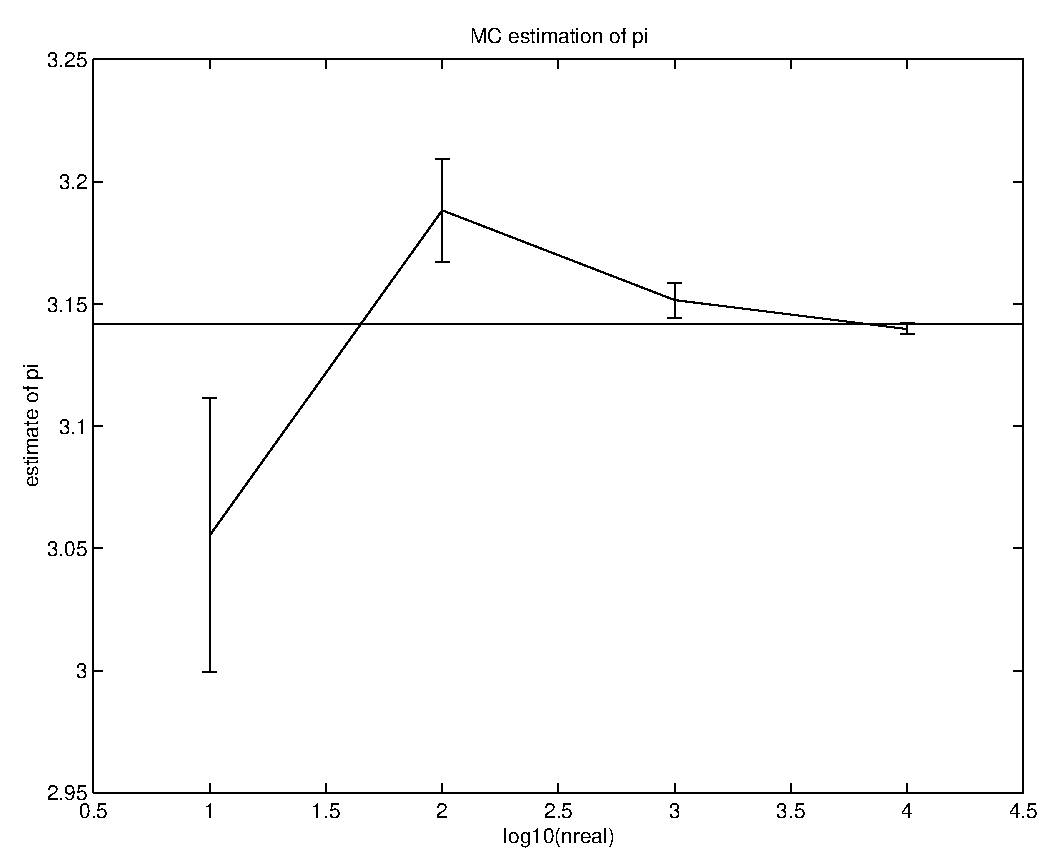
\includegraphics[width=\textwidth]{plotmcpi.eps}
\caption{The estimation of pi for n=10,100,1000,10000. The 
error bars correspond to the standard deviation of the mean of the 
estimate.}
\end{figure}

Next we write a program for the scoring  method. 

\subsubsection{Listing of the program mcpiscore.m}
\inputlisting{./Listings/mcpiscore.m}

Again we run the simulation for n=10, 100, 1000, 10000.
The result of a simulation can be seen in the next Figure.
\begin{figure}
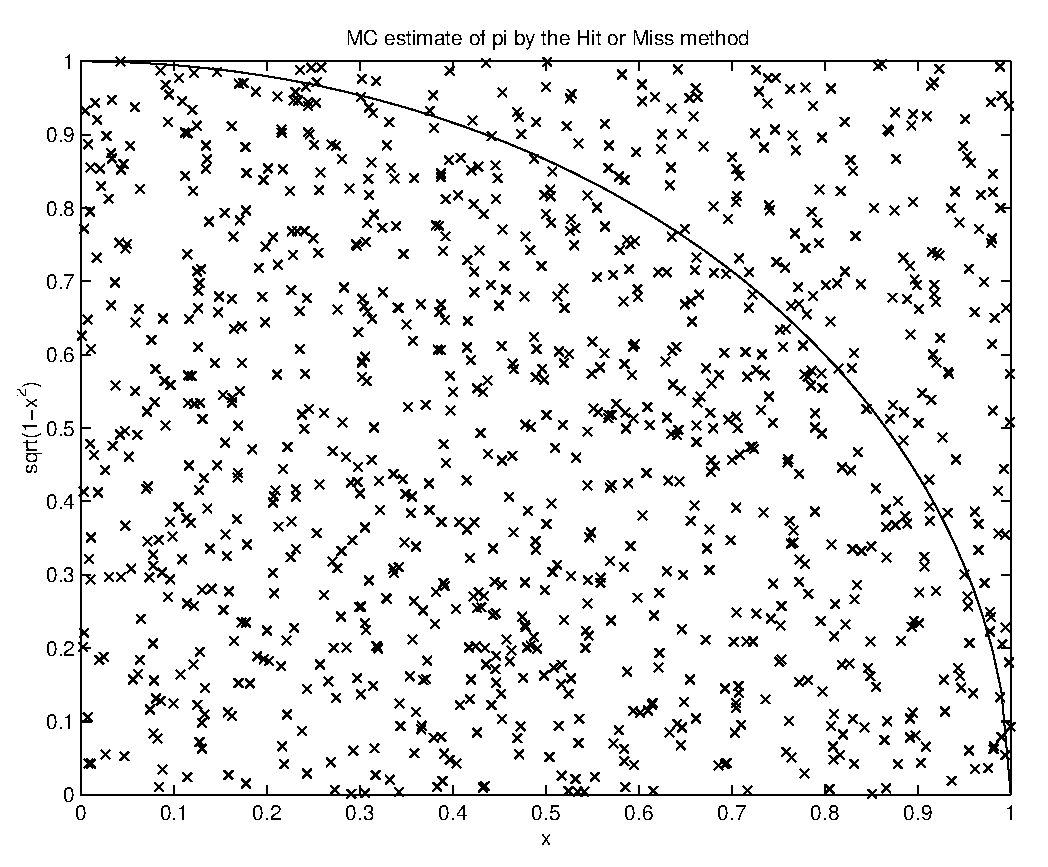
\includegraphics[width=\textwidth]{fmcpiscore.eps}
\caption{The scoring method. The continuous line represents
the function $\sqrt{(1-x^2)}$.}
\end{figure}


%%%%%%%%%%%%%%%%%%%%%%%%%%%%%%%%%%%%%%%%%%%%%%%%%%%%%%%%%%%%%%%%
\section{Beyond this chapter}


%%%%%%%%%%%%%%%%%%%%%%%%%%%%%%%%%%%%%%%%%%%%%%%%%%%%%%%%%%%%%%%%
\section{Exercises}
{\bf Exercise 1.} Write a program to simulate photoabsorption.
    Lit. Whitney

{\bf Exercise 2.} Write a program for the Monte Carlo estimation of
the following integral
\begin{equation}
\int_0^1\frac{dx}{1+x^2} = \frac{\pi}{4}
\end{equation}

{\bf Exercise 3.} Write a program to evaluate the number $e$ by a
stochastic method.
Lit: Pirooz Mohazzabi, Monte Carlo estimation of $e$,
Am. J. Phys. {\bf 66} (1998) 138--140.


\bibliographystyle{peter}
\bibliography{V_98}


%%% Chapter 2 
%%%%%%
%%%%%% Chapter 2
%%%%%%

\chapter{Stochastic Variables}
Since the notion of random variables will be essential
for the understanding of stochastic methods this chapter will be 
devoted to the introduction of the fundamental concepts of 
probability theory.

%%%%%%%%%%%%%%%%%%%%%%%%%%%%%%%%%%%%%%%%%%%%%%%%%%%%%%%%%%%%%%%%%%
\section{The nature of probabilities}
In the previous chapter we have already made use of probabilistic 
notions in an intuitive way. However, we have not asked the 
following question: What are probabilities? How can we formulate 
the notion of probability in such a way that it is useful for 
physical applications?

Essentially, there are three possible definitions of probability
\cite{BRODY}:
a) the axiomatic interpretation, b) the frequency interpretation, and
c) the ensemble interpretation.


\subsection{The axiomatic interpretation}
The axiomatic definition \cite{FELLER} of probabilities has been proposed by 
Kolmogorov in 1933. The formal objects to which we want to 
attribute probabilities are called {\em events} and are subsets
of a basic set $\Omega$ which is called the {\em event space} or in 
physical applications the {\em phase space}. If the event $e$ 
belongs to $\Omega$, so does its complement $\Omega - e$ also; the 
null event $\oslash$ is therefore also in $\Omega$. Events 
containing only one member of $\Omega$ are called the elementary events
of $\Omega$.

A function $P(e)$, called the {\em probability} of $e$ can be 
assigned to each event $e$ in $\Omega$. The function $P(e)$ has
the following properties:

(i) $P(e) \ge 0$ for all $e$ in $\Omega$;

(ii) $P(\Omega) = 1$;

(iii) If $e_1, e_2, \ldots $ are in $\Omega$ and are pairwise
disjoint, i.e., $e_i \cap e_j = \oslash$ when $i \ne j$, then
$P(e_1 \cup e_2 \cup \ldots ) = P(e_1)+P(e_2) + \ldots$.

It follows immediately from the above three axioms that

(iv) If $\bar{e}$ is the complement of $e$, i.e., the set of all 
events which are not in $e$, then
$P(\bar{e}) = 1- P(e)$;

(v) $P(\oslash) = 0$.



\subsection{The relative frequency interpretation}
In his attempt to axiomatize probability theory, von Mises
introduced in 1919 the notion of a {\em Kollektiv}, which stands
for a single infinite sequence of random events such as the 
outcomes of throwing a coin. He defined then the probability of some 
event to be the limit of its relative frequency in such a series of 
observations when the series becomes infinitely long (the 
Kollektiv) \cite{COMPAGNER,BRODY}. 
If we denote by $n$ the number of data in the series,
by $m(e)$ the number of times the event is observed in it, then
the probability $P(e)$ is defined as
\begin{equation}
P(e) = \lim_{n \rightarrow \infty} \frac{m(e)}{n}.
\end{equation}
Of course, such a series of events must have the property that any 
infinite subsequence in it must have the same limit. 

The problem with this definition is the following one: How can any 
sequence of experimental data, which will be always be finite, 
have the properties of such a Kollektiv? In practice the 
relative frequencies for subsequencies will always differ from 
that in the main sequence.

To illustrate the problems with the frequency interpretation of
probabilities we consider the following example. We throw a die 
$n$ times and
look at the relative frequency $m(4)$ of the outcome of throwing a 
4. This experiment will be simulated with the help of the 
following program.

{\bf Listing of the program relfreq.}
\inputlisting{./Listings/relfreq.m}

The result of an experiment for up to 400 throws is shown in Fig. 
(\ref{F_FRELFREQ}). Running the program again we observe 
another approach to the asymptotic
value. We recognize immediately the difficulties with von Mises 
definition of probability.
\begin{figure}
\label{F_FRELFREQ}
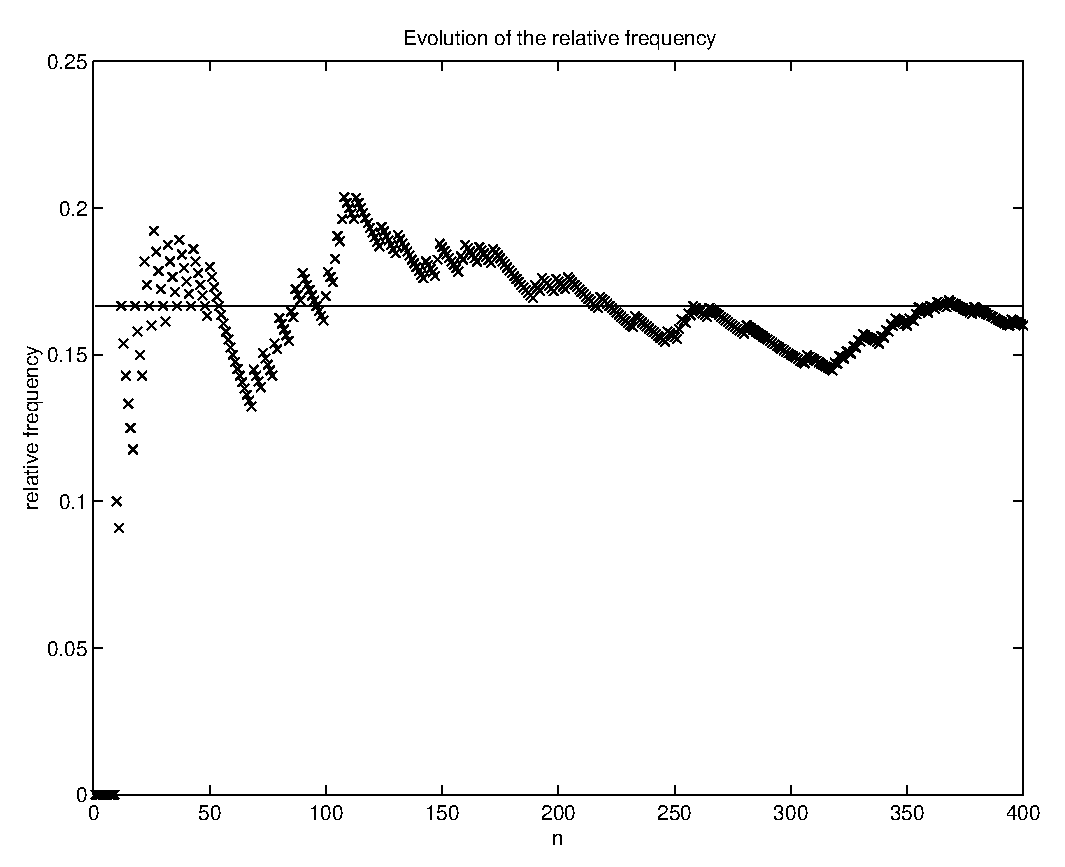
\includegraphics[width=10cm]{frelfreq.eps}
\caption{Simulation of the evolution of the relative frequency of throwing
a 4 in play of die.}
\end{figure}

\subsection{The ensemble interpretation}
We know from statistical mechanics  the notion of {\em ensemble}. An
ensemble is a collection of a large number $N$ of equally prepared
systems (equal models). A simple example is the microcanonical
ensemble, 
which is the
ensemble of all microstates in phase space, which are characterized by
fixing the macroscopic values for the the energy $E$, the volume $V$
and the number of particles $N$.

The abstract concept of an ensemble allows naturally the definition
of a mean value. We have to consider two cases:

(i) The ensemble contains a finite, discrete number of models: 
Let $n$ be the number of models and $Q(i)$ the interesting quantity in
model $i$. The ensemble mean value $\langle Q \rangle$ is then defined
as
\begin{equation}
\langle Q \rangle = \sum_{i=1}^n \frac{Q(i)}{n}.
\end{equation}

(ii) The models are characterized by some continuous parameter, i.e.,
the initial positions of molecules in a gas: If we name the continuous
parameter $\omega$, the phase space as $\Omega$ , and $n(w)$ a weight
function characterizing the ensemble, then
\begin{equation}
\langle Q \rangle = \frac{ \int_{\Omega} Q(\omega) dn(\omega)}
                         {\int_{\Omega} dn(\omega)}.
\end{equation}
Usually, the function $n(\omega)$ can be derived on the basis of the
theoretical model on which the ensemble relies upon. 

Let us consider as a simple example from equilibrium statistical 
mechanics a gas consisting of $N$ particles. The microstates of 
the system are the points $(q,p) = (\vec{r}_1, \vec{r}_2, \ldots, \vec{r}_N,
\vec{p}_1,\ldots, \vec{p}_N)$ in the 6--dimensional phase space.
The probability to find the microsystem at time $t_0$ in a volume 
element $dV=d^{3N}qd^{3N}p$ around $(q,p)$ is given by
\begin{equation}
dw(q,p) = \rho(q,p) d^{3N}qd^{3N}p,
\end{equation}
where $\rho(q,p)$ is the distribution function. For the 
microcanonical ensemble  the distribution function $\rho$ simply 
reads
\begin{equation}
\rho(q,p) = \left\{ 
\begin{array}{ll}
c= {\rm const}, &{\rm for} \quad E-\Delta \le H(q,p) \le E, \\
0, &{\rm otherwise}
\end{array} \right.
\end{equation}

Probabilities can be introduced as a special kind of ensemble 
average. Let $A$ be a property, which 
the members of the ensemble may have or not and let us define an indicator
function
\begin{equation}
\chi_A(\omega) = \left\{ 
\begin{array}{ll}
1, & {\rm if \quad member \quad labelled} \quad \omega {\rm \quad has 
\quad property\quad} A \\
0, & {rm if not}.
\end{array}\right.
\end{equation}
The probability of $A$ in the ensemble is  simply defined as 
the ensemble average of $\chi_A(\omega)$
\begin{equation}
P(A) = \langle \chi_A(\omega) \rangle = 
\frac{\int_{\Omega} \chi_A(\omega) dn(\omega)}{\int_{\Omega} 
dn(\omega)}.
\end{equation}
The probability is the relative weight in the ensemble of those 
members that have the property $A$. In the case of a discrete 
ensemble the above definition of probability reduces to a sum over
the members of the ensemble having the property $A$
\begin{equation}
P(A) = \sum_{i=1}^{n} \frac{\chi(i)}{n},
\end{equation}
i.e., the probability is the relative frequency of the members 
having the property $A$ in the ensemble.

It is clear that from the above definition of probability its is
possible to derive the Kolmogorov axioms of probability theory.

It is important to stress that the
ensemble is a purely theoretical construction and has to be adapted 
to the physical situation of interest as we will see in the future chapters. 
Furthermore, it is to be noted that the ensemble 
interpretation  allows the definition of time dependent 
probabilities,
i.e.,
\begin{equation}
P(A,t) = \langle \chi_A(t) \rangle,
\end{equation}
which are of fundamental importance while studying stochastic 
processes.

%%%%%%%%%%%%%%%%%%%%%%%%%%%%%%%%%%%%%%%%%%%%%%%%%%%%%%%%%%%%%%%%%%
\section{The definition of stochastic variables}
A stochastic variable $X$ is an object which is defined by a space 
of states (space of events, phase space) and by a probability 
density over this set. The space of state may be discrete, e.g. 
the numbers 1,2,3,4,5,6 for a play of dice or the number of 
molecules in a chemical reaction, as well as continuous, e.g.
the velocity of a Brownian particle. Of course, the space of state
may also be discrete and continuous at the same time, e.g., the
energy of an electron in the presence of some binding centers.
When sampling a one dimensional continuous stochastic variable $X$,
the probability to find some value in the infinitesimal interval
$(x,x+dx)$ will be expressed symbolically by
\begin{equation}\label{DENSITYDEF}
P(x) dx \equiv {\rm Prob} \{X\in [x,x+dx] \},
\end{equation}
which defines the probability density $P(x)$ associated with the 
stochastic variable $X$. It follows immediately from the above 
equation and from the addition law of
probability theory that the probability to sample a value of $X$
in the interval $[a,b]$ is given by
\begin{equation}\label{DENSITYDEF2}
\int_a^b dx P(x) = {\rm Prob}\{ X \in[a,b] \}.
\end{equation}
It is evident from Eqs. (\ref{DENSITYDEF}) and (\ref{DENSITYDEF2}) that 
the probaility density is non--negative, i.e. $P(x) \ge 0$ and 
that it is normalized
\begin{equation}
\int_{-\infty}^{\infty} dx P(x) = 1.
\end{equation}
For later convenience we remark that the probability density may 
contain also sums over $\delta$--functions. For example $P(x)$ can 
also have the form 
\begin{equation}
P(x) = \sum_n p_n \delta(x-x_n) + \tilde{P}(x),
\end{equation}
where
$\tilde{P}(x) \ge 0$, $p_n \ge 0$, $\tilde{P}$ integrable  
and the normalization condition is
\begin{equation}
\sum_n p_n + \int dx \tilde{P}(x) =1.
\end{equation}

The distribution function $F$ of the stochastic variable $X$ is 
defined by 
\begin{equation}
F(x) \equiv {\rm Prob}\{X \le x\}.
\end{equation}
The density function and the distribution function are related by 
the equation
\begin{equation}
F(x) = \int_{-\infty}^x dx' P(x'),
\end{equation}
or equivalently by $F'(x)= P(x)$.

\subsection{Further characterization of stochastic variables}
A stochastic variable is completely defined by the space of states 
and by the probability density function. However, it is helpful to 
introduce some other quantities in order to characterize them.

The {\em expectation value}, i.e. the average,  of any function $f(X)$ 
with respect to the stochastic variable $X$ is denoted by
$\langle f(X) \rangle$ and is defined by
\begin{equation}
\langle f(X) \rangle = \int dx f(x) P(x).
\end{equation}
Of particular importance are the {\em moments} of a distribution. The 
$m$--th moment $\mu_m$ is defined as $\langle X^m \rangle$. Of 
course, $\mu_1$ is the {\em mean}. The variance ${\rm Var}(X)$ 
is defined as
\begin{equation}
{\rm Var}(X) \equiv \langle (X - \langle X \rangle )^2\rangle
   = \mu_2 - \mu_1^2,
\end{equation}
and is the square of the standard deviation $\sigma$.

Another important quantity is the {\em characteristic function} $G(k)$. It is 
defined as
\begin{equation}
G(k) = \langle \exp(ikx) \rangle = \int_I \exp(ikx) P(x) dx,
\end{equation}
and has the obvious properties
\begin{equation}
G(0) = 1 \quad {\rm and} \quad |G(k)| \le 1.
\end{equation}
The characteristic function is also called the {\em the moment 
generating function}, because expanding the exponential function 
in a Taylor series we get 
\begin{equation}
G(k) = \sum_{n=0}^{\infty} \frac{i^n}{n!} k^n 
      \langle X^n \rangle.
\end{equation}
Thus, if $G(k)$ is known the moments are easily evaluated as
\begin{equation}
\left. \frac{d^n}{dk^n}G(k) \right| = i^n \langle X^n \rangle.
\end{equation}
The same function serves to generate the so--called cumulants
which are defined as
\begin{equation}
\ln G(k) = \sum_{n=1}^{\infty} \frac{(ik)^n}{n!} \kappa_n,
\end{equation}
and are combinations of the moments, i.e., the first three 
cumulants are given by
\begin{eqnarray}
\kappa_1 &=& \mu_1, \\
\kappa_2 &=& \mu_2 - \mu_1^2 =\sigma^2, \\
\kappa_3 & = & \mu_3 - 3 \mu_2 \mu_1 + 2 \mu_1^3.
\end{eqnarray}
It can be shown \cite{Gardiner} that the cumulant generating 
function  cannot be a polynomial of degree greater than 2, that 
is, either all but the first two cumulants vanish or there is an 
infinite number of nonvanishing cumulants.

REMARK ( kappai given then g(k) unique !!!???????????�) 

\subsection{Some important random variables}
Let us first introduce and discuss briefly some important 
continuous one dimensional probability densities.

\subsubsection{The uniform density}
The simplest density is the uniform density which is constant if $x$
lies within the interval $[a,b]$ and zero otherwise, i.e.,
\begin{equation}
P(x) = 1/(b-a).
\end{equation}
It is easy to check that the mean of the uniform distribution is
\begin{equation}
\langle X \rangle = \frac{a+b}{2}
\end{equation}
and that the standard deviation of a uniformly distributed random variable 
is
\begin{equation}
\sigma = \frac{b-a}{2\sqrt{3}}.
\end{equation}
As we will see the uniform probability density will play a 
fundamental role in the forthcoming chapters.

\subsubsection{The exponential density function} 
The exponential density function is defined as
\begin{equation}
P(x) = a \exp(-ax),
\end{equation}
where $a$ is any positive constant. It is easy to verify that
the mean and the standard deviation of an exponentially distributed random 
variable are equal
\begin{equation}
\langle X \rangle = \sigma = \frac{1}{a}.
\end{equation}

\subsubsection{The Gaussian or normal density function}
The most important density function for physics is the 
gaussian probability density. It has the form
\begin{equation}
P(x) = (2\pi a^2)^{-1/2} \exp[-(x-x_0)^2/2a^2],
\end{equation}
for $a$ positive and $-\infty < x_0 < \infty$.
The mean and the standard deviation of the Gaussian probability 
density are given by $\mu_1 = x_0$ and by $\sigma =a$, 
respectively. The characteristic function of the Gaussian density reads
\begin{equation}
G(k) = \exp(i \mu_1k - \frac{1}{2} \sigma^2 k^2),
\end{equation} 
which means that $\kappa_1 = \mu_1$, $\kappa_2 = \sigma^2$ and 
that all higher cumulants vanish.

\subsubsection{The Cauchy or Lorentz density} 
The Cauchy or Lorentz density is defined as
\begin{equation}
P(x) = \frac{1}{\pi} \frac{a}{(x-x_0)^2 + a^2}
\end{equation}
for positive $a$ and $-\infty <x_0 < \infty$. It is an example of 
a probability density which does not have a finite variance. In 
fact, not even the integral defining  the mean value converges. 

Let us now discuss some typical discrete probability densities.
The discrete random variable will be denoted by $N$.

\subsubsection{The discrete uniform probability density} 
The discrete uniform probability density is defined by
\begin{equation}
P(n) = \frac{1}{n_2 -n_1 +1}
\end{equation}
for $n_1 \le n \le n_2$ and zero otherwise. Of course,
$n_1$ and $n_2$ are integer numbers and $n_1 \le n_2$.
Its mean value is
\begin{equation}
\langle N \rangle = \sum_n n P(n) = \frac{n_1 +n_2}{2} 
\end{equation}
and its variance
\begin{equation}
\sigma^2 = \frac{(n_2 -n_1)(n_2 -n_1+2)}{12}.
\end{equation}
The above equations are easily proven with the help of the 
relations
\begin{equation}
\sum_{n=1}^N n= \frac{N(N+1)}{2}; \sum_{n=1}^{N} n^2 = \frac{N(N+1)(2N+1)}{6}. 
\end{equation}

\subsubsection{The binomial distribution}
Let us assume that the random variable $Y$ 
can take only two values $\{y_1,y_2\}$, the probability for the 
value $y_1$ being $p$ and correspondingly for $y_2$ (1-p). If we 
consider $N$ realizations of the stochastic variable $Y$ the 
probability to find the value $y_1$ $N$ times under the $n$ results
is the binomial density $P(n)$
\begin{equation}
P(n) = \frac{N!}{n!(N-n)!} p^n(1-p)^{(N-n)},
\end{equation}
for $0 \le n \le N$.
The mean and variance of the binomial density are given by
\begin{equation}
\langle n \rangle = Np,
\end{equation}
and
\begin{equation}
\sigma^2 = Np(1-p).
\end{equation}
It is easy to check the normalization of the binomial distribution since
\begin{equation}
1 = [p + (1-p)]^n = \sum_{n=0}^N \frac{N!}{n! (N-n)!}
        p^n (1-p)^{(N-n)}.
\end{equation}

\subsubsection{The Poisson density}
The Poisson density as we already know
is defined as
\begin{equation}
P(n) = \frac{\exp(-a) a^n}{n!},
\end{equation}
for $n > 0$ and $a \in R$. The mean value and the variance
of the Poisson density are equal,
\begin{equation}
\langle n \rangle = \sigma^2 = a.
\end{equation}
As we already know from the discussion of the radioactive decay the 
Poisson density is a limit of the 
binomial probability density for $N \rightarrow \infty$, $p \rightarrow 
0$ while $Np=a={\rm const}$. Another limit of the Poisson density
which deserves consideration is the limit $a \gg 1$: In this limit
the Poisson density will be essentially different from zero only 
for $n \approx a$. For $n \gg 1$  the Stirling formula 
holds
\begin{equation}
n! \approx (2 \pi n)^{1/2} n^n \exp(-n)
\end{equation}
so we can write
\begin{equation}
\ln\left[ \frac{\exp(-a) a^n}{n!} (2\pi a)^{1/2} \right] 
\approx (n-a) -n\ln\left(\frac{n}{a}\right).
\end{equation}
Setting $\epsilon=(n-a)/2$ and since, 
for $\epsilon \ll 1$ $\ln(1+\epsilon) \approx \epsilon -
\epsilon^2/2$ and for $n\approx a$
we can write
\begin{equation}
\ln\left[ \frac{\exp(-a) a^n}{n!} (2\pi a)^{1/2} \right] \approx
-(n-a)^2\frac{1}{2a}.
\end{equation}
So that finally for $a \gg 1$
\begin{equation}
\frac{\exp(-a) a^n}{n!} \approx \exp\left( - 
\frac{(n-a)^2}{2a}\right).
\end{equation}
Thus, in the limit $a \gg 1$ the Poisson density resembles a
Gaussian density with mean $a$ and variance $a$.

\subsection{Multivariate random variables}
Up to now we have considered only one dimensional stochastic 
variables. Obviously, $n$ random variables $X_1, X_2, \ldots, X_n$ 
which are sampled simultaneously can be interpreted as the 
components of an $n$--dimensional stochastic variable $X$.
Their joint density function
$P_n(x_1, \ldots, x_n)$ is defined through the statement
\begin{equation}
P_n(x_1, \ldots, x_n)dx_1 dx_2 \ldots dx_n \equiv
{\rm Prob}\{ X_i \in (x_i,x_i+dx_i) \quad \text{for 
each} \quad i=1, \ldots , n\}.
\end{equation}
If we look at the subset of stochastic variables $X_1, \ldots 
X_s$, for $s>n$ we can easily write down with the help of the
elementary laws of probability theory the joint density function for 
this set irrespective of $X_{s+1}, \ldots, X_n$
\begin{equation}
P_s(x_1, \ldots, x_s) = \int P_n(x_1, \ldots, x_s, x_{s+1}, \ldots 
x_n) dx_{s+1} \ldots dx_{n}.
\end{equation}
$P_s$ is a so--called {\em marginal distribution}.

The {\em conditional density} 
$P_{s|n-s}(x_1,\dots,x_s|x_{s+1},\ldots,x_n)$ is the joint 
density of $X_1, \ldots , X_s$
given that $X_{s+1}=x_{s+1}$, \ldots , $X_n = x_n$ and is easily 
shown to be given by Bayes rule
\begin{equation}
P_{s|n-s}(x_1,\dots,x_s|x_{s+1},\ldots,x_n) =
\frac{P_n(x_1, \ldots, x_n)}{P_{n-s}(x_{s+1}, \ldots, x_n)}.
\end{equation}

Two subsets $(X_1, \ldots, X_s)$ and $(X_{s+1}, \ldots, X_n)$ are 
said to be statistically  independent if $P_n$ factorizes
\begin{equation}
P_n(x_1, \ldots, x_n)=P_s(x_1, \ldots, x_s)P_{n-s}(x_{s+1}, \ldots, 
x_n).
\end{equation}
In this case $P_s$ is the marginal as well as the conditional 
probability density.

The definition of moments is easily generalized to the  
multivariate case
\begin{equation}
\langle X_1^{m_1} \ldots X_n^{m_n} \rangle =
\int x_1^{m_1} \ldots x_n^{m_n} P(x_1, \ldots, x_n) dx_1 \ldots 
dx_n.
\end{equation}
Accordingly, the characteristic function is given by
\begin{equation}
G(k_1, \dots, k_n) = \left\langle 
\exp[i(k_1X_1 + \ldots +k_n X_n)]\right\rangle.
\end{equation}
Again the multivariate Taylor expansion in the variables $k_i$ 
generates the moments
\begin{equation}
G(k_1, \dots, k_n) = \sum \frac{(ik_1)^{m_1} \ldots (ik_n)^{m_n}}
                  {m_1! \ldots m_n!} 
       \langle X_1^{m_1} \ldots X_n^{m_n} \rangle.
\end{equation}
For completness we mention that the cumulants 
$\kappa(X_1^{m_1} \ldots X_n^{m_n})$ are defined as
\begin{equation}
\log G(k_1, \dots, k_n) = {\sum}' \frac{(ik_1)^{m_1} \ldots (ik_n)^{m_n}}
                  {m_1! \ldots m_n!} 
       \kappa(X_1^{m_1} \ldots X_n^{m_n}),
\end{equation}
where the symbol $\sum'$ idicates that we do not have to sum when 
all $m$ vanish. As an example we give the $n \times n$ covariance
matrix $\kappa(X_i X_j)$
\begin{eqnarray}
{\rm Cov}(X_i, X_j) &=& 
 \langle (X_i-\langle X_i \rangle)(X_j-\langle X_j \rangle)\rangle 
 \\
 & = & \langle X_i X_j \rangle - \langle X_i \rangle \langle X_j 
           \rangle.
 \end{eqnarray}
The diagonal elements of the covariance matrix are, of course, the 
variances, whereas the off--diagonal elements are called the 
covariances.
With the help of the covariance matrix it is possible to define a 
correlation coefficient
\begin{equation}
\rho_{ij} = \frac{\kappa(X_i X_j)}{\sqrt{\kappa(X_i^2) 
\kappa(X_j^2)}}.
\end{equation}
For $n=2$ the statistical independence of $X_1$ and $X_2$ can be 
expressed through one of the following criteria: 

(i) All moments 
factorize, i.e., $\langle X_1^{m_1} X_2^{m_2}\rangle= 
\langle X_1^{m_1}\rangle \langle X_2^{m_2}\rangle$. 

(ii) The 
characteristic function factorizes, i.e., $G(k_1,k_2) = 
G(k_1)G(k_2)$. 

(iii) All cumulants $\kappa(X_1^{m_1}X_2^{m_2})$ 
vanish when both $m_1$ and $m_2$ differ from zero. Two variables $X_1$
and $X_2$ are called uncorrelated if their covariance is zero. 
This condition is weaker than statistical independence.

A typical example of a multivariate density is the density of the multivariate 
Gaussian distribution
\begin{equation}
\label{MULTI_GAUSS}
p(\vec{x}) = \frac{(2\pi)^{-n/2}}{(\det A)^{1/2}}
     \exp\left( -\frac{1}{2} (\vec{x} - \vec{\mu})_i (A^{-1})_{ij} 
     (\vec{x}-\vec{\mu})_j \right),
\end{equation}
where $A$ is a symmetric, positive definite matrix with elements 
$A_{ij}$. It is straightforward to check that the mean value of $\vec{X}$
is given by
\begin{equation}
\langle \vec{X} \rangle = \vec{\mu},
\end{equation}
that the covariance matrix is given by
\begin{equation}
{\rm Cov}(X_i, X_j) = A_{ij},
\end{equation}
and that the generating function is
\begin{equation}
G(\vec{k}) = \exp(-\frac{1}{2} k_i A_{ij} k_j + i \mu_ik_i).
\end{equation}

%%%%%%%%%%%%%%%%%%%%%%%%%%%%%%%%%%%%%%%%%%%%%%%%%%%%%%%%%%%%%%%%%%
\section{The random variables transformation theorem}
We will discuss in this subsection a very helpful theorem by 
Gillespie. The proof of the theorem can be found in the book by
Gillespie \cite{GILLESPIE} or in his paper \cite{GILLESPIE_THEOREM}. 

We know already that a stochastic variable is defined by 
specifying its space of states and its probability density.
Here, we consider the $n$--dimensional random variables $X=(X_1, \ldots, X_n)$ 
which are specified by their joint probability density function
$P(x_1, \ldots, x_n)$. Let $f_i$ be functions of the $n$ variables. With the 
help of the $f_i$ we map the $n$ random variables $X_1, \ldots, X_n$ 
onto $m$  new random variables $Y_1, \ldots, Y_m$ by
\begin{equation}
Y_i = f_i(X).
\end{equation}
The random variable transformation theorem now states that the 
probability density of the new stochastic variable $Y$ is given by
the expression
\begin{eqnarray}
\label{RVT}
P(Y_1, \ldots, Y_m) &=& \int dx_1 \ldots dx_n \prod_{i=1}^{m} 
\delta(y_i - f_i(x_1, \ldots, x_n)) P(x_1, \ldots, x_n).
\end{eqnarray}
The integrals extend over the range of all $X_i$.
For a proof of the random variable transformation theory see 
Gillespie.

\subsection{The addition of stochastic variables}
As a first simple example of the application of the random 
variable theorem we consider the addition of two stochastic 
variables $X_1$ and $X_2$ with joint probability density
$P(x_1,x_2)$. The probability density $P(Y) $ of a new stochastic variable
$Y$ which is defined as the sum of $X_1$ and $X_2$ 
\begin{equation}
Y = X_1 + X_2
\end{equation}
is then given by
\begin{equation}
P(y) = \int \int \delta(x_1 +x_2 -y) P(x_1,x_2) dx_1 dx_2.
\end{equation}
We can perform the integration over $x_1$ to obtain
\begin{equation}
P(y) = \int P(x_1,y-x_1) dx_1.
\end{equation}

For the special case of two statistically independent random 
variables $X_1$ and $X_2$ the above equation simplifies to the 
following expression
\begin{equation}
P(y) = \int P_{X_1}(x_1)P_{X_2}(y-x_1) dx_1.
\end{equation}

It is now easy to check that the following equations hold
for the mean value and for the variance of the new stochastic 
variable $Y=X_1 + X_2$
\begin{equation}
\mu(X_1 +X_2) = \mu(X_1) + \mu(X_2)
\end{equation}
and
\begin{equation*}
{\rm Var}(X_1 + X_2) = {\rm Var}(X_1) + {\rm Var}(X_2) +
            2 {\rm Cov}(X_1,X_2).
\end{equation*}
The last equation implies that only for uncorrelated stochastic 
variables we have the simple relation 
${\rm Var}(X_1 + X_2) = {\rm Var}(X_1) + {\rm Var}(X_2)$.

The above results for the mean values and variances can easily be 
generalized to the so called linear combination theorem. For any
set of random variables $X_1, \ldots, X_n$ and any set of 
constants $a_1,\ldots, a_n$ we have
\begin{equation*}
\mu\left\{  \sum_{i=1}^n a_i X_i \right\} =
     \sum_{i=1}^n a_i \mu(X_i) 
\end{equation*}
and
\begin{equation*}
{\rm Var}\left\{  \sum_{i=1}^n a_i X_i \right\} = 
    \sum_{i=1}^n a_i^2 {\rm Var}(X_i) + 
    2 \sum_{i=1}^{n-1} \sum_{j=i+1}^n a_i a_j {\rm Cov}(X_i,X_j).
\end{equation*}



\subsection{One--to--one transformations}
Let us consider the following application of the random variables
transformation theorem. Let $X$ be a random variable with
probability density $P(x)$ and let the random variable $Y$ be 
defined as $Y=f(X)$. Then the density function of $Y$ is given by
\begin{equation}\label{ONE_TO_ONE}
P(y) = \int_{-\infty}^{\infty} dx P(x) \delta(y-f(x)).
\end{equation}
For the case that the function $f$ is a smooth, one--to--one
transformation the equation $y=f(x)$ can be solved uniquely for $x$
as $x=f^{-1}(y)$. Let us now change the integration variable in 
Eq. (\ref{ONE_TO_ONE}) from $x$ to $z=f(x)$
\begin{equation*}
P(y) = \int_{-\infty}^{\infty} dz \left| {f^{-1}}'(z) \right|
      P(f^{-1}(z)) \delta(y-z),
\end{equation*}
where we have made use of
\begin{equation*}
dx = \left|{f^{-1}}'(z) \right| dz.
\end{equation*}
Integrating over $z$ yields
\begin{equation*}
P(y) = P(f^{-1}(y)) \left|{f^{-1}}'(y) \right|.
\end{equation*}
Since $x=f^{-1}(y)$, then $|dx/dy|=|{f^{-1}}'(y))|$, and we can 
rewrite the above equation as
\begin{equation*}
P(y) = P(x) \left|  \frac{dx}{dy} \right|
\end{equation*}
which is a very important formula in the theory of stochastic 
variables which we will use, e.g., in the next chapter.

The previous result is easily generalized to many dimensions.
If the transformations $Y_i =f_i(X_1, \ldots, X_n)$ for $i=1,\ldots,n$ are 
one--to--one, then the probability density of the variables $Y_i$ 
is given by
\begin{equation*}
P(y_1, \ldots, y_n) = P(x_1, \ldots, x_n) 
     \left|  \frac{\partial(x_1, \ldots, x_n)}
     {\partial(y_1, \ldots, y_n)} \right|.
\end{equation*}

BEMERKUNG: ANALOGIE ZUR ANALYSIS !!!!!!!

\subsection{The central limit theorem}
As an essential application of the random variable transformation 
theorem we prove the central limit theorem.
Let us consider $N$ statistically independent random variables $X_i$
with the same probability density $P$, and, of course, the same mean $\mu$
and the same variance $\sigma^2$. With the help of the $X_i$ we 
define a new random variable $Z_n$ as
\begin{equation}
Z_N \equiv \frac{1}{\sqrt{N}} \sum_{j=1}^N (X_j - \mu).
\end{equation}
Since the $X_i$ are assumed to be mutually statistically 
independent their joint probability density is
$P(x_1) \cdots P(x_N)$. By the random variable transformation 
theorem the probability density of $Z_N$ is given by
\begin{equation}\label{PZN}
P(z_N) = \int dx_1 \ldots dx_N \prod_{i=1}^N P(x_i) 
    \delta\left(z_N -\frac{1}{\sqrt{N}} \sum_{j=1}^N (X_j -\mu) 
    \right).
\end{equation}
Using the integral representation of the $\delta$--function
\begin{equation}
\delta(x-x_0) = \frac{1}{2\pi} \int ds \exp[is(x-x_0)]
\end{equation}
the $\delta$--function in Eq. (\ref{PZN}) can be written as
\begin{eqnarray}
&&\delta\left(z_N -\frac{1}{\sqrt{N}} \sum_{j=1}^N (X_j -\mu) 
    \right) \\
&=& \frac{1}{2\pi} \int_{-\infty}^{\infty} ds \exp(isz_N) \prod_{j=1}^N 
    \exp[-isN^{-1/2}(x_j - \mu)].
\end{eqnarray}
Inserting the above equation into Eq. (\ref{PZN}) and changing the 
order of the $x$ and $s$ integrations we obtain
\begin{eqnarray}
P(z_N) &=& \frac{1}{2 \pi} \int ds \exp(isz_N) \nonumber \\
    & & \times \prod_{j=1}^N \int dx_j P(x_j) 
        \exp[-isN^{-1/2}(x_j - \mu)].
\end{eqnarray}
The above expression can be written more concisely in the form
\begin{equation}\label{PZMITG}
P(z_N) = \frac{1}{2\pi} \int ds \exp(isz_N) 
[G(\frac{s}{\sqrt{N}})]^N,
\end{equation}
where we have introduced the characteristic function $G$ by
\begin{equation}
G(\chi) \equiv \int dx P(x) \exp[-i\chi(x-\mu)].
\end{equation}
The function $G$ can be expanded in a Taylor series
\begin{equation}\label{TAYLORG}
G(\chi) = G(0) + \chi G'(0) + \frac{\chi^2}{2} G''(0) + O(\chi^3).
\end{equation}
Since the $n$--th derivative of $G$ is given by
\begin{equation}
G^{(n)}(\chi) = 
    \int_{-\infty}^{\infty} dx P(x) [-i(x-\mu)]^n \exp[-i\chi(x-\mu)].
\end{equation}
For $\chi=0$ the above expression evidently reduces to
\begin{equation}
G^{(n)}(0) = (-i)^n \langle (X-\mu)^n\rangle.
\end{equation}
In particular we find $G(0) =1$, $G'(0)= 0$ and $G''(0) = 
-\sigma^2$.
Therefore, Eq. (\ref{TAYLORG}) can simply be written as
\begin{equation}
G(\chi) = 1 - \frac{\sigma^2\chi^2}{2} + O(\chi^3).
\end{equation}
Inserting the above equation into Eq. (\ref{PZMITG}) 
and putting $\chi=s/{\sqrt{N}}$ we get
\begin{equation}\label{PZNFG}
P(z_N) = \frac{1}{2\pi} \int ds \exp(isz_N)
   \left( 1- \frac{\sigma^2s^2}{2N} + 
   O(\frac{s^3}{N^{-3/2}})\right)^N.
\end{equation}
In the limit $N\rightarrow \infty$ we have, of course,
\begin{equation}
\lim_{N\rightarrow \infty} \left( 1 - 
\frac{\sigma^2s^2}{2N}\right)^N = \exp(-\frac{\sigma^2 s^2}{2}).
\end{equation}
Therefore, for sufficiently large $N$ we can write Eq. (\ref{PZNFG}) 
as
\begin{equation}
P(z_N) \approx \frac{1}{2\pi} \int ds \exp(isz_N)
      \exp(-\frac{\sigma^2s^2}{2}).
\end{equation}
The above integral can easily be evaluated
with the help of the formula
\begin{equation}
\int_{-\infty}^{\infty} dx \exp(ibx)\exp(-a^2 x^2) =
 \frac{\pi^{1/2}}{|a|} \exp\left(-\frac{b^2}{4a^2} \right)
\end{equation}
 to give
\begin{equation} \label{CLT}
P(z_N) \approx \frac{1}{\sqrt{2\pi \sigma^2}} 
    \exp(-\frac{z_n^2}{2 \sigma^2}).
\end{equation}
Eq. (\ref{CLT}) is the {\em central limit theorem}. It states that the 
random variable $z_N$ asymptotically becomes a Gaussian distributed
random variable with zero mean and variance given by $\sigma^2$.
It is to be remarked that we have only assumed that the random 
variables $X_i$ have mean $\mu$ and variance $\sigma^2$. This is 
the reason for the foremost importance of the Gaussian 
distribution.

\subsection{The $\chi^2$--distribution}

%%%%%%%%%%%%%%%%%%%%%%%%%%%%%%%%%%%%%%%%%%%%%%%%%%%%%%%%%%%%%%%%%%
\section{Examples}

\subsection{The discrete--time random walk}
A drunkard leaves a pub. His house is at the end of a straight
street. Each time  he moves he walks one
step to the direction of his home  or one step in the opposite direction
with equal probability. The question we want to consider in this 
subsection is: What is the probability for the drunkard to be at 
home in $r$ steps? 

In a more formal language we want to associate with each step
a stochastic variable $X_i$ ($i=1,\ldots,r$) assuming only the 
values $+1$ and $-1$ with probability $1/2$ each. If he starts at
$n=0$, all possible positions are integers $-\infty < n <
\infty$. The position after $r$ steps will be
\begin{equation*}
Y = X_1 + X_2 + \cdots + X_r.
\end{equation*}
It is easy to check that $\langle Y \rangle = 0$ and since
the steps are mutually independent
\begin{equation*}
\langle Y^2 \rangle = r \langle X^2 \rangle = r.
\end{equation*}
The above relation expresses the very typical behaviour of a 
diffusive process: The mean squared displacement is proportional 
to the number of steps. To put it differently the variance of the 
mean of the velocity tends to zero  for long times
\begin{equation*}
\left\langle \left( \frac{Y}{r}\right)^2\right\rangle =
\frac{1}{r} \longrightarrow 0 \quad \text{as} \quad 
   r \longrightarrow \infty.
\end{equation*}

In order to find the probability distribution of $Y$ we make use
of the characteristic function
\begin{equation*}
G_Y(k,r) = [G_X(k)]^r = [\frac{1}{2}\exp(ik) + 
                   \frac{1}{2}\exp(-ik)]^r.
\end{equation*}
The probability that $Y$ has the value $n$ is the coefficient
of $\exp(ink)$
\begin{equation*}
p_n(r) = \frac{1}{2^r} {r \choose {\frac{(r-n)}{2}}}.
\end{equation*}

In order to make clearer these concepts we want to write a program 
to simulate the random walker in discrete time steps. The program
is called {\sf rwdt} and its listing can be seen below.

\subsubsection{Listing of the program rwdt.m}

\inputlisting{./Listings/rwdt.m}

In the program we have obviously to generate an integer valued random 
variable which can assume with equal probability the values $+1$ 
and $-1$. One way of generating an $n$--dimensional vector $x$ of 
such random numbers is
\begin{verbatim}
x = sign(rand(n,1)-0.5)
\end{verbatim}
We run the program for 1000 steps, i.e., we choose the parameter 
$nstep=1000$.
Two realizations of the one--dimensional random walk can be seen 
in Figs. (\ref{F_RWDT_1}) and (\ref{F_RWDT_2}). 
\begin{figure}
\label{F_RWDT_1}
\includegraphics[width=10cm]{./Figures/f_rwdt_1.eps}
\caption{One realization of a one--dimensional random walk.}
\end{figure}

\begin{figure}
\label{F_RWDT_2}
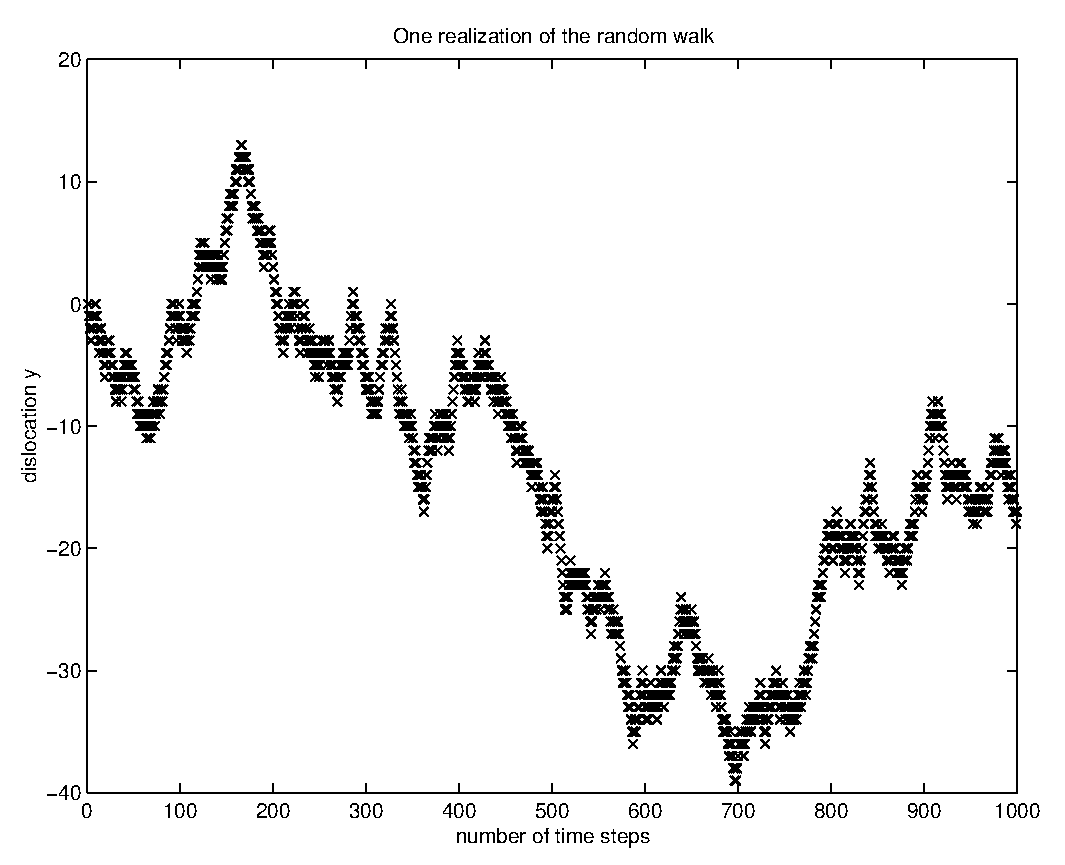
\includegraphics[width=10cm]{./Figures/f_rwdt_2.eps}
\caption{Another realization of a one--dimensional random walk.}
\end{figure}

In order to check the theoretical prediction that the mean square
displacement is proportional to the number of steps we generalize the program
{\sf rwdt} to allow for the generation of more realizations and 
the estimation of the mean value and variance. The new program is called 
{\sf rwdtn} and generates {\sf nreal} realizations of the 
stochastic process.
Its listing can be seen below.

\subsubsection{Listing of the program rwdtn.m}
\inputlisting{./Listings/rwdtn.m}
We run the program for $nstep=100$ and $nreal=1000$. The estimated
mean value of 0.274 and the estimated variance of 103.304 are in quite
good agreement with the theoretical expected vales of 0 nd 100, respectively.
It is interesting to look also at the distribution of the end points of 
the random walk. This can be seen in Fig. (\ref{F_RWDTN}).
\begin{figure}
\label{F_RWDTN}
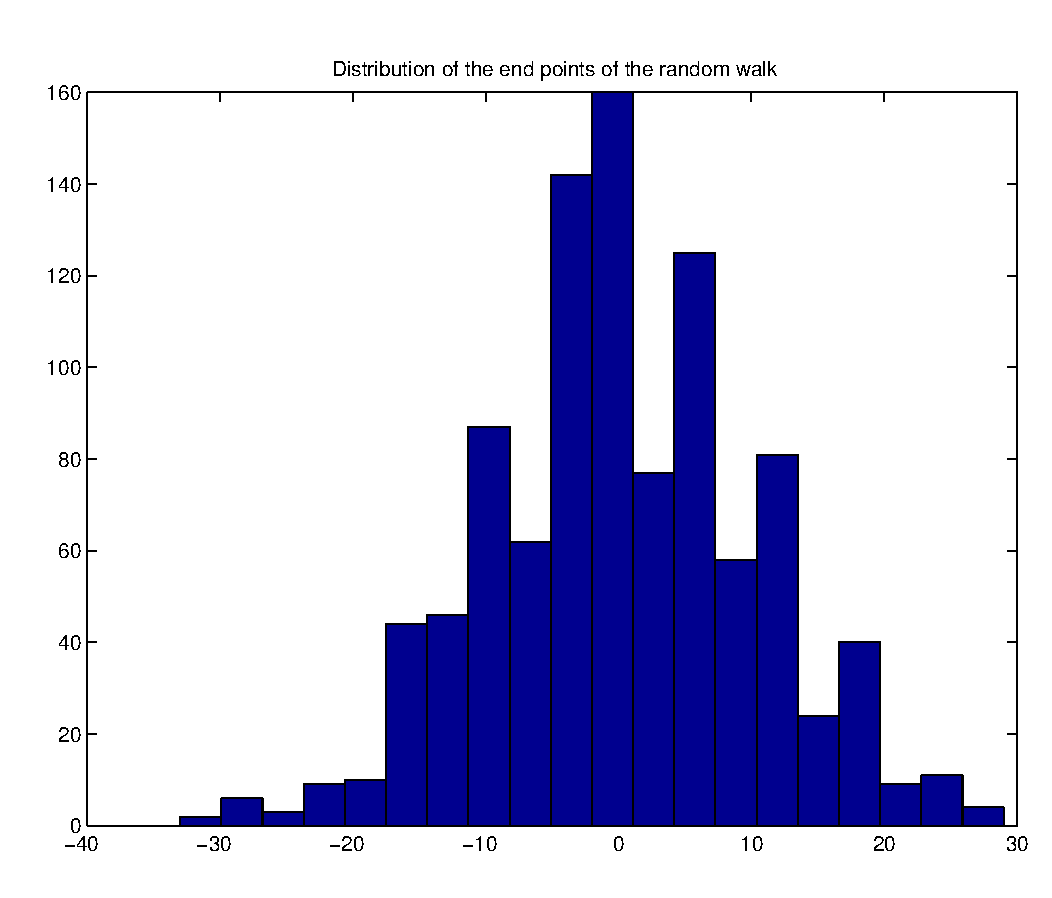
\includegraphics[width=10cm]{./Figures/f_rwdtn.eps}
\caption{The distribution of the end--points of the one--dimensional 
random walk. the program {\sf rwdtn} was run for nstep=100 and 
nreal=1000.}
\end{figure}
\subsection{Generation of Gaussian random numbers}
As a simple demonstration of the central limit theorem we want to 
generate Gaussian distributed random numbers by adding uniformly 
distributed ones.

We know that uniformly distributed random numbers on the interval
$[0,1)$ have $p(x) =1$ for $x\in[0,1)$. Then it is easy to show 
that 
\begin{equation*}
\langle X\rangle = \frac{1}{2}
\end{equation*}
and
\begin{equation*}
{\rm Var}(X) = \int_0^1 x^2 dx - \langle X^2\rangle = \frac{1}{3} 
        -\frac{1}{4} = \frac{1}{12}.
\end{equation*}
Now let us consider the transformed random variable $X'$
\begin{equation*}
X' = (X - \frac{1}{2})\sqrt{12} \sigma
\end{equation*}
which has mean $0$, variance $\sigma^2$, and is uniformly 
distributed on the interval 
$[-\frac{1}{12} \sqrt{12} \sigma, \frac{1}{12} \sqrt{12} \sigma].$
Let us now draw $N$ such random numbers $X'_1,\ldots, X'_N$
and let us construct
the new stochastic variable $Z$
\begin{equation*}
Z= \frac{1}{\sqrt{N}} (X'_1 + \ldots + X'_N).
\end{equation*}
Then the central limit theorem states that the variable $Z$ is a Gaussian
variable with mean $0$ and variance $\sigma^2$.

With the help of the program {\sf cltgen} we want to demonstrate 
that already for $N=12$ we get Gaussian distributed random numbers
in a very good approximation.

\subsubsection{Listing of the program cltgen.m}
\inputlisting{./Listings/cltgen.m}

In Fig. (\ref{F_CLTGEN}) we see the distribution of the Gaussian 
random numbers generated with the help of the program {\sf 
cltgen}. The number of random numbers $Z$ was chosen to be 1000.
\begin{figure}
\label{F_CLTGEN}
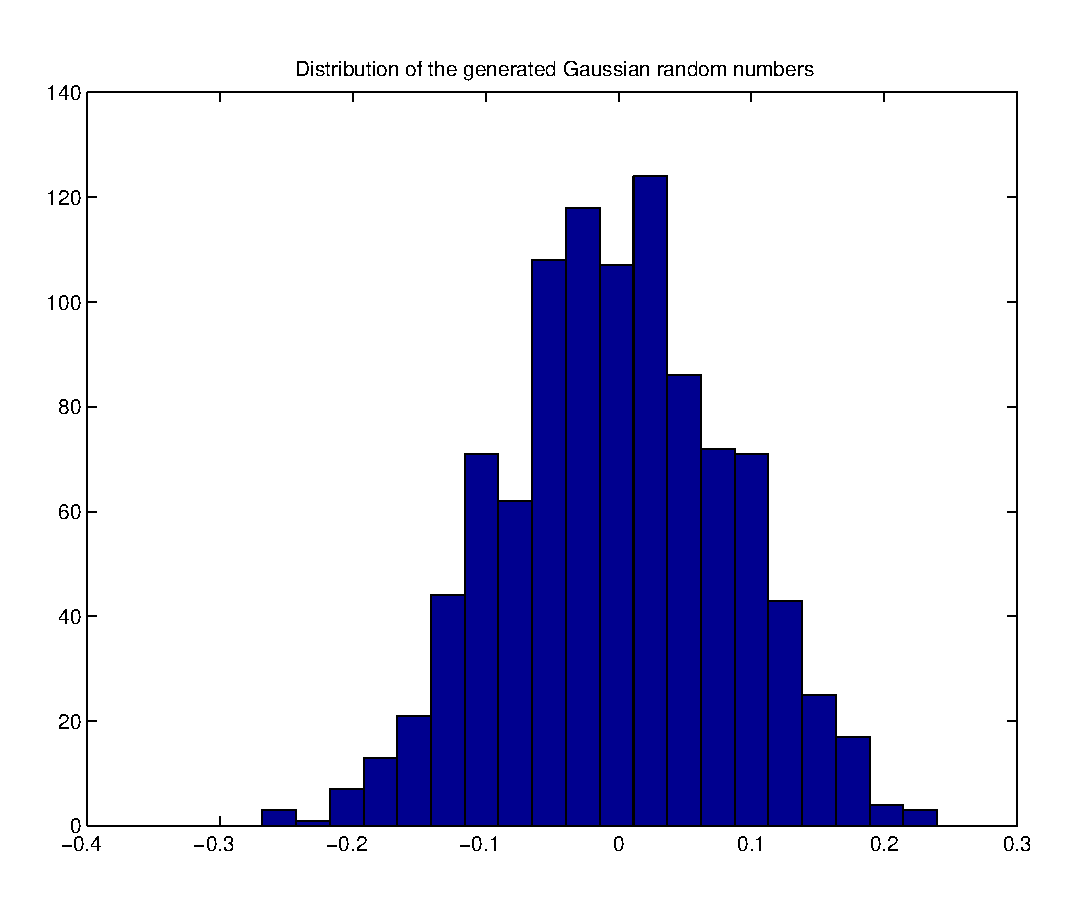
\includegraphics[width=10cm]{./Figures/f_cltgen.eps}
\caption{The distribution of the Gaussian random numbers generate
with the help of the program {\sf cltgen}. The number of random numbers 
drawn was chosen to be $n=1000$.}
\end{figure}

\subsection{Estimation}
{\em Experimental data are random numbers!} An experiment provides
realizations of some random variable $X$. We call an $N$--fold
realization of $X$ a sample of size $N$. It is of fundamental
importance to distinguish between the estimate for the mean and the
variance made on the basis of the sample, which we will denote by $m$
and by $s$, respectively and the corresponding quantities for the
(infinite) underlying population, the ensemble.

Of course, estimates should be unbiased, i.e., for very large samples
the estimate based on the sample size $N$ should converge to the
ensemble averages.

\subsubsection{Mean values}
Let us consider $N$ copies $X_1, \ldots, X_N$  of a random variable
$X$ and let us build the new stochastic variable
\begin{equation*}
Z = \frac{1}{N}(X_1 + \cdots + X_N).
\end{equation*}
$Z$ is the mean value of the $N$ realizations. Assuming that the $X_i$
are uncorrelated we obtain for the cumulants of $Z$
\begin{equation*}
\kappa_n(Z) = \frac{1}{N^n} \sum_{i=1}^N \kappa_n(X_i) =
      N^{-n+1}  \kappa_n(X).
\end{equation*}
In particular we have
\begin{eqnarray*}
\kappa(Z) & = & \langle Z \rangle = \langle X \rangle \\
\kappa_2(Z) & = & {\rm Var}(Z) = \frac{1}{N} \kappa_2(X) = \frac{1}{N}
                  {\rm Var}(X) \\
\kappa_n(Z) & = & O(N^{-2}) \;\;\; {\rm for} \;\; N>2.
\end{eqnarray*}
In other words the mean value of $Z$ is a random variable with a
distribution which has the same mean value as $X$, but with a variance
which is smaller by a factor of $N$. Up to terms of the order
$O(N^{-2})$ the distribution of $Z$ is Gaussian.

\subsubsection{Estimating mean and variance}
Let us consider to have the sample $x_1, \ldots, x_N$. A natural
estimator of the mean value $\mu$ is the sample mean
\begin{equation*}
m= \frac{1}{N} \sum_{i=1}^N x_i.
\end{equation*}
An estimate for the variance could, in analogy, naturally assumed to
be
\begin{equation*}
  \bar{\sigma}^2 = \frac{1}{N} \sum_{i=1}^N (x_i -m)^2.
\end{equation*}
Unfortunately, the above estimator is biased, because we make use of
the already known $m$ instead of the unknown $\mu$. As can easily be
seen
by adding and subtracting $\mu$ in each term in the above equation we
get
\begin {eqnarray*}
 \bar{\sigma}^2 &=& \frac{1}{N} \sum_{i=1}^N [x_i - \mu -(m-\mu)]^2 \\
                & = & \frac{1}{N} \sum_{i=1}^N (x_i - \mu)^2
                              -2(m-\mu)\frac{1}{N} \sum_{i=1}^N (x_i
                                   - \mu)
                           +(m-\mu)^2 \\
               & = & \frac{1}{N} \sum_{i=1}^N (x_i - \mu)^2 - (m-\mu)^2.
\end{eqnarray*}
Now, by taking expectation values averaging over an infinity of samples
of size $N$ we have
\begin{eqnarray*}
E[\bar{\sigma}^2] &= & E\left[\frac{1}{N} \sum_{i=1}^N (x_i - \mu)^2
                                \right]
            - E\left[(m-\mu)^2 \right] \\
       & = & \sigma^2 - \sigma_m^2.
\end{eqnarray*}
If we assume, that there are no correlations we have $\sigma^2_m=
\sigma^2/N$, an unbiased estimate of $\sigma^2$ is
\begin{equation*}
s^2 = \frac{N}{N-1} \bar{\sigma}^2 = \frac{1}{N-1} \sum_{i=1}^N 
      (x_i - m)^2.
\end{equation*}
In computations, if the sample is large, rounding errors can be large
because $(x_i - m)$ is small. In
these cases it is convenient to use the 
"corrected two--pass algorithm" for $s^2$
\begin{equation*}
s^2 = \frac{1}{N-1} \left\{ \sum_{i=1}^N 
      (x_i - m)^2 - \frac{1}{N} \left[\sum_{i=1}^N 
      (x_i - m) \right]^2  \right\}.
\end{equation*}
The function of the additional second term which would be identically
equal to zero if $m$ were exact is to correct the rounding errors of
the first term \cite{PRESS}.

\subsubsection{Confidence levels}
It is important to have also a quantitative characterization of the
goodness of the estimation. To this end we assign to every 
estimation a certain confidence interval, which is to be chosen in 
such a way that the true value lies within this interval at some
predetermined level of confidence. Since we know, by virtue of the
central limit theorem, that the mean value is Gaussian distributed
a criterion for the error can be directly derived from the 
geometric properties of the distribution. Assuming that the
mean value is $m$ and that the standard deviation is
$\sigma_m$ then the probability to find the true value in the
interval $[m-\sigma,n+\sigma]$ is given by the surface 
under a normal probability density
between  $\mu-\sigma_m$ and $\mu + \sigma_m$
\begin{equation*}
{\rm Prob}(\mu \in [m-\sigma,n+\sigma]) =
\int_{m-\sigma}^{m+\sigma} \frac{1}{\sigma \sqrt{2\pi}}
       \exp\left( - \frac{(x-m)^2}{2\sigma^2}\right)
       = 0.683.
\end{equation*}
Thus, in $68.3 \%$ of
samples a value lying within $\pm \sigma_m$  of the population mean
$\mu$ would be found. Conversely, there is $68.3 \%$ probability that
the interval $[m-\sigma_m, m+\sigma_m]$ contains the population mean.

In general we have...

\section{Beyond this chapter}

%%%%%%%%%%%%%%%%%%%%%%%%%%%%%%%%%%%%%%%%%%%%%%%%%%%%%%%%%%%%%%%%%%
\section{Exercises}
{\bf Exercise 1} Test of the random number generator. Write a 
program which estimates the first 10 moments of rand and compare 
the result of the simulation with the expected analytical value.

{\bf Exercise 2} Random variable transformation theorem: (a) Consider 
the linear transorm of X: Y=bX+c. (b) the log--normal 
distribution.
Lit. Gillespie, Am. J. Phys. 51 (1983) 520.
lichkeitstheoretische Grundbegriffe; typische 
Verteilungen (Poisson, Gauss, Binomial); 

%%%%%%%%%%%%%%%%%%%%%%%%%%%%%%%%%%%%%%%%%%%%%%%%%%%%%%%%%%%%%%%%%%


%%% Chapter 3 
%%%%%
%%%%% Chapter 3
%%%%%
\chapter{Simple Sampling of Probability distributions Using Random numbers}
This Chapter is devoted to the following question: How can we 
generate sequences of random numbers which are distributed 
according to some given distribution?

A simple answer to this question would be to exploit some 
intrinsically random physical process. For example, one could 
record a sequence of the decay times of some radioactive substance 
and use this truly random sequence of numbers in a Monte--Carlo
simulation. Although tables of millions of such true random 
numbers exist in practice this approach turns out not to be very
practical. Monte--Carlo simulations need very long sequences of 
random numbers, so that we have to find more efficient ways to 
generate them. In order to satisfy this requirement we have to 
be satisfied with the use of so--called pseudo--random numbers.
Pseudo--random numbers are generated numerically with the help of 
some simple algorithm on some computer. Consequently, they are
reproducible. This is, however, not a drawback. In fact, the 
reproducibility may be very useful if we want to check our 
simulation algorithms. 

Pseudo--random numbers are, the name already underlines it, not 
truly random. However, their statistical properties are very 
similar to the statistical properties of truly random numbers. So, 
for all practical purposes pseudo--random numbers appear to be 
random. Let us now see how such pseudo--random numbers can be 
generated.

\section{The generation of uniformly distributed random numbers}
We will begin with the generation of uniformly distributed random 
numbers on the interval $[0,1)$. In the following we will often 
omitt the prefix pseudo. 

The best known algorithm for the generation of uniformly 
distributed random numbers is the linear congruential method, 
which given an initial integer "seed" value $I_1$ produces random 
integers recursively from the formula
\begin{equation*}
I_{n+1} = (aI_n +c) \mod M,
\end{equation*}
where $a$, $c$, and $M$ are integer constants which have to be 
chosen appropriately. 
The randomness of the above algorithm results from the fact that 
after some multipications with $a$ the result exceeds $M$ and is 
consequently truncated. Since the integers $I_n$ lie between 1 and 
$M$ a random number $R$ uniformly distributed 
between 0 and 1 is obtained as
\begin{equation*}
R = \frac{I_n}{M}.
\end{equation*}
Unfortunately, MATLAB does not have integer arithmetic so the above algorithm 
has to be implemented using the {\sf rem} (remainder) function 
instead of the modulo function. A corresponding code could be
\begin{verbatim}
I(n+1) = floor( rem(a*I(n) + c,M) ).
\end{verbatim}
In order to get familiar with this algorithm we want to generate a 
sequence of pseudo--random numbers for the following parameters:
we choose the multiplier to be $a=$, the increment $c=3$, and the 
modulo $M=8$. Obviously the longest period of random numbers will
have the length 8. The generation of the random sequences will
be achieved with the program {\sf trandom1}.

\subsubsection{Listing of the program trandom1.m}
%%%%% trandom1 %%%%%%%%%%%%%%%%
\begin{verbatim}
% trandom1 - Program to demonstrate the generation of random numbers
% using the linear congruential method
clear; help trandom1 %clear the memory and print header
seed = input('Enter the seed (1) - ');
m = input('Enter the modulus (8) - ');
a = input('Enter the multiplier (5) - ');
c = input('Enter the increment (1<=c<7) - ');
% Set starting value
R(1) = seed;
% Generate vector of m random numbers
for j=1:m
   R(j+1) =floor(rem(a*R(j)+c,m));
end
%R=R/M;
disp('The generated series is:')
disp(R)
plot(R,'x')
title('The series of generated random numbers');
xlabel('Term, i'); ylabel('Value');
\end{verbatim}
%%%%%%%%%%%%%%%%%%%%%%%%%%%%%%%%%%%%%%%%%%%%%%%%%%%%%%%%%%%%%%%

Run with the above parameters the program generates the sequence
\begin{equation*}
1, 0, 3, 2, 5, 4, 7, 6, 1, 0, 3, 2 \ldots
\end{equation*}
which has also been plotted in Fig. (\ref{F_TRANDOM1}).
\begin{figure}
\label{F_TRANDOM1}
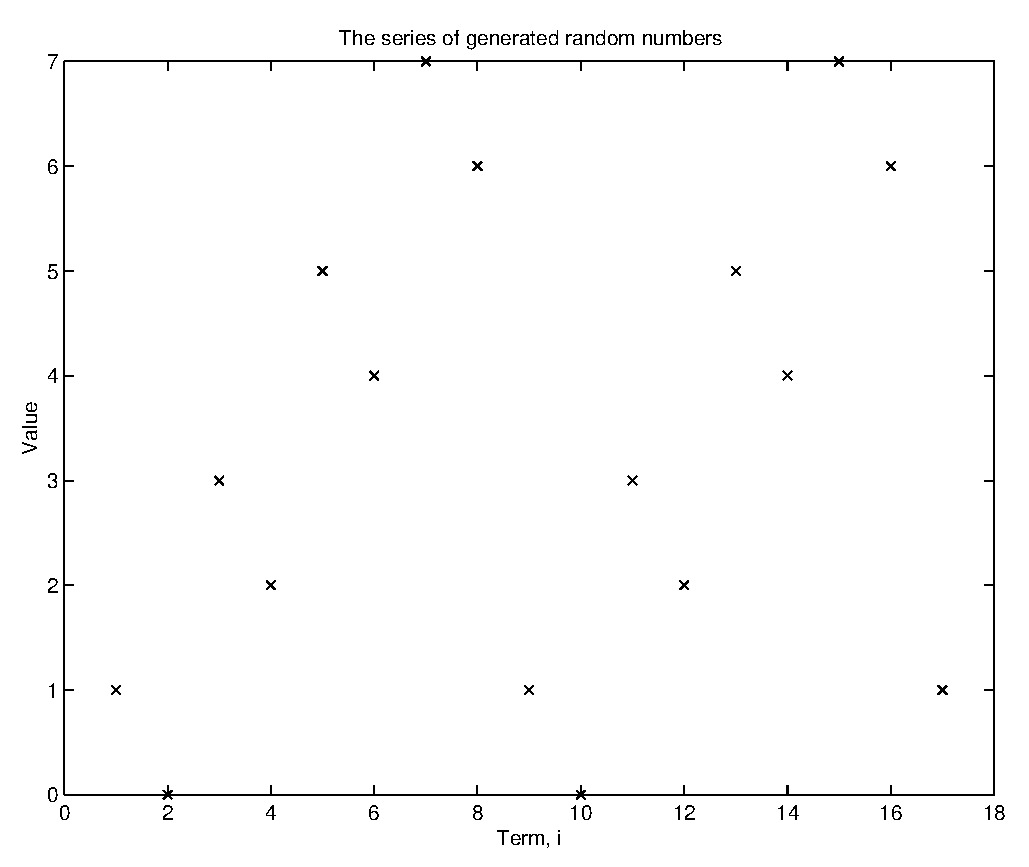
\includegraphics[width=10cm]{./Figures/f_trandom1.eps}
\caption{Successive values in a series of random numbers generated
for a=5, c=3, M=8. Note that the even numbers are always one less 
then the odd ones!}
\end{figure}
It might be instructive to run the program keeping the multiplier 
and the modulo fixed while changing the increment. The result of 
these runs are summarized in Table \ref{T_LCG}.

\begin{table}
\label{T_LCG}
\caption{Series of random numbers for the linear congruential 
generator of the form $I_{n+1} = (5I_n +c) \mod 8$}
\begin{tabular}{ccc} \hline
c &  $I_n$ & Period  \\ \hline
1 & 1,6,7,4,5,2,3,0 & 8 \\
2 & 1,7,5,3,1,7,5,3 & 4 \\
  & 4,6,0,2,4,6,0,2 & 4 \\
3 & 1,0,3,2,5,4,7,6 & 8 \\
4 & 1,1,1,1,1,1,1,1 & 1 \\
  & 2,6,2,6,2,6,2,6 & 2 \\
  & 3,3,3,3,3,3,3,3 & 1 \\
  & 4,0,4,0,4,0,4,0 & 2 \\
  & 5,5,5,5,5,5,5,5 & 1 \\
  & 7,7,7,7,7,7,7,7 & 1 \\
5 & 1,2,7,0,5,6,3,4 & 1 \\
6 & 1,3,5,7,1,3,5,7 & 4 \\
  & 2,0,6,4,2,0,6,4 & 4 \\
7 & 1,4,3,6,5,0,7,2 & 8
\end{tabular}
\end{table}
It is evident that a wrong  choice of the constants leads to a 
very poor random sequence.

It can be shown that (Knuth)  that in the case $c=0$ the full 
period, 1 to $M-1$ can be achieved by choosing $M$ as aprime 
number and for $a$, a primitive element modulo $m$, i.e., for all 
prime divisors, $p$, of $(M-1)$, 
\begin{equation*}
a^{(M-1)/p} {\rm mod} M \ne 1.
\end{equation*}
For the case of $c\ne 0$ the full period is obtained if the 
following three conditions are satisfied:

(i) $c$ and $M$ are relatively prime,

(ii) $a {\rm mod} p = 1$ for each prime factor $p$ of $M$,

(iii) $a {\rm mod} 4 = 1$ if 4 divides $M$.

It is evident that the greater the modulus the longer the period.
For example the MATLAB random number generating function uses
\begin{equation*}
a= 16807; c=0; M=2^{31}-1.
\end{equation*}
This chioce has been suggested by Park and Miller (Lit. Press).
The period of the generator is $2^{31}-2 \approx 2.1 \times 10^9$.
Another poupular popular random generator uses
\begin{equation*}
a= 65539; M=2^{31}-1; c=0,
\end{equation*}
and will be used in the following program {\sf trandom2.m}. There 
we will draw a number $n=xxx$ of random numbers using the linear 
congruential method. In the program we will check the quality of 
the generator by plotting the 1D, 2D, and 3D distribution of the 
pseudo--random numbers. The results of the test can be seen in 
Figs. (\ref{F_TRANDOM2_1}), (\ref{F_TRANDOM2_2}), 
(\ref{F_TRANDOM2_3}), and (\ref{F_TRANDOM2_4}).



\subsubsection{Listing of the program trandom2.m}
\begin{verbatim}
% trandom2 - Program to test random number generators
% The program makes use of the random number generator random1
clear; help trandom2; % clear memory and print header
% Enter dimension of random vector
n= input('Enter value of n-'); % 
% generate random vector
R1=random1(n);
% plot random vector
plot(R1)
title('random numbers'); xlabel('random variable');
disp('Histogram: press any keyboard key');
pause;
% plot histogram of random numbers
x=(0.05:0.1:0.95);
[m,xout] = hist(R1,x);
bar(xout,m)
xlabel('random number');
title('1D distribution: Histogram');
disp('2D plot: press any keyboard key');
pause;
% 2D plot: correlation of consecutive numbers
R2x=R1(1:2:n-1);
R2y=R1(2:2:n);
plot(R2x,R2y,'x')
title('2d distribution')
disp('3D plot: press any keyboard key');
pause;
% 3D plot: correlation of consecutive numbers
R3x=R1(1:3:n);
R3y=R1(2:3:n);
R3z=R1(3:3:n);
%R3=random1(n,3);
plot3(R3x,R3y,R3z,'x')
title('3D distribution');xlabel('Random number');
\end{verbatim}

\subsubsection{Listing of the function {\sf random1}}
%%%%%%%%%%%%%%%%%%%%%%%%%%%%%%%%%%%%%%%%%%%%
\begin{verbatim}
function R = random1(n)
% function to generate random numbers
a=65539;
M=2^(31)-1;
R(1) = 12345678;
for j=1:n-1
%   for i=1:n-1
   R(j+1) =floor(rem(a*R(j),M));
%end
end
R=R/M;
\end{verbatim}

\begin{figure}
\label{F_TRANDOM2_1}
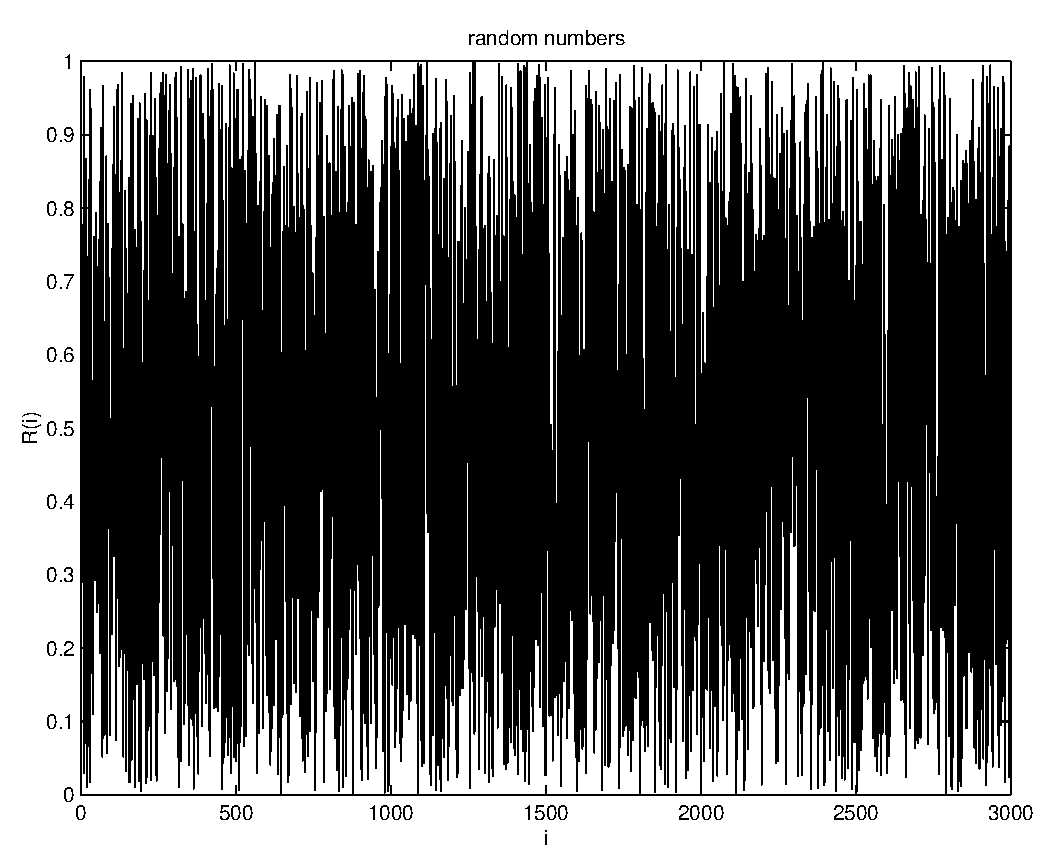
\includegraphics[width=10cm]{./Figures/f_trandom2_1.eps}
\caption{Successive values in a series of 3000 random numbers generated
for $a=65539$, $c=0$, $M=2^{31}-1$.}
\end{figure}

\begin{figure}
\label{F_TRANDOM2_2}
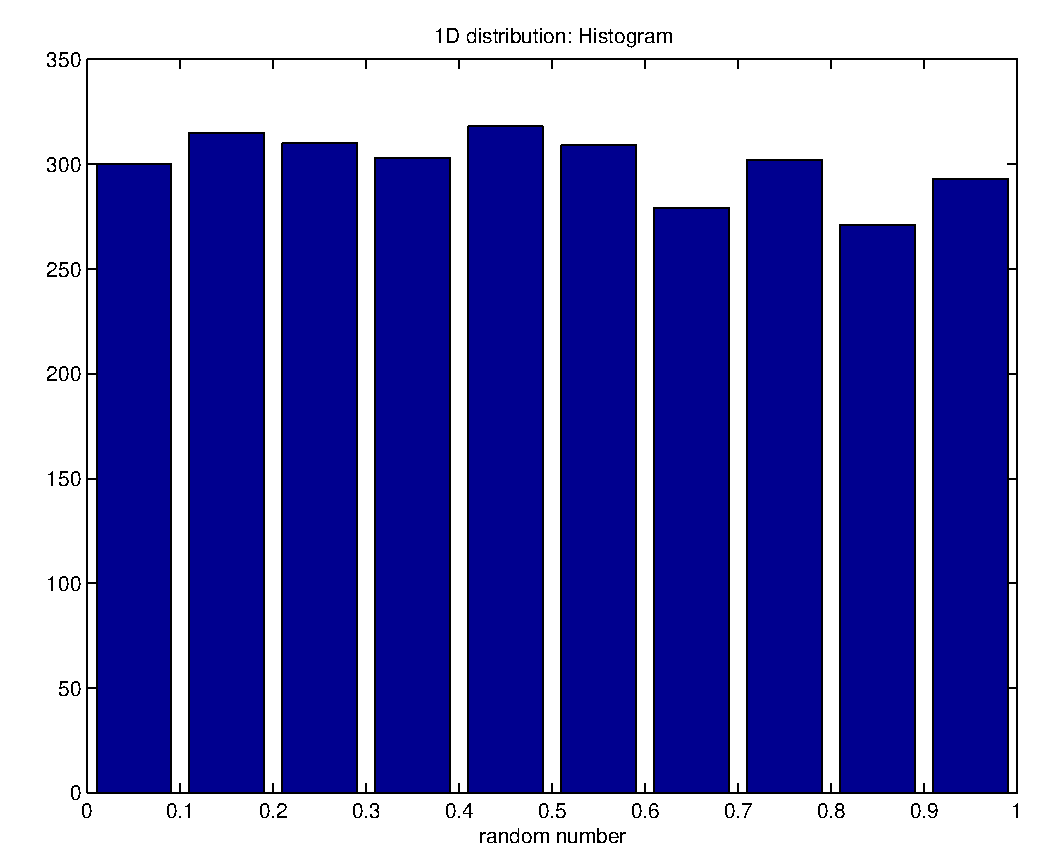
\includegraphics[width=10cm]{./Figures/f_trandom2_2.eps}
\caption{Histogram for a series of 3000 random numbers generated
for $a=65539$, $c=0$, $M=2^{31}-1$.}
\end{figure}

\begin{figure}
\label{F_TRANDOM2_3}
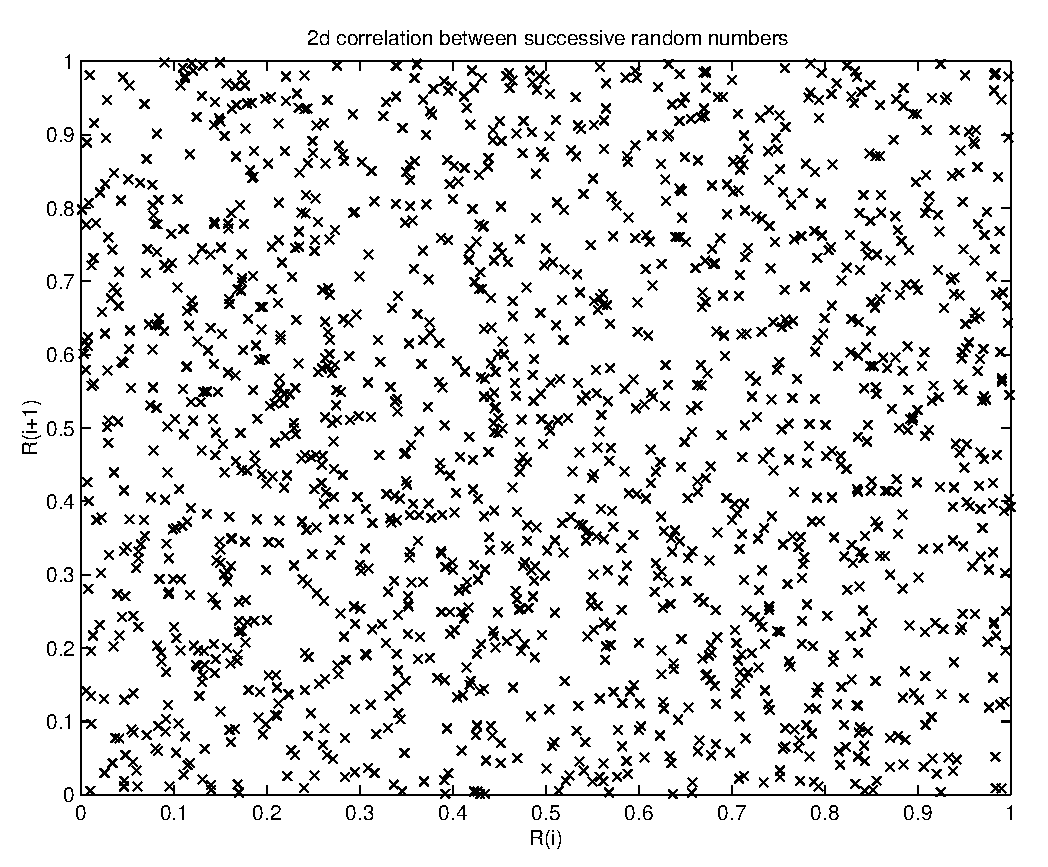
\includegraphics[width=10cm]{./Figures/f_trandom2_3.eps}
\caption{Correlation between successive values in a series of 3000 
random numbers generated for $a=65539$, $c=0$, $M=2^{31}-1$.}
\end{figure}


\begin{figure}
\label{F_TRANDOM2_4}
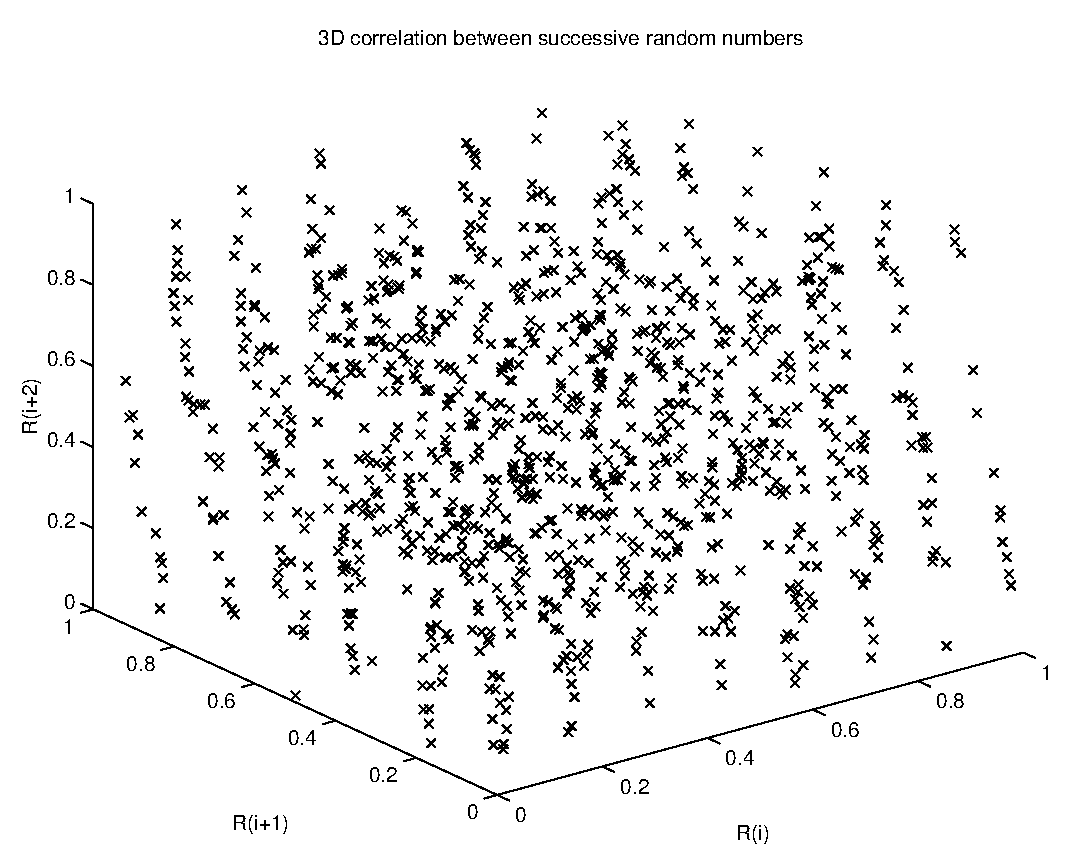
\includegraphics[width=10cm]{./Figures/f_trandom2_4.eps}
\caption{Correlation between successive values 
$R(i),R(i+1), R(i+2)$ in a series of 3000 random numbers generated
for $a=65539, c=0, M=2^{31}-1$.}
\end{figure}

The figures clearly reveal that the generator is not perfect.
In the exercise we will learn that choosing $a=16807$, the minimal
standard generator, 
significantly improves the performance. The performance of 
this minimal standard generator can be increased by shuffling
the output to remove low--order serial correlations (EXERCISE!!!!)
({\sf ran1} of Numerical Recipes).

In the book by Press et al. other "Quick and Dirty" linear 
congruential generators
are presented. Furthemore, serial correlations can be broken up by 
combining two linear congruential generators.

There are also other algorithms for the generation of random 
numbers: Shift--register generators (Lit: Kirkpatrick and Stoll), 
Fibonacci generators (lit: Knuth, James) or quasi--random numbers 
and we refer the reader to the original literature.

\section{The Transfomation method: Invertible distributions}
In the previous section we have learned how to generate random 
numbers with a uniform probability distribution, so that the 
probability $p(x)dx$ to generate a random number between $x$ and $x+dx$
is given by
\begin{equation*}
P(x)dx = \left\{ \begin{array}{ll}
                   dx & 0<x<1 \\
                   0   & {\rm otherwise}.
                  \end{array}
         \right.
\end{equation*}
With the help of the random variable transformation theorem it is easy
to transform uniform deviates into random numbers which are 
distributed according to invertible, one--to--one, distributions.
We know from Chap. 2 that if we take a uniform deviate $x$ and then 
transform it to a new variable $y(x)$ the probability distribtion
of $y$ is given by
\begin{equation}
p(y) = p(x) \left| \frac{dx}{dx}\right|.
\end{equation}
We want to derive a transformation which generates random numbers 
which are distributed according to a given
$p(y)$. Since $x$ is uniformly distributed the 
above equation reduces to
\begin{equation}
\label{INVERTIBLE}
\frac{dx}{dy} = p(y),
\end{equation}
which can be easily integrated
\begin{equation*}
x(y) = P(y) = \int^y p(y')dy'.
\end{equation*}
Hence, the transformation we are looking for is given by the 
inverse of $P(y)$. Thus, a random variable $Y$ with density $p(y)$
can be generated by uniform deviates trough
\begin{equation*}
Y = Y(X) = P^{-1}(X).
\end{equation*}
In the following we will apply this method to generate 
exponentially and gaussian distributed random numbers.

\subsection{Exponential distribution}
Let $p(y)= w\exp(-wy)$ for positive $y$. It follows from Eq. (\ref{INVERTIBLE})
that
\begin{equation*}
\frac{dx}{dy} = w \exp(-wy).
\end{equation*}
Therefore we get immediately
\begin{equation*}
x(y) = \int_0^{\infty} dy'w\exp(-wy') = 1-\exp(-wy).
\end{equation*}
The above expression is easily inverted
\begin{equation*}
y=-\frac{1}{w}\ln(1-x),
\end{equation*}
and since $x$ is equally distributed in $[0,1]$ we can generate 
exponentially distributed random numbers with the help of the 
formula
\begin{equation}
y = - \frac{1}{w} \ln(x).
\end{equation}
It is clear that in MATLAB such an exponentially distributed 
random number $Y$ can be generated with the help of the following 
line of code
\begin{verbatim}
y = - log( rand(1) )/w
\end{verbatim}
With the help of the simple program {\sf expdistr} we want to 
generate 1000 exponentially distributed random numbers and compare
them with the prescribed distribution. We check also the mean 
value and variance and compare them with the analytical expectation 
values.

\subsubsection{Listing of the program expdistr.m}

In Fig. (\ref{F_EXPDISTR}) we see the histogram of 1000 drawn exponentially 
distributed random numbers.
\begin{figure}
\label{F_EXPDISTR}
\includegraphics[width=10cm]{./Figures/f_expdistr.eps}
\caption{Histogram of 1000 exponentially distributed random numbers with
mean 1 generated according to the transformation method. The continuous
line represents the expected exponential distribution.}
\end{figure}

\subsection{Gaussian distributed random numbers}
Gaussian distributed random numbers can be obtained with the help 
of the multidimensional random variable transformation theorem.
Let us consider the transformation
\begin{eqnarray}
\label{GAUSS-GEN1}
y_1 & = & \sqrt{-2\log(x_1)} \cos(2 \pi x_2) \\
\label{GAUSS_GEN2}
y_2 & = & \sqrt{-2\log(x_1)} \sin(2 \pi x_2),
\end{eqnarray}
where $X_1$ and $X_2$ are uniformly distributed random numbers on 
the interval $[0,1)$. Equivalently we can write
\begin{eqnarray*}
x_1 & = & \exp[-\frac{1}{2}(y_1^2+y_2^2)] \\
x_2 & = & \frac{1}{2 \pi} \arctan\left( \frac{y_1}{y_2}\right).
\end{eqnarray*}
it is now straightforward  to show that the Jacobian determinant
reads
\begin{equation*}
\frac{\partial(x_1,x_2)}{\partial(y_1,y_2)} = 
   - \left[ \frac{1}{\sqrt{2 \pi}} \exp(-y_1^2/2)\right]
   \left[ \frac{1}{\sqrt{2 \pi}} \exp(-y_2^2/2)\right].
\end{equation*}
The right hand side of the above equation corresponds to the 
product of two independent Gaussian distributions. Thus it follows
from the multidimensional version of the random variable 
transformation  theorem for invertible distributions that the
two random number generated according to Eqs. (\ref{GAUSS-GEN1}) 
and (\ref{GAUSS-GEN2}) are Gaussian distributed. This algorithm 
which allows the generation of two Gaussian random numbers from 
two uniformly distributed ones is called the Box--Muller method.

It is clear that it easy to implement the above algorithm in 
MATLAB. This is done in the program {\sf gaussdistr.m} which generates
gaussian random numbers with mean value $mu$ and variance $sigma$.

\subsubsection{Listing of the program gaussdistr.m}

The corresponding histogram obtained by running the program for
n=1000, mu=0, sigma=2 can be seen in Fig. (\ref{F_GAUSSDISTR}).
\begin{figure}
\label{F_GAUSSDISTR}
\includegraphics[width=10cm]{./Figures/f_gaussdistr.eps}
\caption{Histogram of 1000 Gaussian distributed random numbers with
mean 0 and variance 2 generated according to the Box-Muller method. 
The continuous line represents the expected Gaussian density.}
\end{figure}

Let us end this subsection by mentioned that normal distributed
random numbers can be generated in MATLAB with the help of 
the function {\sf randn}.

\section{The acceptance--rejection technique}
The acceptance--rejection technique is a method of wide 
applicability. In its original formulation it is due to 
von--Neumann. The basic idea is to sample a random number
from some known and appropriate probability distribution and to 
perform a test to determine whether or not it is acceptable for 
use or not. We follow Rubinstein but consider for simplicity only
the one--dimensional case.

Let us assume that the stochastic variable $X$ is defined on the 
interval $a \le x \le b$ and is distributed according to the
probability density $p(x)$. We write this probability distribution 
as
\begin{equation*}
p(x) = C d(x) q(x),
\end{equation*}
where $C$ is a normalization constant $C \ge 1$, $q(x)$ is also a 
probability distribution and $0 \le d(x) \le 1$. The probability 
distribution $q(x)$ is the importance function, and  we are 
supposed to know how to generate random variates distrubuted 
according to it.

The accepatnce--rejection method works as follows. We generate two
random variates, $\xi$ is uniformly distributed on the interval
$[0,1)$ and $Y$ is distributed according to $q(y)$. Then we test
whether or nor the equality
\begin{equation*}
\xi \le d(y)
\end{equation*}
holds or not. If  the conditione $\xi \le d(y)$ is satisfied, 
then $Y$ is accepted as 
a random variate distributed according to $p(x)$.  If
the condition is not satisfied, the pair $(\xi,y)$ is rejected, 
and we have to try again.

It is easy to demonstrate that the above methd works. Let us apply
Bayes'formula to the conditional probability $p(x|\xi \le d(y)$:
\begin{equation}
\label{A-R-BAYES}
p(x|\xi \le d(y) = \frac{{\rm Prob}(p(x|\xi \le d(y)|Y=x)q(x)}
                  {{\rm Prob}(\xi \le d(y))}.
\end{equation}
It is straightforward to compute
\begin{eqnarray*}
{\rm Prob}(p(x|\xi \le d(y)|Y=x) &=& {\rm Prob}(\xi \le d(x)) = 
          d(x) \\
{\rm Prob}(\xi \le d(y)) & = & \int {\rm Prob}(\xi \le d(Y|Y=x)) q(x) dx \\
               &= & \int q(x) d(x)dx = \int dx \frac{p(x)}{C} = 
                   \frac{1}{C}.
\end{eqnarray*}
Inserting into (\ref{A-R-BAYES}) we obatin finally
\begin{equation*}
p(x|\xi \le d(y) = p(x),
\end{equation*}
which completes the proof.

The above discussion also makes evident the role of the constant
$C$. The efficiency of the method depends on the inequality $\xi \le 
d(y)$, for independent trials the probability of success is given 
by $1/C$. $C$ represents the average number of passes which must 
be made with the algorithm in order to select a variate. It is 
clear, that in order for the method to be efficient it must be 
easy to generate random numbers according to $q(x)$ and the 
efficiency should be large, i.e., $C$ should be close to one.

In the original formulation by von--Neumann the comparison 
function was simply chosen to be the uniform distribution. If
$M$ is the maximum of $p(x)$ then we choose
\begin{eqnarray*}
q(x) & = & \frac{1}{b-a} \\
d(x) & = & \frac{p(x)}{M} \\
C & = & M(b-a).
\end{eqnarray*}
The von--Neumann algorithm then simply reads \\
1. Generate $\chi_1$ and $\chi_2$ uniformly distributed in 
    $[0,1)$. \\
2. Evaluate $Y=a+\chi_2(b-a)$. \\
3. If $\chi_1 \le p(x)/M$ then $Y$ is a variate distributed 
    according to $p(x)$. \\
4. Go to 1.

As a simple example we want to generate random numbers on $[0,1)$    
distributed according to
\begin{equation*}
p(x) = 3x^2; \;\;\; 0 \le x <1.
\end{equation*}
We choose $C=3$ and apply the von--Neumann algorithm. \\
1. Generate $\chi_1$ and $\chi_2$ uniformly distributed in 
    $[0,1)$. \\
2. Test the inequality $\chi_1 \le \chi_2^2.$     \\
3. If the equality holds we accept $\chi_2$ as a random number 
generated according to $p(x)$.

The above algorithm has been implemented in MATLAB in the program
{\sf neumann.m}, which we run for $n=1000$ and $n=5000$. The 
result of the latter run can be seen in Fig. (\ref{F_NEUMANN}).
\begin{figure}
\label{F_NEUMANN}
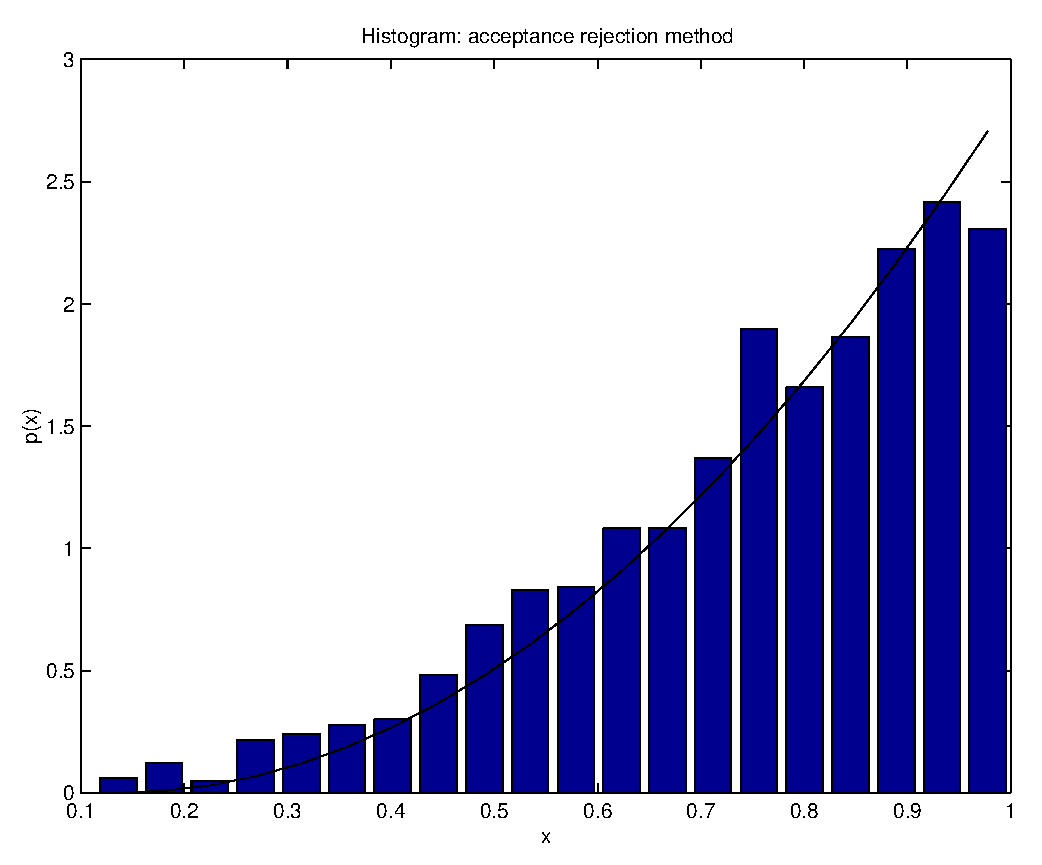
\includegraphics[width=10cm]{./Figures/f_neumann.eps}
\caption{Histogram of 5000 random numbers distributed
according to $p(x) = 3x^2$ generated with the von--Neumann
acceptance--rejection technique.
The continuous line represents the exact density $p(x)$.}
\end{figure}
In the program we count the number of successful trials. The ratio
of successful trials to the total number of drawn random pairs for 
the run shown
is 0.3328, which is in good agreement we the expected theoretical
value of $1/C=1/3$.

\subsubsection{Listing of the program neumann.m}




%\subsection{Poisson distributed random numbers}

\section{Variance reduction: Importance Sampling}
In this section we will see how the Monte--Carlo integration
algorithms can considerably be improved. The importance sampling 
technique will be our first encounter with a so--called variance 
reduction technique. We already know that the estimation of 
integrals by the Monte--Carlo method is affected with errors. The
basic idea of variance reduction techniques is to use known 
informations about the problem in order to improve the efficiency 
of the simulation. Obviuosly, if nothing is known about the 
problem no variance reduction can be achieved. On the other 
extreme, if we have full knowledge the variance will be reduced to 
zero, and there will be no need for a simulation. It is always 
important to be aware of what is known about the system.

We now consider the problem of estimating the integral
\begin{equation}
\label{INT_VARRED}
I = \int dx f(x).
\end{equation}
The central idea of importance sampling is to select random 
variates from regions in proportion to the importance these 
regions make to the integral we want to evaluate, instead of 
spreading them evenly. To this end we rewite the integral 
(\ref{INT_VARRED}) in the form
\begin{equation*}
I = \int \frac{f(x)}{p(x)} p(x) dx = \langle 
\frac{f(x)}{p(x)}\rangle,
\end{equation*}
where $X$ is a random variable with probability density $p(x)$.
$P(x)$ is called the importance sampling distribution.  Since the
integral is obviously the expectation value of the function $f(x)/p(x)$
it can be estimated using $N$ random numbers $X_i$ distributed 
according to $p(x)$
\begin{equation*}
\hat{I}_N = \frac{1}{N} \sum_{i=1}^N \frac{f(x_i)}{p(x_i)}.
\end{equation*}
The function $p(x)$ has to be chosen in such a way that the 
variance of $f(x)/p(x)$ 
\begin{equation*}
{\rm Var} = \langle (\frac{f(x)}{p(x)}-I)^2\rangle
   = \int_a^b \frac{f^2(x)}{p(x)}dx - I^2
\end{equation*}
is minimal. If $f(x)>0$ it follows from the above equation that
${\rm Var}=0$ if we choose $p(x)$ as $p(x) = f(x)/I$. 
Unfortunately, this choice implies that we have to know already 
the integral we want to solve. In general, the variance can 
essentially be reduced if $p(x)$ is chosen to resemble $f(x)$.

As an example we consider the integral
\begin{equation}
\label{I_MCI_IS}
I= \int_0^1 dx \exp(-x^2).
\end{equation}
In the first two columns of table (\ref{T_MCI_IS}) we show
the results of two estimates of the above integral with the 
help of the standard Monte--Carlo integration. In the third column 
we show the results of the importance sampling integration.

\begin{table}\label{T_MCI_IS}
\caption{Monte--Carlo estimates of the integral (\ref{I_MCI_IS})
using the standard method $p(x)=1$ and the importance sampling method
$p(x)=a\exp(-x)$}
\begin{center}
\begin{tabular}{llll}
 ~             & $p(x) =1$ & $p(x) =1$ & $p(x)=a\exp(-x)$ \\ \hline
$N$            & 1000      & 16384      & 1000           \\
$I$            & 0.736087  & 0.74504    & 0.748340        \\
$\sigma_I$     & 0.00131   & 0.000317   & $9.65 \times 10^{-5}$ \\
CPU time/trial (s) & 0.000660  & 0.003837   & 0.000860  \\
total CPU time (s) & 0.66      & 62.86      & 0.86 
\end{tabular}
\end{center}
\end{table}
The simulation was performed with the help of the program
{\sf mciis.m} whose listing can be seen below.

\subsubsection{Listing of the program mciis.m}
%\includelistings{.\Listings\mciis.m}

The importance sampling function is chosen to be $p(x)=a\exp(-x)$,
where the constant $a$ is chosen such that $p(x)$ is normalized
on the  unit interval. Accordingly the $N$ random numbers $X_i$
distributed according to $p(x)$ are generated with the help of the
inversion method. Since
\begin{equation*}
P(x) = \int_0^x dx' p(x') = a[1-\exp(-1)]
\end{equation*}
the exponentially distributed random numbers on the interval $[0,1)$
are generated according to
\begin{equation*}
X = - \log(1- \chi/a),
\end{equation*}
where the $chi$ are uniformly distributed random numbers on the 
interval $[0,1)$. The generation of these random numbers is 
performed in lines x to y.

It is important to remark that although the computation time per
trial is larger in the importance sampling technique the total CPU 
time is smaller compared to the standard Monte Carlo algorithm 
because a much smaller number of realizations is required in order
to achieve a desired accuracy (variance).





\section{Self--Avoiding random walks}
\subsection{Simple sampling}
\subsection{Importance sampling}
%%%%%%%%%%%%%%%%%%%%%%%%%%%%%%%%%%%%%%%%%%%%%%%%%%%%
%%%%%%%%%%%%%%%%%%%%%%%%%%%%%%%%%%%%%%%%%%%%%%%%%%%%%
%%%%%%%%%%%%%%%%%%%%%%%%%%%%%%%%%%%%%%%%%%%%%%%%%%%%%
%%%%%%%%%%%%%%%%%%%%%%%%%%%%%%%%%%%%%%%%%%%%%%%%%%%%%
%%%%%%%%%%%%%%%%%%%%%%%%%%%%%%%%%%%%%%%%%%%%%%%%%%%%%
%%%%%%%%%%%%%%%%%%%%%%%%%%%%%%%%%%%%%%%%%%%%%%%%%%%%%
%%%%%%%%%%%%%%%%%%%%%%%%%%%%%%%%%%%%%%%%%%%%%%%%%%%%%
\chapter{Stochastische Prozesse}
Master-Gleichungen

\chapter{Monte Carlo Methoden in der statistischen Mechanik}
Metropolis; Ising; Finite-Size Effects; Random Walks; SAW (?)
Simulated annealing; travelling salesman;

\chapter{Non-equilibrium MC}
Chemische Reaktionen, Diffusion; Reaktions-Diffusion, Turbulenz.

\chapter{Brownsche Dynamik Simulationen}
Omega-entwicklung; SDE;


\chapter{Rest}
stochastische Resonanzen; Muster Erkennung; random Walks;

\chapter{Stochastische Wellenfunktionsmethoden}


%%% Chapter 4 
\chapter{Stochastic processes and master equations}
This chapter is devoted
to the introduction of some mathematical concepts. 
We will introduce stochastic processes and we will 
see how a particular class of stochastic 
processes, the so--called Markov processes  are described 
with the help of master equations. These concepts will be applied
in the next chapters to typical examples from statistical physics.

\section{Stochastic processes}
We have already learned in Chap. 2 that once a stochastic variable 
$X$ has been defined it is possible to define other stochastic 
variables, say $Y$, as functions of $X$ by some mapping $f$. In 
particular, the quantity $Y$ may be a function of an additional
time variable $t$, i.e.,
\begin{equation*}
Y(t) = f(X,t).
\end{equation*}
Sloppy speaking, such a quantity $Y(t)$ is called a {\em stochastic
processes}. If we insert for $X$ one of its possible values $x$
we obtain an ordinary function
\begin{equation*}
y(t) = f(x,t),
\end{equation*}
which is a {\em realization} of the stochastic process. It is 
customary in statistical physics to regard the stochastic process 
as an {\em ensemble} of such realizations.

It follows immediately from the random variable transformation 
theorem that the probability density for $Y(t)$ to take the value
$y$ at time $t$ is given by
\begin{equation*}
P_1(y,t) = \int dx  \delta(y-f(x,t)) P(x)
\end{equation*}
and accordingly the joint probability density to  that $Y$ has the
value $y_1$ at time $t_1$, the value $y_2$ at time $t_2$, 
$\ldots$, and the value $y_n$ at time $t_n$ is given by
\begin{eqnarray*}
\lefteqn{P_n(y_1,t_1;y_2,t_2; \ldots, y_n,t_n)} \\
&& = \int dx \delta(y_1-f(x,t_1))\delta(y_2-f(x,t_2)) \cdots 
   \delta(y_n-f(x,t_n))  P(x).
\end{eqnarray*}
In such a way an infinite hierarchy of joint probability densities
$P_n$ $(n=1,2,\ldots)$ is defined, which allows the evaluation of 
expectation values like
\begin{eqnarray*}
\lefteqn{<Y(t_1) Y(t_2) \cdots Y(t_n)>} \\
&& = \int dy_1 dy_2 \cdots dy_n 
        y_1 y_2 \cdots y_n P_n(y_1,t_1;y_2,t_2; \ldots, y_n,t_n).
\end{eqnarray*}
It has been shown by Kolmogorov \cite{KOLMOGOROV} that the 
hierarchy of joint probability densities introduced above 
completely specifies
a stochastic process if the following four consistency conditions 
are satisfied

(i) $P_n \ge 0$; \\
(ii) $P_n$ is a symmetric function of the pairs $(y_1,t_1)$, 
$\ldots$, $(y_n,t_n)$; \\
(iii) $\int dy_n P_n(y_1,t_1; \ldots , y_n,t_n) =
     P_{n-1}(y_1,t_1; \ldots ; y_{n-1},t_{n-1})$; \\
(iv) $\int dy_1 P(y_1,t_1) =1$.

Thus, the hierarchy of joint probability densities constitutes an 
alternative way to define stochastic processes. 
With increasing $n$ the description of the stochastic processes gets
more precise. It is important to 
make the following remarks.  The condition (iii) implies that each 
density $P_n$ includes the knowledge of all previous densities
$P_k$ with $k<n$. Furthermore the density $P_n$ does have the 
following property if two time arguments are identical
\begin{equation*}
P_n(x,t;y_1,t;y_2,s_2; \ldots ; y_{n-1},s_{n-1}) = 
P_{n-1}(x,t;y_2,s_2; \ldots ; y_{n-1},s_{n-1})) 
\delta(x-y_1).
\end{equation*}
The hierarchy of probability densities is also the starting point 
for the classification of stochastic processes. A stochastic 
process is said to be purely random if events at different times 
are not correlated. In this case the joint probability density 
factorizes, i.e. we have
\begin{eqnarray*}
P_2(y_1,t_1;y_2,t_2) &=& P_1(y_1,t_1) P_1(y_2,t_2) \\
P_3(y_1,t_1;y_2,t_2;y_3,t_3) &=& P_1(y_1,t_1) P_1(y_2,t_2)P_1(y_3,t_3) 
\\
\text{and so on.} &&
\end{eqnarray*}

\section{Markov processes}
In order to define the class of stochastic processes which will be 
of central importance in the forthcoming theoretical discussions 
and in the examples of the next chapters we have to remind 
ourselves of the definition of conditional probability densities.
We will denote conditional probability densities by
$T_n(x,t|y_1,t_1;y_2,t_2; \ldots, y_n,t_n)$. This quantity gives 
the probability that the stochastic process takes the value $x$ at 
time $t$ given that it had the value $y_1$ at time $t_1$, $y_2$
at time $t_2$, $\ldots$, $y_n$ at time $t_n$, where we assume that
$t_1< \cdots <t_n < t$.  The conditional probability density has 
the following properties \\
(i) $T_n \ge 0$, \\
(ii) $\int dx T_n = 1$,  \\
(iii) $T_n(x,t|y_1,t;y_2,t_2; \ldots, y_n,t_n) = \delta(x-y_1)$.\\
As we already know the joint probability density can be written as
\begin{eqnarray*}
\lefteqn{P_n(x,t;y_1,t;y_2,t_2; \ldots, y_{n-1},t_{n-1})} \\
&& = P_{n-1}(y_1,t;y_2,t_2; \ldots, y_{n-1},t_{n-1})
T_{n-1}(x,t|y_1,t;y_2,t_2; \ldots, y_{n-1},t_{n-1}).
\end{eqnarray*}
Now we are in the position to define the class of Markov 
processes. Let $t_1< \cdots <t_n < t_{n+1}$ be an ordered sequence 
of times. A Markov process is defined through the following 
condition for the conditional probability density
\begin{eqnarray*}
\lefteqn{T_{n}(y_{n+1},t_{n+1}|y_1,t;y_2,t_2; \ldots, y_{n},t_{n}}) \\
&&= T_{1}(y_{n+1},t_{n+1}|y_{n},t_{n}).
\end{eqnarray*}
In other words, the conditional probability density at $t_{n+1}$
given the value of $y_n$ at time $t_n$ is uniquely determined and 
is not affected by any value of $y$ at earlier times.
The above definition implies that for a Markov process all
$T_n$ with $n \ge 1$ can be determined from the one step 
transition probability $T_1$. As an immediate consequence a Markov 
processes is completely characterized by the knowledge of the
one step transition probability and by the probability density
$P_1$. With the help of these two functions we can reconstruct the 
whole hierarchy of probability densities. For example, we
have
\begin{eqnarray}
\label{P3}
P_3(y_1,t_1;y_2,t_2;y_3,t_3) &=& 
      P_2(y_1,t_1;y_2,t_2) T_2(y_3,t_3|y_1,t_1;y_2,t_2)   
         \nonumber \\
    & = & T_1(y_3,t_3|y_2,t_2) T_1(y_2,t_2|y_1,t_1)
           P_1(y_1,t_1).
\end{eqnarray}

Integrating the above equation (\ref{P_3}) over $y_2$ we obtain 
\begin{equation}
P_2(y_1,t_1;y_3,t_3) = P_1(y_1,t_1) 
       \int dy_2 T_1(y_3,t_3|y_2,t_2) T_1(y_2,t_2|y_1,t_1).
\end{equation}
Dividing both sides by $P_1(y_1,t_1)$ we obtain an identity which 
must be obeyed by the transition probability of any Markov process
\begin{equation}
\label{CHAPMAN_KOLMOGOROV}
T_1(y_1,t_3|y_1,t_1) =  
       \int dy_2 T_1(y_3,t_3|y_2,t_2) T_1(y_2,t_2|y_1,t_1).
\end{equation}
The above identity is called the {\em Chapman--Komogorov 
equation}. It has a simple interpretation. The transition 
probability between two states $y_1$ and $y_3$ with $t_1 <t_3$
corresponds to the product of the transition probability between 
the initial state and some intermediate state and the transition 
between this intermediate state and the final state integrated
over all intermediate states.

As we already noted the functions $P_1$ and $T_1$ uniquely define 
a Markov process. However, these two functions are not arbitrary.
They must satisfy the Chapman--Kolmogorov equation and the obvious
consistency condition
\begin{equation*}
P_1(y_2,t_2) =  
       \int dy_1  T_1(y_2,t_2|y_1,t_1) P_1(y_1,t_1).
\end{equation*}

\section{The master equation}
We now derive an equivalent form of the Chapman--Kolmogorov 
equation which is more practical for physical applications.
As a consequence of the Chapman--Kolmogorov equation each time 
step $t-t_1$ can be decomposed into a sequence of smaller time 
steps. So it is plausible to try to characterize the Markov
process by regarding infinitesimal time steps. 

To this end it is convenient to introduce the infinitesimal 
generator of a Markov process ${\cal{A}}$ as
\begin{equation}
\label{DEF_GENERATOR}
{\cal{A}}(t) g(x) = \lim_{\Delta t \rightarrow 0}
    \frac{1}{\Delta t} 
    \left[\int dy g(y)T(y,t+\Delta t|x,t) - g(x)  \right].
\end{equation}
$g(y)$ is some measurable function for which the above 
limit exists. Evidently ${\cal{A}}$ is a linear operator, which 
can be determined from the transition probability density. 
When the operator ${\cal{A}}$ operates on $g$ it describes the
change of the expectation value of $g$ in an infinitesimal time 
step. The importance of the generator ${\cal{A}}$ lies in the fact
that together with some initial condition $p(x,t=0)$ it specifies
uniquely the Markov process.

Multiplying the above equation with $T(x,t|x',t')$ ($t'<t$) and 
integrating over $x$ we obtain
\begin{eqnarray*}
\lefteqn{\int dx \left[ {\cal{A}}(t) g(x) \right] T(x,t|x',t')} \\
&& = \lim_{\Delta t \rightarrow 0}
    \frac{1}{\Delta t} 
    \left[\int dy g(y)T(y,t+\Delta t|x',t') - 
        \int dx g(x) T(x,t|x',t')  \right],
\end{eqnarray*}
where we made use of the Chapman--Kolmogorov equation.
We now rename the variable $y$ on the right hand side of the above 
equation and call it $x$ and perform the limit $\Delta t \rightarrow 
0$
\begin{equation}
\label{KOL_FORWARD_0}
\int dx \left[ {\cal{A}}(t) g(x) \right] T(x,t|x',t') =
  \int dx g(x) \frac{\partial}{\partial t} T(x,t|x',t').
\end{equation}
It is convenient to introduce the adjoint operator ${\cal{A}}^{\dagger}$
to the generator ${\cal{A}}$ according to
\begin{equation}
\label{ADJOINT}
\int dx \left[ {\cal{A}}(t) g(x) \right] T(x,t|x',t') =
\int dx g(x) \left[ {\cal{A}}^{\dagger}(t)  T(x,t|x',t') \right].
\end{equation}
Inserting Eq. (\ref{ADJOINT}) into Eq. (\ref{KOL_FORWARD_0})
and considering that (\ref{ADJOINT}) holds for any 
function $g(x)$ we conclude that
\begin{equation}
\label{KOL_FORWARD}
\frac{\partial}{\partial t} T(x,t|x',t') =
{\cal{A}}^{\dagger}(t) T(x,t|x',t').
\end{equation}
We will call the above equation the master equation.
The name master equation appears for the first time in a paper by
Nordsieck, Lamb and Uhlenbeck \cite{NORDSIECK}. 
It was chosen to denote an equation from which
all relevant equation and results can be derived. 
In the mathematical literature the 
same equation  is known as the Kolmogorov forward
equation.

\section{The generator of a deterministic process: The Liouville 
equation}

Let us consider a physical system whose dynamics is described
by a system of ordinary differential equations of first order
\begin{equation}
\label{ORDINARY_DIFF}
\frac{d}{dt} x(t) = g(x(t)),
\end{equation}
where $g$ is a function $R^d \rightarrow R^d$. The initial 
condition is
\begin{equation*}
x(0) = x \in R^d.
\end{equation*}
We denote the unique solution of this equation by $\phi(t,x)$,
where the $x$ stresses the dependence on the initial condition.

If $f:R^d \rightarrow R^d$ is a continuous differentiable function
then it follows from Eq. (\ref{ORDINARY_DIFF}) and from
$x(t)=\phi(x,t)$ that
\begin{equation*}
\frac{d}{dt} f(x(t)) = \sum_i \frac{\partial f}{\partial x_i}
          (x(t)) g^i(x(t)),
\end{equation*}
where $g^i$ denotes the $i$--th component of $g$. 
In order to construct the generator of a deterministic process
it is helpful to  introduce 
the first order differential operator
\begin{equation*}
Vf(x) = \sum_i \frac{\partial f}{\partial x_i}
          (x) g^i(x).
\end{equation*}
It is well--known result from analysis that 
$x(t)$ is a solution of the differential equation (\ref{ORDINARY_DIFF}) 
if and only if 
\begin{equation}
\label{COORDINATE_FREE}
\frac{d}{dt}f(x(t)) = V f(x(t))
\end{equation}
for all $f\in C^{\infty}$. Eq. (\ref{COORDINATE_FREE}) is the 
coordinate free representation of the differential equation 
(\ref{ORDINARY_DIFF}). The operator $V$ is a vector field and 
$\phi(t,x)$ is called the flow of $V$.

With the help of these formal preliminaries it is easy to 
construct the generator of a deterministic Markov process.
Obviously we have
\begin{equation*}
x_t = \phi(x,t)
\end{equation*}
and
\begin{equation*}
Ef(x_t) = f(\phi(x,t)),
\end{equation*}
where the symbol $E$ denotes the expectation value.

Inserting the above expectation value into the definition of a 
generator (\ref{DEF_GENERATOR}) we immediately obtain
\begin{eqnarray*}
{\cal{A}}_d(t) f & = & \lim_{t\rightarrow 0} \frac{1}{t}
                        \left[ Ef(x_t) - f(x)\right] \\
             & = & \lim_{t\rightarrow 0} \frac{1}{t}
                        \left[ f(\phi(x,t)) - f(\phi(0,x))\right] \\
              & = & \frac{d}{dt} f(x) ,
\end{eqnarray*}
and finally, using Eq. (\ref{COORDINATE_FREE}),
\begin{equation*}
{\cal{A}}_d(t) f = Vf.
\end{equation*}
Thus, the generator of a deterministic Markov process is the 
vector field.

Having determined the generator it is now straightforward to 
evaluate the corresponding master equation. To this end we only 
have to determine the operator which is adjoint to
${\cal{A}}_d$. It is evident that we have
\begin{eqnarray}
\label{GEN_DET0}
\int dx \left[{\cal{A}}_d f(x) \right]h(x) &=&
          \sum_i \int dx \left[g_i 
           \frac{\partial f}{\partial x_i} \right] h(x) \nonumber \\
     & = & -\sum_i f \frac{\partial}{\partial x_i} g_i h(x).      
\end{eqnarray}
Since Eq. (\ref{GEN_DET0}) holds for any function $h(x)$
\begin{equation}
\label{GEN_DET_A}
{\cal{A}}_d^{\dagger} h(x) = -\sum_i \frac{\partial}{\partial x_i}
    \left(g_i h(x) \right).
\end{equation}
Inserting (\ref{GEN_DET_A}) into the Kolmogorov forward equation
(\ref{KOL_FORWARD}) 
leads to the master equation for a deterministic Markov process
\begin{equation}
\frac{\partial}{\partial} T(x,t|x',t') =
 - \sum_i \frac{\partial}{\partial x_i}
     \left(g_i(x)T(x,t|x',t')  \right).
\end{equation}
In statistical physics the above equation is called the Liouville 
equation.

\section{The generator of a jump process}
Let us now introduce jump processes \cite{DAVIES,KAPPLER}.
We consider a system in a given state $x$.  
In order to characterize a jump process, i.e., a process
in which the system undergoes sudden discontinuous changes of its state,
we have to specify the probability for 
the system to remain in $x$ during the time interval $dt$ is
\begin{equation*}
(1-\lambda(x) dt)
\end{equation*}
and the probability that the system jump from state $x$ to state
$x'$ during the time interval $dt$ is
\begin{equation*}
\lambda(x) Q(x',x) dt,
\end{equation*}
where
\begin{equation}
\label{NORM_Q}
\int dx' Q(x',x) =1.
\end{equation}
Then,
\begin{equation*}
Ef(x_{dt+t}) = (1-\lambda(x)dt) f(x)
   + \lambda(x) dt \int dx'f(x') Q(x',x).
\end{equation*}
From the definition of the generator we obtain immediately the
generator of the jump process
\begin{equation}
\label{GEN_JUMP}
{\cal{A}}_j f(x) = \lambda(x) \int dx' \left( f(x') 
-f(x)\right)Q(x',x),
\end{equation}
where we made use of Eq. (\ref{NORM_Q}).
Again, in order to derive the Kolmogorov forward equation we have 
to construct the adjoint operator to ${\cal{A}}_j$.
We start from Eq. (\ref{KOL_FORWARD_0})  
\begin{equation}
\label{KOL_FORWARD_J0}
\int dx \left[ {\cal{A}}_j(t) f(x) \right] T(x,t|x',t') =
  \int dx f(x) \frac{\partial}{\partial t} T(x,t|x',t').
\end{equation}
and insert the generator (\ref{GEN_JUMP}) into the left hand side 
of the above equation
\begin{eqnarray*}
\lefteqn{\int dx \left[ {\cal{A}}_j(t) f(x) \right] T(x,t|x',t')} 
\\
&=& \int dx \left[ \lambda(x)
       \int dx'' \left(f(x'') -f(x) \right) Q(x'',x) \right] T(x,t|x',t') 
       \\
& = & \int dx \int dx'' \lambda(x) f(x'') Q(x'',x) T(x,t|x',t') \\
& & - \int dx \int dx'' \lambda(x) f(x) Q(x'',x) T(x,t|x',t').
\end{eqnarray*}
By renaming $x \rightarrow x''$ and $x'' \rightarrow x$  in the first line of the
above equation we get
\begin{eqnarray}
\label{ADJOINT_JUMP}
\lefteqn{\int dx  f(x) \int dx'' \lambda(x'')  Q(x,x'') T(x'',t|x',t')}
     \nonumber \\
& & - \int dx f(x) \int dx'' \lambda(x)  Q(x'',x) T(x,t|x',t') \nonumber \\
& \equiv & \int dx f(x) \left[ {\cal{A}}_j^{\dagger}(x) 
          T(x,t|x',t')      \right]
\end{eqnarray}
From Eq. (\ref{KOL_FORWARD_J0}) and from Eq. (\ref{ADJOINT_JUMP}) 
we conclude that the Kolmogorow forward equation of a jump process
reads
\begin{eqnarray} 
\label{KOL_FORWARD_J1}
\lefteqn{\frac{\partial}{\partial t} T(x,t|x',t') =} \nonumber \\ 
&& \int dx'' \lambda(x'') Q(x,x'') T(x'',t|x',t')
 - \int dx'' \lambda(x) Q(x'',x) T(x,t|x',t').
\end{eqnarray}
Because of Eq. (\ref{NORM_Q}) we can write the above equation also 
in the form
\begin{eqnarray} 
\label{KOL_FORWARD_J2}
\lefteqn{\frac{\partial}{\partial t} T(x,t|x',t') =} \nonumber \\ 
&& \int dx'' \lambda(x'') Q(x,x'') T(x'',t|x',t')
 - \lambda(x) T(x,t|x',t').
\end{eqnarray}
Usually the Kolmogorov forward equation for a jump process is 
writen in a more suggestive form. To this end we introduce the 
total transition rate pro time unit for a transition from state $x'$ 
into  state $x$ to occur
\begin{equation*}
w(x,x') = \lambda(x') Q(x,x')
\end{equation*}
and write the master equation for a jump process in its final form
\begin{equation}
\label{MASTER_JUMP}
\frac{\partial}{\partial t} T(x,t|x',t') =
 \int dx'' \left( w(x,x'') T(x'',t|x',t')
 - w(x'',x) T(x,t|x',t') \right).
\end{equation}

In the physical literature Eq. (\ref{MASTER_JUMP}) is written in 
the simplified form
\begin{equation}
\label{MASTER_JUMP_P}
\frac{\partial}{\partial t} P(x,t) =
 \int dx'' \left( w(x,x'') P(x'')
 - w(x'',x) P(x,t) \right).
\end{equation}
This equation has the following meaning \cite{VAN_KAMPEN}. Take a 
time $t'$ and a state $y'$ and consider the solution of Eq. (\ref{MASTER_JUMP_P})
for $t \ge t'$ with the initial condition $P(x,t') = 
\delta(x-x')$. This solution is the conditional transition 
probability $T(x,t|x',t')$ of the Markov process for each choice
of $x'$ and $t'$. It is important to keep in mind that Eq. (\ref{MASTER_JUMP_P})
is always to be interpreted as an equation for $T$ and not for 
$P$.

%%%%%%%%%%%%%%%%%%%%%%%%%%%%%%%%%%%%%%%%%%%%%%%%%%%%%%%%%%%%%%%%%%
%%%%%%%% Ende von Kap. 4 %%%%%%%%%%%%%%%%%%%%
%%%%%%%%%%%%%%%%%%%%%%%%%%%%%%%%%%%%%%%%%%%%%%%%%%%%%%%%%%%%%%%%%%%%%


\chapter{Monte Carlo Methoden in der statistischen Mechanik}
Metropolis; Ising; Finite-Size Effects; Random Walks; SAW (?)
Simulated annealing; travelling salesman;

\chapter{Non-equilibrium MC}
Chemische Reaktionen, Diffusion; Reaktions-Diffusion, Turbulenz.

\chapter{Brownsche Dynamik Simulationen}
Omega-entwicklung; SDE;


\chapter{Rest}
stochastische Resonanzen; Muster Erkennung; random Walks;

\chapter{Stochastische Wellenfunktionsmethoden}


%%% Chapter 5 
\chapter{Stochastic differential equations}
In the previous section we have derived an exact simulation algorithm
for the generation of trajectories of the Ornstein--Uhlenbeck process.
The ``exact'' update formula was
\begin{equation*}
X{t+\Delta t} = X(t) \exp(-q \Delta t) +
  \left[ \frac{D}{2q}(1-\exp(-2q\Delta t)) \right]^{1/2} \eta(t),
\end{equation*}
where we have now written $\eta(t)$ to stress the fact that at each
time step $t$ we hace to draw another Gaussian distributed random 
number. The update formula is exact in the sense that it holds for
arbitrary values of $\Delta t$.

However, it will turn oput to be convenient to have an update formula
which works for small valkues of $\Delta t$. To this end we expand the
exact update formula to first order in $\Delta t$ and obtain
\begin{eqnarray}
X(t+\Delta t)& =& X(t) (1- q \Delta t) + 
   \left[ \frac{D}{2q} (2q \Delta t) \right]^{1/2} \eta(t) \nonumber
   \\
\label{SDE_APPROX} 
  & = & X(t) - qX(t) \Delta t + \sqrt{D} \sqrt{\Delta t} \eta(t).
\end{eqnarray}
In the limit $Delta t \rightarrow 0$ this approximate uodate formula
turns exact.  We recognize immediately that the stochastic increnet in
this discretized version of the Ornstein--Uhlenbeck process scales
with the square root of the time increment $\Delta t$.

It is now very important to realize that the 
approximation (\ref{SDE_APPROX}) can be regarded as the discretization
of a differential equation of the form
\begin{equation*}
\dot{X}(t) = -q X(t) + \sqrt{D} \eta(t).
\end{equation*}
Due to the presence of a stochastic term, the Gaussain stochastic
process $\eta(t)$ the above equation is a typical example of a 
so--caled {\em stochastic differential equation} (SDE). It is the aim
of this section to introduce into some  peculiarities of stochastic
differential equations. In particular we will also show the
equivalence of stochastic process defined in terms of stochastic differential
equations and in terms of Fokker--Planck equations.

The above expression is a special case of the  {\em standard form} of
a stochastic differential equation (some times stochastic
differential equations are also called {\em Langevin} equations):
\begin{equation}
\label{SDE_LANGEVIN_DISCR}
X(t+dt) = X(t) + A(X(t),t)dt + D^{1/2} \eta(t) dt^{1/2},
\end{equation}
where we have replaced $\Delta t$  by $dt$ to stress the infinitesimal
character of the above equation. The term proportional to $dt$ is
called the {\em drift term}, wheras the term proportional to
$\sqrt{dt}$ is called the diffusion term. 

The above definition of the stochastic process $X(t)$
in terms of a stochastic differential equation  cleary shows that
the stochastic process $X(t)$ is continuous, but, in general, not 
differentiable. This can be seen by writing
Eq. (\ref{SDE_LANGEVIN_DISCR}) as
\begin{equation*}
\frac{X(t+dt) - X(t)}{dt} = A(X(t),t) + \frac{D^{1/2}(X(t),t) \eta(t)}
                                              {\sqrt{dt}}.
\end{equation*}
Obviuosly, the limit $dt \rightarrow 0$ of the above equation does not
exist, unless $D\equiv 0$. Thus, a purely stochastic Markov process
is everywhere continuous but nowhere differntiable. Nevertheless it is
custumary to ``pretend'' \cite{GILLESPIE} that $dx/dt$ exists even for
nonvanishing $D$. In fact we know that we can write
\begin{equation*}
\frac{\eta(t)}{\sqrt{dt}} = \frac{1}{\sqrt{dt}} {\bf N}(0,1) =
{\bf N}(0,1/dt).
\end{equation*}
So, we may define a gaussian {\em white noise process} as
\begin{equation*}
\xi(t) \equiv \lim_{dt \rightarrow 0}  {\bf N}(0,1/dt).
\end{equation*}
With the help of the above definition, we can now formally write
\begin{equation*}
\frac{d}{dt} X(t) = A(X(t),t) + \sqrt{D}(X(t),t) \xi(t).
\end{equation*}
This equation is called the white noise form of the Langevin equation.
The white noise process introduced above does have the following
averaged properties:
\begin{eqnarray*}
\langle \xi(t) \rangle &=& 0 \\
\langle \xi(t) \xi(t�) \rangle &=& \delta(t-t�). 
\end{eqnarray*}


















\subsection{The Langevin equation and Brownian motion}
In 1908 Langevin considered the problem of the dynamical 
description of Brownian motion. He suggested that the equation of 
motion of a Brownian particle with mass $m=1$ be described by the
following differential equation for the velocity $V$
\begin{equation}
\label{LANGEVIN}
\frac{d}{dt} V = -\gamma V + L(t),
\end{equation}
where the terms on the right hand--side of the above equation 
model the forces which the surrounding molecules excerpt on the 
Brownian particle. Since these forces are unknown in detail the 
following assumptions were postulated. The Brownian particle 
moving in the fluid of surrounding particles feels
a friction which is proportional to its velocity, $\gamma$  being 
the friction coefficient. Furthermore, the Brownian particle hits
the surrounding particles. These collisions cause irregular 
changes in the velocity of the Brownian particle. Thus, the external force
$L(t)$ is modeled as a stochastic process. The first two moments of the
stochastic process $L(t)$ are assumed to 
have the following properties
\begin{eqnarray*}
\langle L(t) \rangle &=& 0 \\
\langle L(t) L(t') \rangle &=& \Gamma \delta(t-t').
\end{eqnarray*}

The Langevin equation is the prototype of a stochastic 
differential equation, i.e. of a differential equation whose
coefficients are random functions of the time with some given
statistical properties. The stochastic process $V(t)$ is 
completely defined once an initial condition $V(0)=V_0$ is specified.
Its formal solution reads
\begin{equation*}
V(t) = V_0 \exp(-\gamma t) + \exp(-\gamma t) 
    \int_0^t dt \exp(\gamma t') L(t').
\end{equation*}
Taking the average over an ensemble of Brownian particles all
having the same initial condition we find for the mean value of 
the velocity
\begin{equation*}
\langle V(t) \rangle = V_0 \exp(-\gamma t),
\end{equation*}
where we made use of the statistical properties of the Langevin 
force $L(t)$. Accordingly, the second moment of the velocity field
is found to be
\begin{eqnarray*}
\langle V^2(t) \rangle &=& V_0^2 \exp(-2\gamma t)
          + \exp(-2 \gamma t) \int_0^t dt'' \int_0^t dt'
             \exp(\gamma (t' + t'')) \langle L(t') L(t'') \rangle 
             \\
          &=& V_0^2 \exp(-2\gamma t) + \frac{\Gamma}{2 \gamma}
             [1-\exp(-2 \gamma t)].
\end{eqnarray*}
Up to now the constant $\Gamma$ was left unspecified. From 
equilibrium statistical physics we  expect that for long times 
\begin{equation*}
\langle V^2(t\rightarrow \infty) \rangle = kT.
\end{equation*}
Hence we have
\begin{equation}
\label{FDT}
\Gamma = 2 \gamma kT
\end{equation}
and we have established a relation between the attrition 
coefficient $\gamma$ and the random fluctuations.
Eq. (\ref{FDT}) is a simple version of the so--called
fluctuation--dissipation theorem.

\subsection{The Ito formula}




\subsection{The equivalence of stochastic differential equations 
and of the Fokker--Planck equation}

\section{The numerical integration of stochastic differential 
equations}
\subsection{The Ornstein--Uhlenbeck process}






\subsection{Brownian motion}
As an example of the application of the Fokker--Planck
equation we consider Brownian motion. A heavy particle is immersed 
in a fluid of light particles. The large particle and the small 
molecules collide in a random fashion. These 
collisions induce sudden variations of the velocity of the 
Brownian particle. As a consequence the position $X$ of the Brownian 
motion may be described by a Markov 
process, if observed on a time scale which is larger then the 
autocorrelation time of the velocity, i.e. many collisions have 
occurred between two observations. If we regard, for simplicity a 
one--dimensional 
situation, the Brownian particle makes random jumps back and forth 
along the $x$--axis. The jumps may have any length, but the
probability for large jumps falls off rapidly. 
It is reasonable to assume that these probabilities are 
symmetrical and independent of the starting point.

Hence we have
\begin{equation*}
a_1 = \frac{\langle \Delta X \rangle}{\Delta t} = 0
\end{equation*}
and
\begin{equation}
a_2 = \frac{\langle (\Delta X)^2\rangle}{\Delta t}= \text{const}.
\end{equation}
The Fokker--Planck equation of Brownian motion thus reads
\begin{equation}
\label{BROWNIAN}
\frac{\partial}{\partial t} P(X,t) = \frac{a_2}{2} 
    \frac{\partial^2}{\partial x^2} P(x,t).
\end{equation}
The above equation is a diffusion equation and we immediately
identify the diffusion constant to be
\begin{equation}
D = \frac{\langle (\Delta X)^2\rangle}{2 \Delta t}.
\end{equation}
The above relation is known as the Einstein relation. It relates 
the diffusion constant with the microscopic jumps of the Brownian 
particle.

Let us now consider an ensemble of Brownian particles, which are
concentrated in $X=0$ at time $t=0$. Their position at time $t$ is 
a stochastic process $X(t)$, whose transition probability is given 
by (\ref{BROWNIAN}). This process, as we know, is a Wiener 
process. The probability density of the Brownian particles  with 
initial condition $P(x,0) = \delta(x)$ at time $t>0$ is easily 
found to be
\begin{equation}
P(x,t) = \frac{1}{\sqrt{4 \pi D t}} \exp(-x^2/4Dt).
\end{equation}
This is a gaussian with maximum at $x=0$ and whose standard variation grows
as
\begin{equation}
\langle X^2(t) \rangle = 2 D t.
\end{equation}
Hence, the width of the distribution increases with the square 
root of the time. A behaviour which we already know from our 
discussion of random walks.



\bibliographystyle{peter}
\bibliography{V_98}


\chapter{Monte Carlo Methoden in der statistischen Mechanik}
Metropolis; Ising; Finite-Size Effects; Random Walks; SAW (?)
Simulated annealing; travelling salesman;

\chapter{Non-equilibrium MC}
Chemische Reaktionen, Diffusion; Reaktions-Diffusion, Turbulenz.

\chapter{Brownsche Dynamik Simulationen}
Omega-entwicklung; SDE;


\chapter{Rest}
stochastische Resonanzen; Muster Erkennung; random Walks;

\chapter{Stochastische Wellenfunktionsmethoden}


%%% Chapter 6 

%%% Chapter 7 

%%% Chapter 8 

%%% Chapter 9 


%%% Appendices
\appendix

% Listings of programs
%
% Program Listings of the Exercices
%

\chapter{Listings for the Exercises}
\small

\section{Listings for Chapter 1}

\subsection{Calcualtion of $\pi$, Exercise \ref{PiCalculation}}
The plain program without graphical display:
\lstinputlisting{Listings_Java/Pi_Calc_plain.java}
Now the graphics version of the above program:
\lstinputlisting{Listings_Java/Pi_Calc.java}

\subsection{Photoabsorption, Exercise \ref{Photoabsorption}}
\inputlisting{Listings/photoabsorbtion.m}

\subsection{Monte-Carlo-Intgegration}
\subsubsection{Standard Routine}
\inputlisting{Listings/mcistandard.m}
\subsubsection{Hit and Miss Method}
\inputlisting{Listings/hitandmiss.m}
\inputlisting{Listings/hitandmiss2.m}

\subsection{Euler Constant}
\inputlisting{Listings/darts.m}

\subsection{The Standard Deviation}
\inputlisting{Listings/variance.m}

%%%%%%%%%%%%%%%%%%%%%%%%%%%%%%%%%%%%%%%%%%%%%%%%%%%%%
\section{Listings for Chapter 2}

\subsection{Random number generator check}
\inputlisting{Listings/momentsrand.m}
\inputlisting{Listings/pokertest.m}

\subsection{Galton Board}
\inputlisting{Listings/galton_board.m}

\subsection{Poisson Distribution}
\inputlisting{Listings/poisson.m}

%%%%%%%%%%%%%%%%%%%%%%%%%%%%%%%%%%%%%%%%%%%%%%%%%%%%%%%%%%%%%%%
\section{Listings for Chapter 3}

\subsection{Random number generator}
\inputlisting{Listings/linear_con.m}

\subsection{Acceptance-rejection method}
\inputlisting{Listings/rejection.m}

\subsection{Importance Sampling}
\inputlisting{Listings/importance.m}

\subsection{First passage times}
\inputlisting{Listings/first_passage.m}

\subsection{Scaling Behaviour of Random Walk in 2D and 3D}
\inputlisting{Listings/rw_scaling.m}

\subsection{Percolation in 2D}
\inputlisting{Listings/percolation.m}

\subsection{First passage times}
\inputlisting{Listings/einstein_solid.m}

%%%%%%%%%%%%%%%%%%%%%%%%%%%%%%%%%%%%%%%%%%%%%%%%%%%%%%%%%%%%%%%
\section{Listings for Chapter 4}

\subsection{One-Step Processes}
\inputlisting{Listings/onestep.m}
\inputlisting{Listings/onestepfast.m}

\subsection{Quantum Harmonic Oscillator}
\inputlisting{Listings/qmharmoscimaster.m}

\subsection{Growth of competitive population}
\inputlisting{Listings/nonlingrowthmaster.m}

\subsection{Random Telegraph Process}
\inputlisting{Listings/telegraphmaster.m}

\subsection{Monomolecular Chemical Reaction}
\inputlisting{Listings/reactionmaster.m}

\subsection{The Payroll Process}
\inputlisting{Listings/payrollmaster.m}

%%%%%%%%%%%%%%%%%%%%%%%%%%%%%%%%%%%%%%%%%%%%%%%%%%%%%%%%%%%%%%%
\section{Listings for Chapter 5}

\subsection{Johnson Noise}
\inputlisting{Listings/sdeornstein.m}

%%%%%%%%%%%%%%%%%%%%%%%%%%%%%%%%%%%%%%%%%%%%%%%%%%%%
\section{additional Listings}



\subsection{Random Walk 1D}
\inputlisting{Listings/rw1d.m}

\subsection{Random Walk 2D}
\inputlisting{Listings/rw2d.m}

\subsection{Self-Avoiding Random Walk 2D}
\inputlisting{Listings/rw2dsa.m}


%%%%%%%%%%%%%%%%%%%%%%%%%%%%%%%%%%%%%%%%%%%%%%%%%%%%

%\bibliographystyle{peter}
%\bibliography{V_98,simulit}


%%%%%%%%%%%%%%%%%%%%%%%%%%%%%%%%%%%%%%%%%%%%%%%%%%%%


% Solutions to exercises
%
% Solutions (Handouts) to the exercises
%

\chapter{Solutions to exercises}

\section{Solutions for Chapter 1}

\begin{Solution}{Photoabsorption}
\textbf{Photoabsorption}\\
\end{Solution}

\begin{Solution}{Monte-Carlo_Integration}
  \textbf{Monte-Carlo Integration -- Speed and Accuracy -- \texttt{photoabsorption.m}}\\
  \begin{enumerate}
  \item Hit and Miss Method -- \texttt{hitandmiss.m, hitandmiss2.m} \\
    The estimate for the integral is $I_i=n_i/n$, where $n_i$ are the
    number of hits in one realization. By doing $N$ realizations of
    the method, you estimate the integral by using the mean of the
    generated $I_i, i=1,\ldots,N$. The mean is estimated by the
    well known formula
    $$ \overline{I}=\frac{1}{N} \sum_{i=1}^N I_i .$$
    (Use the function \texttt{mean()} from Matlab.)
    The error of the individual trial $I_i$ gets estimated by using
    the standard deviation. We estimate the standard deviation $\sigma_i$
    by using
    $$ \sigma_{I_i} = \frac{1}{N-1} \sum_{i=1}^N \left( I_i - \overline{I}
       \right)^2 .$$
    (We can use the Matlab function \texttt{std()} for calculating the
    standard deviation.)
    This is the error of the individual trial $I_i$, not the error of the
    mean value $\overline{I}$ calculated above. To that end, we have to
    use the central limit theorem and get
    $$ \sigma_{\overline{I}} = \sigma_{I_i} / \sqrt{N} .$$

    Some example outputs of the program: \\[0.5cm]
    left: One realization using up to 5000 points in steps of 50. \\
    right: Up to 10000 realizations using stepsize 100 and 50 points for
      each realization. \\
      \begin{center}
        \hspace*{-1cm}
        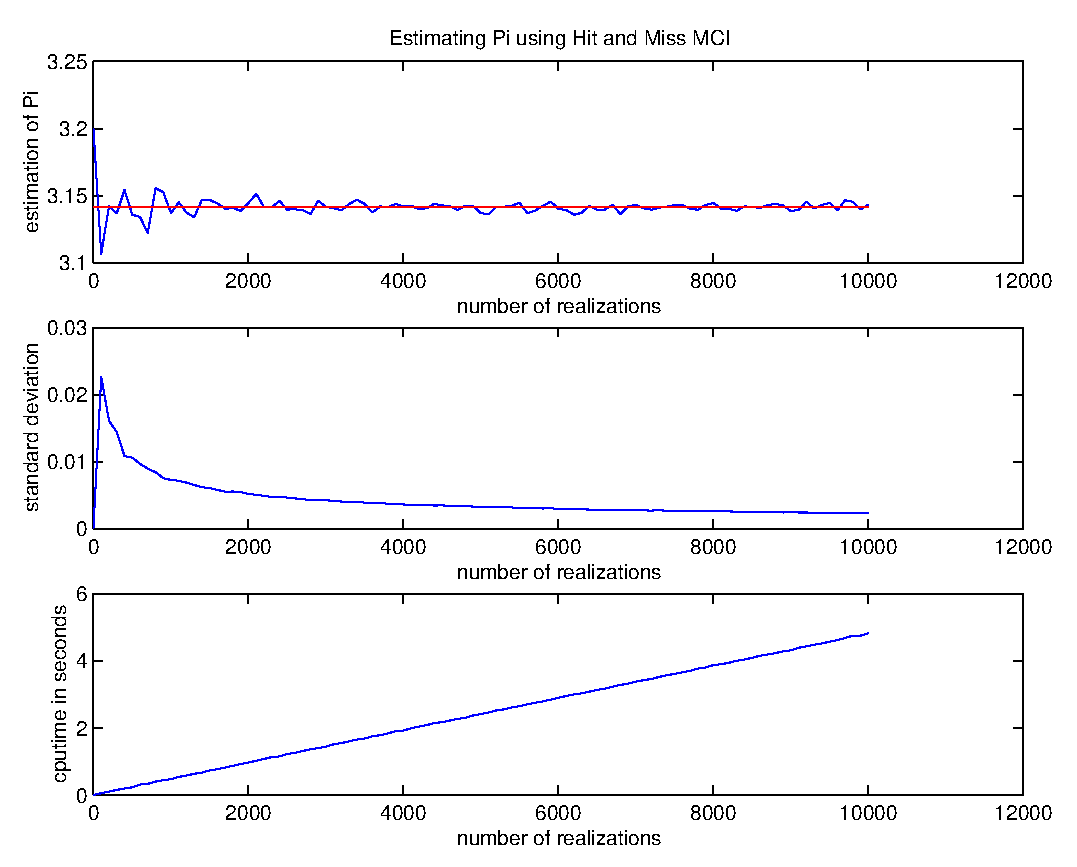
\includegraphics[width=0.44\textwidth]{f_Hit_and_Miss2_1.eps} \hfill
        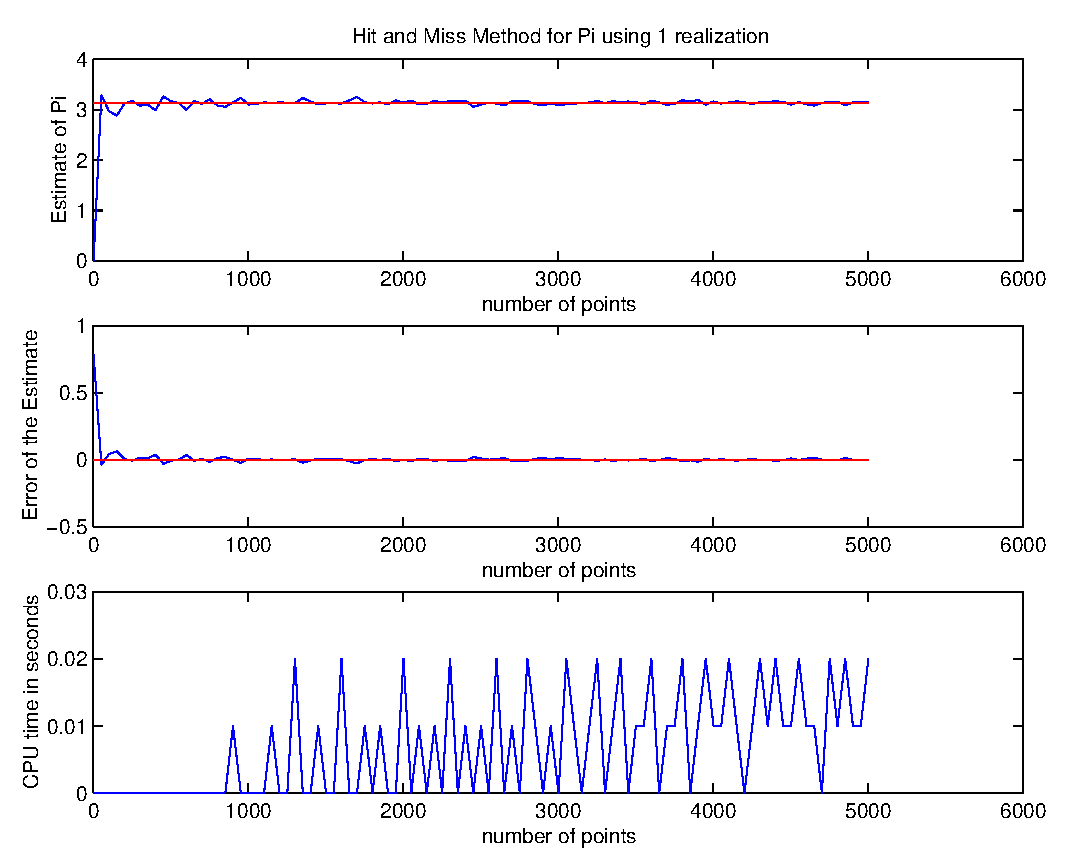
\includegraphics[width=0.44\textwidth]{f_Hit_and_Miss2_2.eps}
      \end{center}

  \item Standard Method -- \texttt{mcistandard.m}\\
    Now we use the formula $I_i=\frac{1}{n} \sum_{i=1}^n f(x_i) (b-a) $
    to estimate the integral. The mean value is
    $$ \overline{I}_i =\frac{1}{n} \sum_{i=1}^n I_i ,$$
    and the standard deviation of the individual $I_i$ is
    $$ \sigma_{I_i} = \frac{1}{N-1} \sum_{i=1}^N \left( I_i - \overline{I}
       \right)^2 = \sigma_{\overline{I}_i} \times \sqrt{n} ,$$
    where we have used the central limit theorem for the last equation to
    get the error of the mean $\sigma_{\overline{I}_i}.$

    Now we calculate several ($N$) realizations of the above algorithm
    to get a better estimate of the integral. The mean of the ensemble
    of realizations is
    $$ \overline{I}_N = \frac{1}{N} \sum_{i=1}^N \overline{I}_i . $$
    And the error of the mean is
    $$ \sigma_{\overline{I}_N} = \frac{1}{N-1} \sum_{i=1}^N \left(
      \overline{I}_i - \overline{I}_N \right)^2 =
      \sigma_{\overline{I}_i} / \sqrt{N} . $$
    Again we have used the central limit theorem and assumed that
    we have a ``representative'' $\sigma_{\overline{I}_i}$ to get
    the last equality.

    Some example outputs of the program: \\[0.5cm]
    left: Using increasing ensemble size from 1 to 5000 in steps of 100.
          Always using 50 points in the interval (a,b).\\
    right: The standard deviation and the distance to the exact result
           for the same run as in the left figure.\\
      \begin{center}
        \hspace*{-1cm}
        \includegraphics[width=0.44\textwidth]{f_MCI_Standard_3.eps} \hfill
        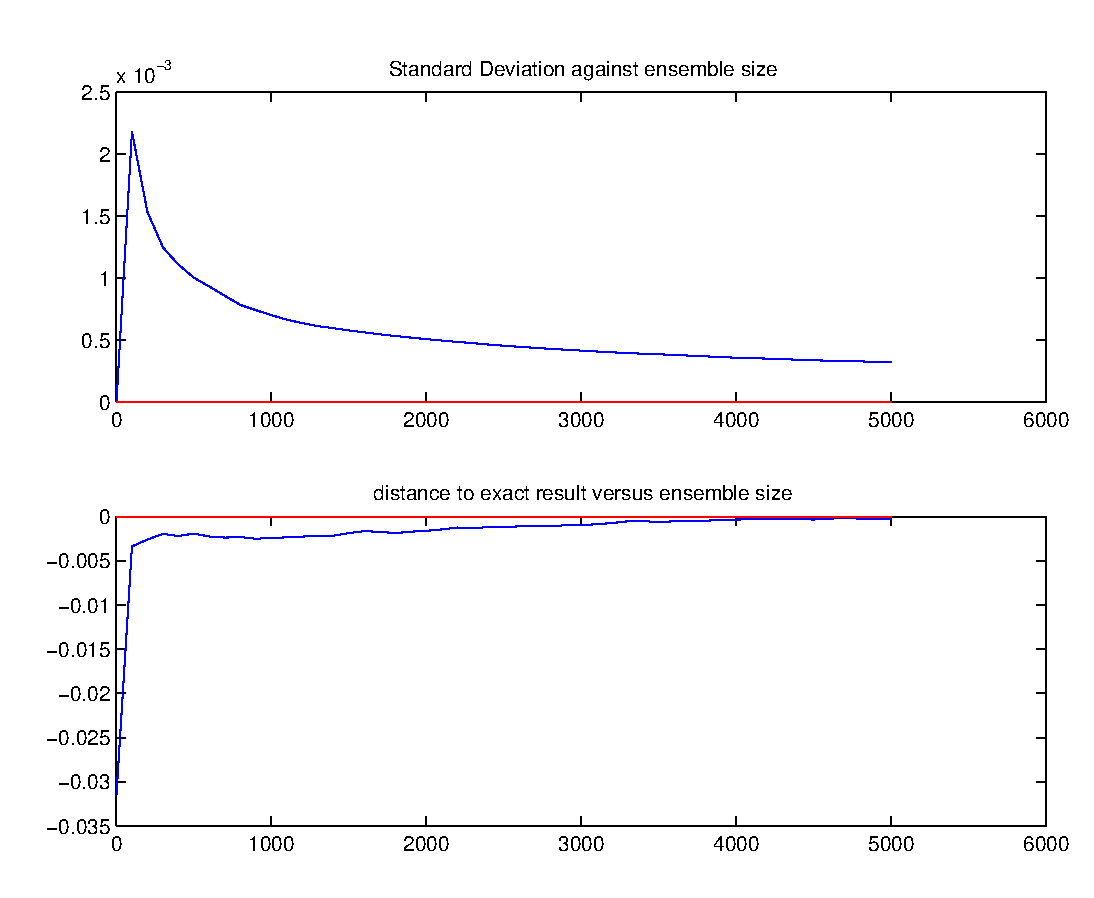
\includegraphics[width=0.44\textwidth]{f_MCI_Standard_2.eps}
      \end{center}
    The CPU time used plotted versus the accurracy of the estimate.
      \begin{center}
        \hspace*{-0.5cm}
        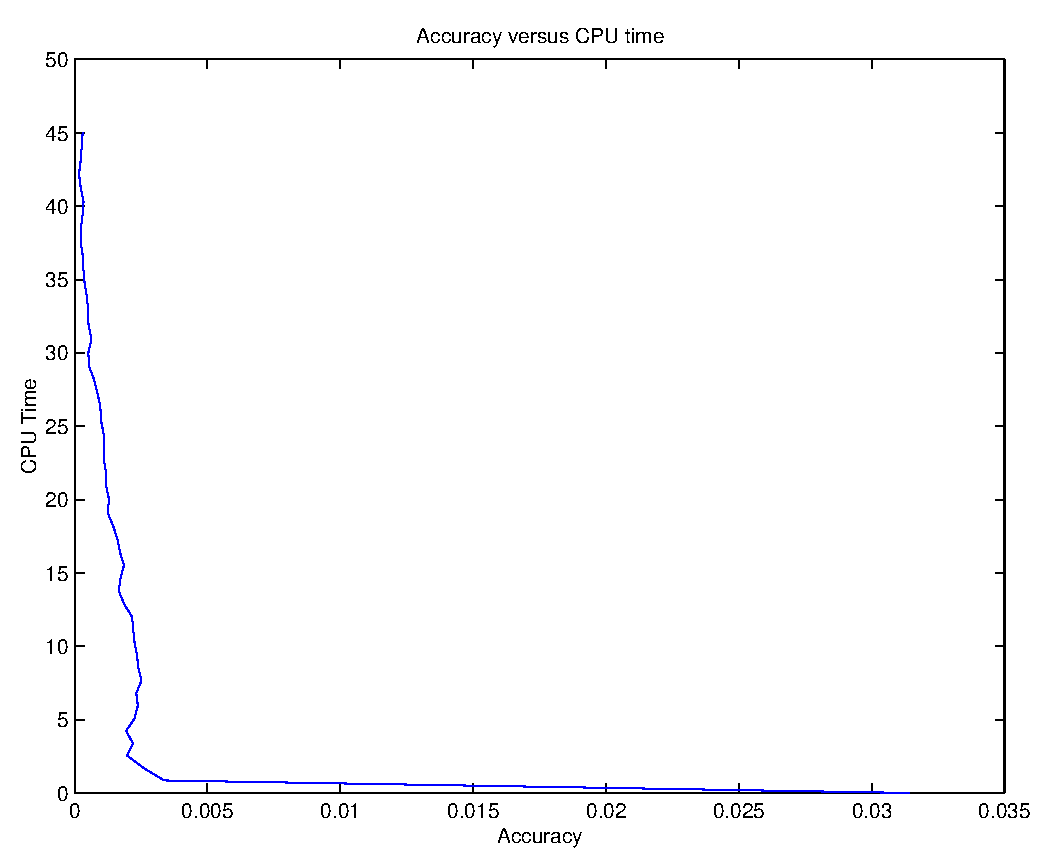
\includegraphics[width=0.5\textwidth]{f_MCI_Standard_1.eps}
      \end{center}

   \end{enumerate}
\end{Solution}

\begin{Solution}{Euler_Constant}
\textbf{Euler��s Constant using Monte-Carlo Algorithm -- \texttt{darts.m}} \\
\end{Solution}

\begin{Solution}{Standard_Deviation}
\textbf{The Standard Deviation - \texttt{variance.m} } \\
As you may soon recognize, the second and the third formula
produce by far the biggest errors, even for small samples using
very harmless distributions. But the first and the fourth method
seem to perform equally well.

For a good and extensive discussion of this problem see the good
paper by \cite[]{golub:83}. They discuss also some other algorithms
for calculating the variance. 
\end{Solution}

%%%%%%%%%%%%%%%%%%%%%%%%%%%%%%%%%%%%%%%%%%%%%%%%%%%%%%%%%%%%%%%
\section{Solutions for Chapter 2}

\begin{Solution}{Random-Number_Generator_Check}
\textbf{Random-Number Generator Check - \texttt{momentsrand.m, pokertest.m}} \\
  \begin{itemize}
  \item Moments of the \texttt{rand()} function of Matlab\\
    Example output for the first 10 moments of \texttt{rand()} using
    5000 random numbers. Shown are the mean moments of the ensemble,
    the error (standard deviation) of the mean and in the last plot
    the distribution as a histogram using 50 bins.
   \begin{center}
      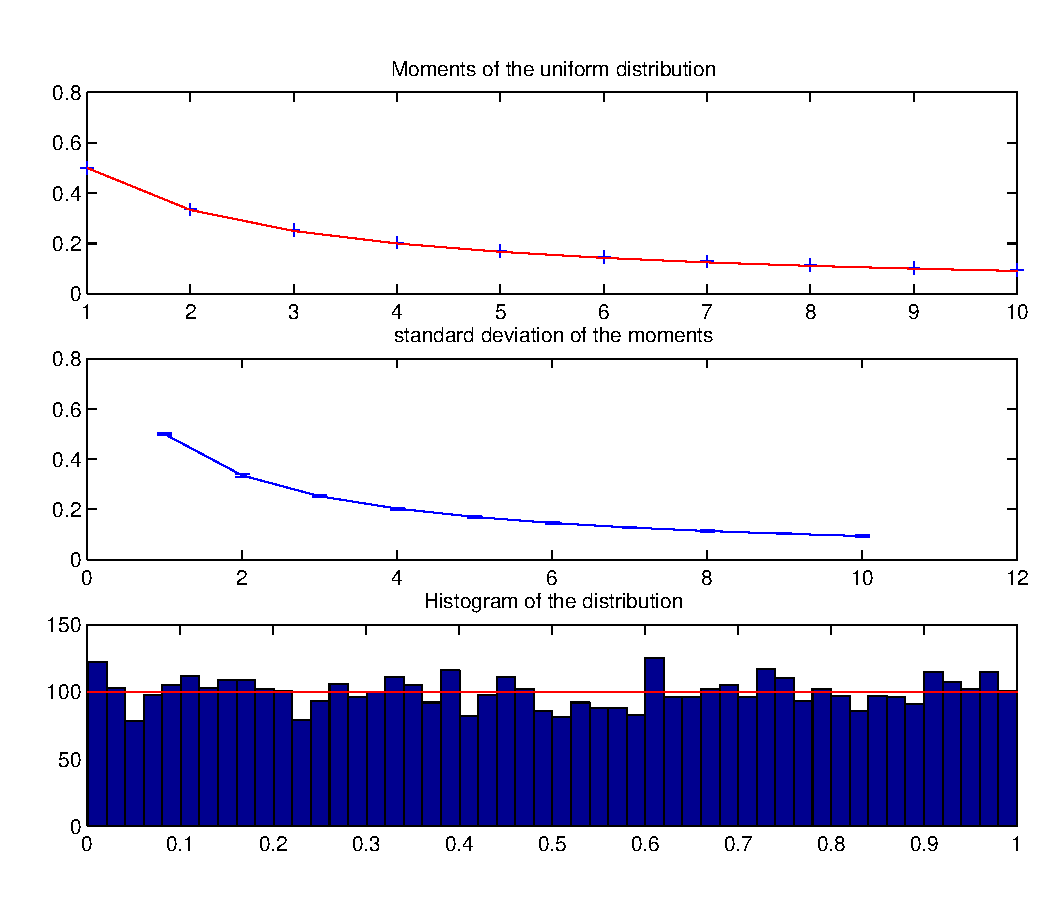
\includegraphics[width=0.8\textwidth]{f_Moments_Rand.eps}
    \end{center}
  \item Poker Test \\
    Shown are the results for a Poker test using 20000 hands, each
    using 5 random numbers (=cards). Only no pairs (=0), pairs (=1),
    three of a kind (=3) and four of a kind (=4) are counted (5 of
    a kind is obviously not allowed). The numbers above the bars are
    the actual number of hands found in the ensemble. The second plot
    shows the difference of the probability in our ensemble to the
    correct theoretical result.
    \begin{center}
      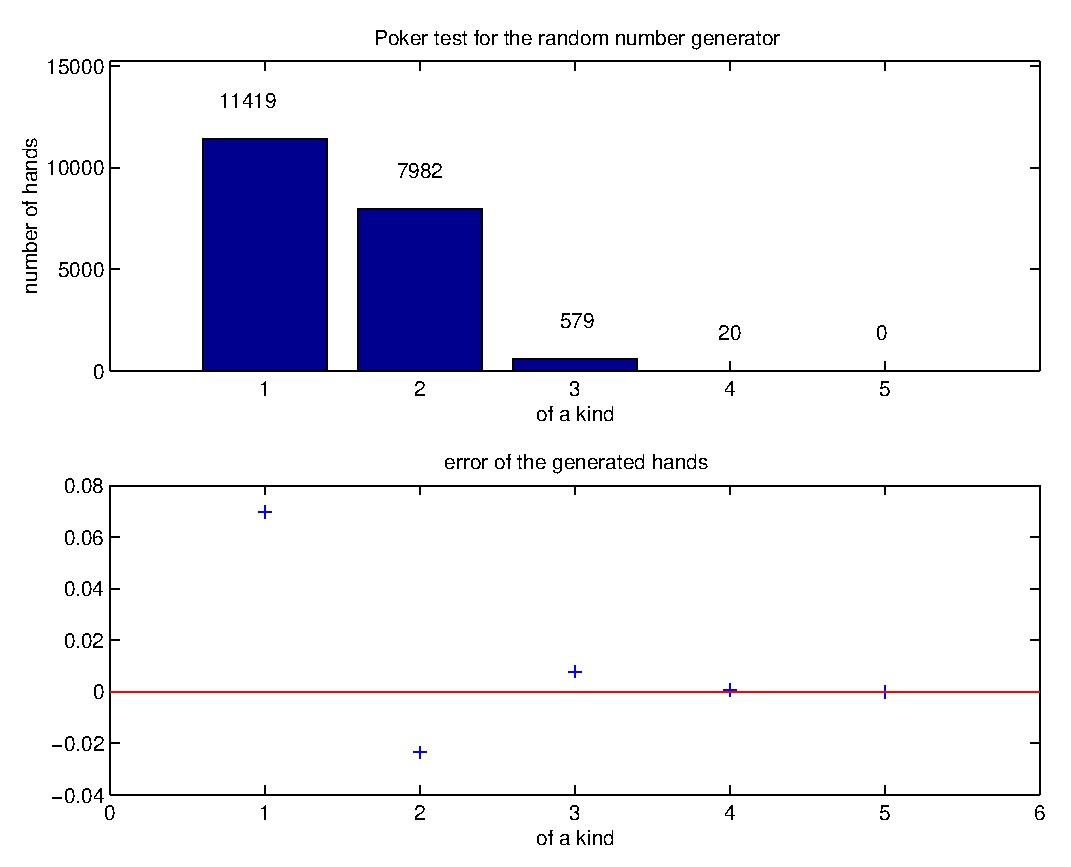
\includegraphics[width=0.8\textwidth]{f_Poker_Test.eps}
   \end{center}
 \end{itemize}   
\end{Solution}

\begin{Solution}{Galton_Board}
\textbf{Galton Board and Pascal Triangle  - \texttt{galton\_board.m}} \\
  Examples of the Galton Boards. We plot the boxes at the lower end of
  the Galton board versus the number of balls, which have fallen into
  each box. The red line indicates the normal distribution with the
  same variance and the maximum height as the ensemble generated.\\[0.5cm]
  left: using 10 rows of pins and 1000 balls \\
  right: using 20 rows of pins and 1000 balls
    \begin{center}
      \hspace*{-1cm}
      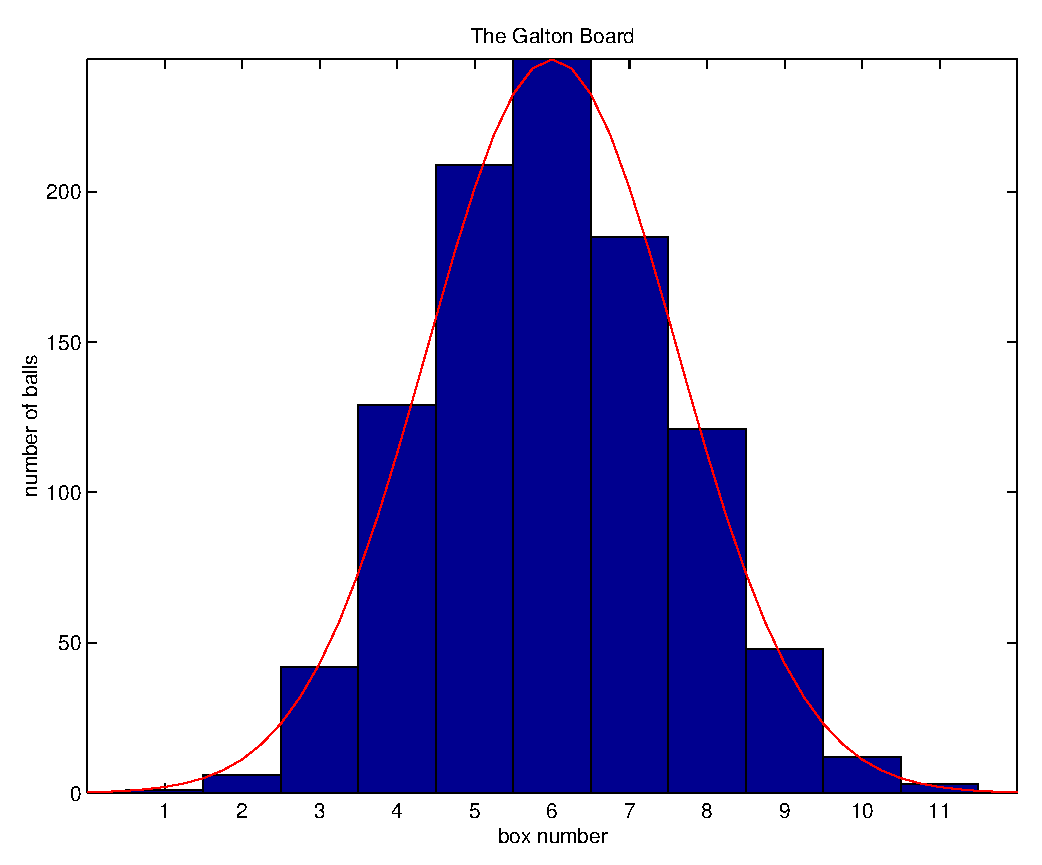
\includegraphics[width=0.45\textwidth]{f_Galton_board_3.eps}\hfill
      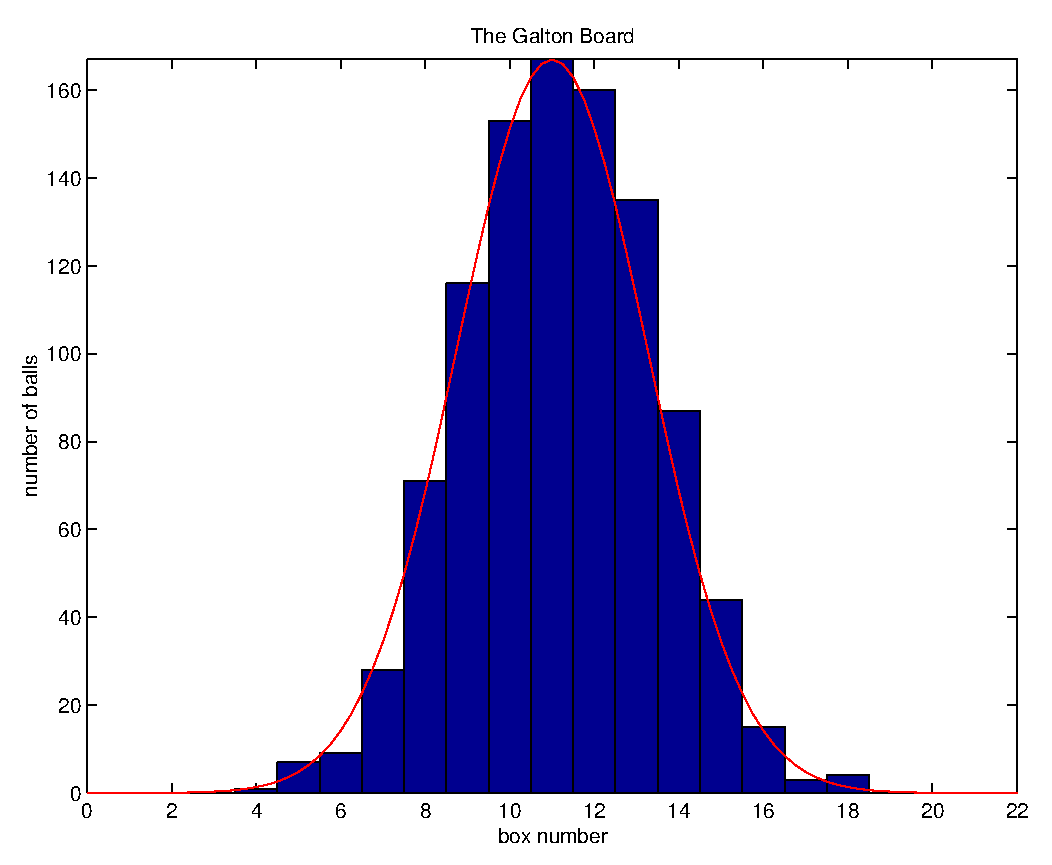
\includegraphics[width=0.45\textwidth]{f_Galton_board_1.eps}
   \end{center}

   using 200 rows and 16000 balls
    \begin{center}
      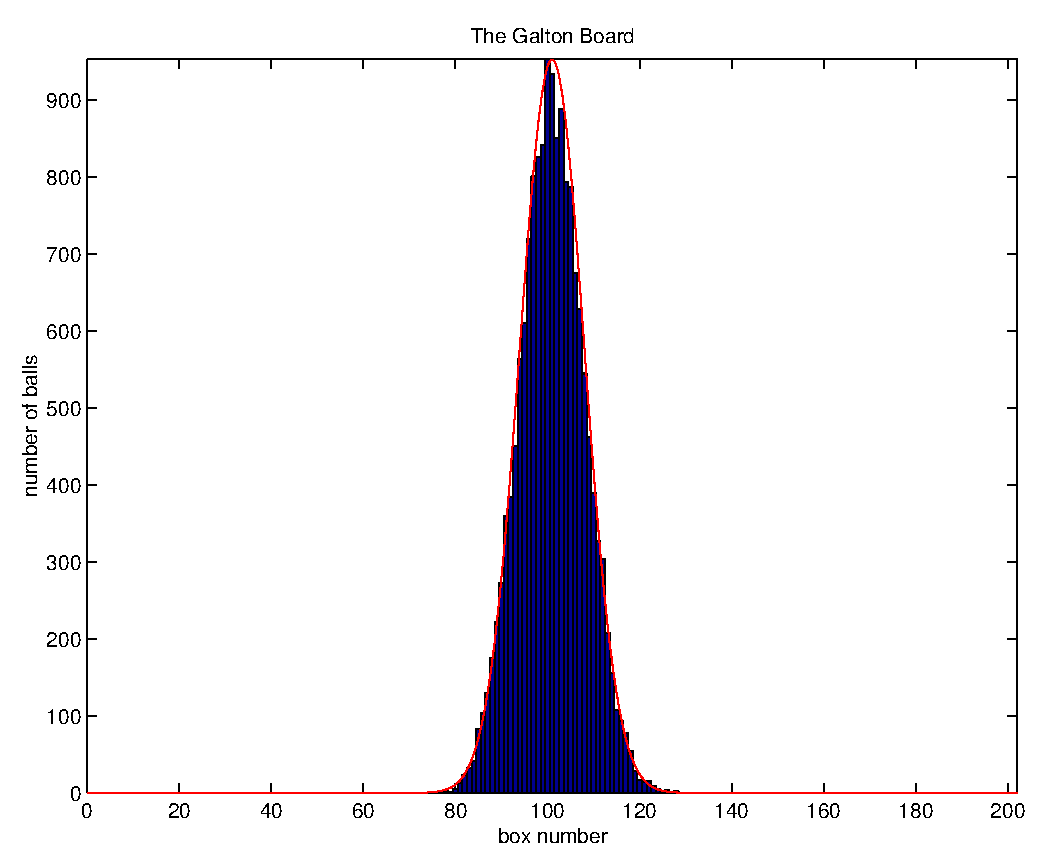
\includegraphics[width=0.8\textwidth]{f_Galton_board_2.eps}
   \end{center}

   The connection to the Pascal trinagle is obvious, if you know how to
   get the number of balls in the next row (say n+1) from the number of
   balls in the boxes of the previous row (say n). That��s exactly like
   in the Pascal triangle:
   \begin{center}
     1 \\
     1 1 \\
     1 2 1 \\
     1 3 3 1 \\
     1 4 6 4 1 \\
     1 5 10 10 5 1 \\
     1 6 15 20 15 6 1
   \end{center}
   You start with row 2 of the Pascal triangle, which corresponds to
   one pin (1 row) in the Galton board. The sum in each row is $2^N$ in
   row $N$. Therefore the probability for each box of a row of the
   Galton board is just the corresponding number of the Pascal triangle
   divided by $2^N.$          
\end{Solution}

%%%%%%%%%%%%%%%%%%%%%%%%%%%%%%%%%%%%%%%%%%%%%%%%%%%%%%%%%%%%%%%
\section{Solutions for Chapter 3}

\begin{Solution}{Random-Number_Generator}
\textbf{Random-Number Generator - \texttt{linear\_con.m} } \\
    All plots use the linear congruential method with the parameters
    given in the assignment. The input parameters are: Initial seed $1$
    and 1000 random numbers are generated.

    The first plots show the generated random numbers, the second ones
    show the histogram of the distribution. The third ones show 2D vectors
    and the fourth ones 3D vectors from the generated sequence of random
    numbers.
    \begin{itemize}
    \item parameter set 1 \\
      \begin{center}
        \hspace*{-1cm}
        \includegraphics[width=0.47\textwidth]{f_linear_con1a.eps}\hfill
        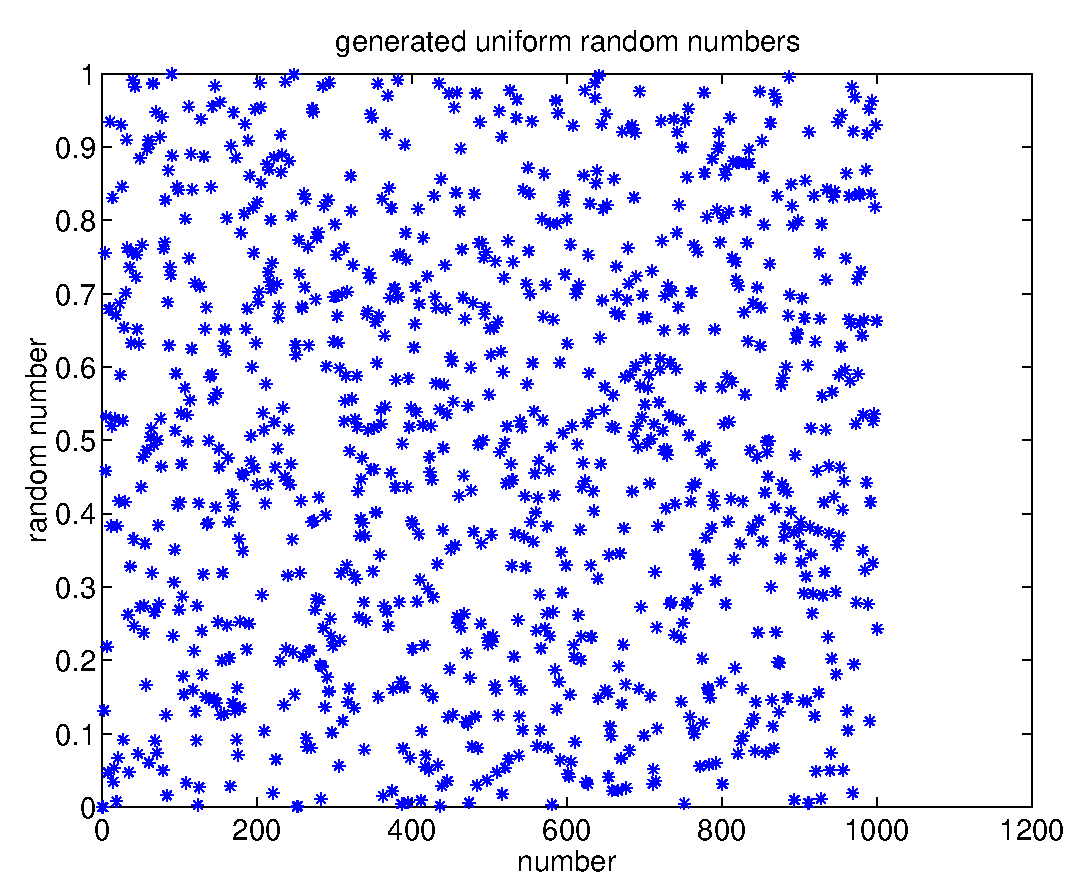
\includegraphics[width=0.47\textwidth]{f_linear_con1b.eps}
      \end{center}
      \begin{center}
        \hspace*{-1cm}
        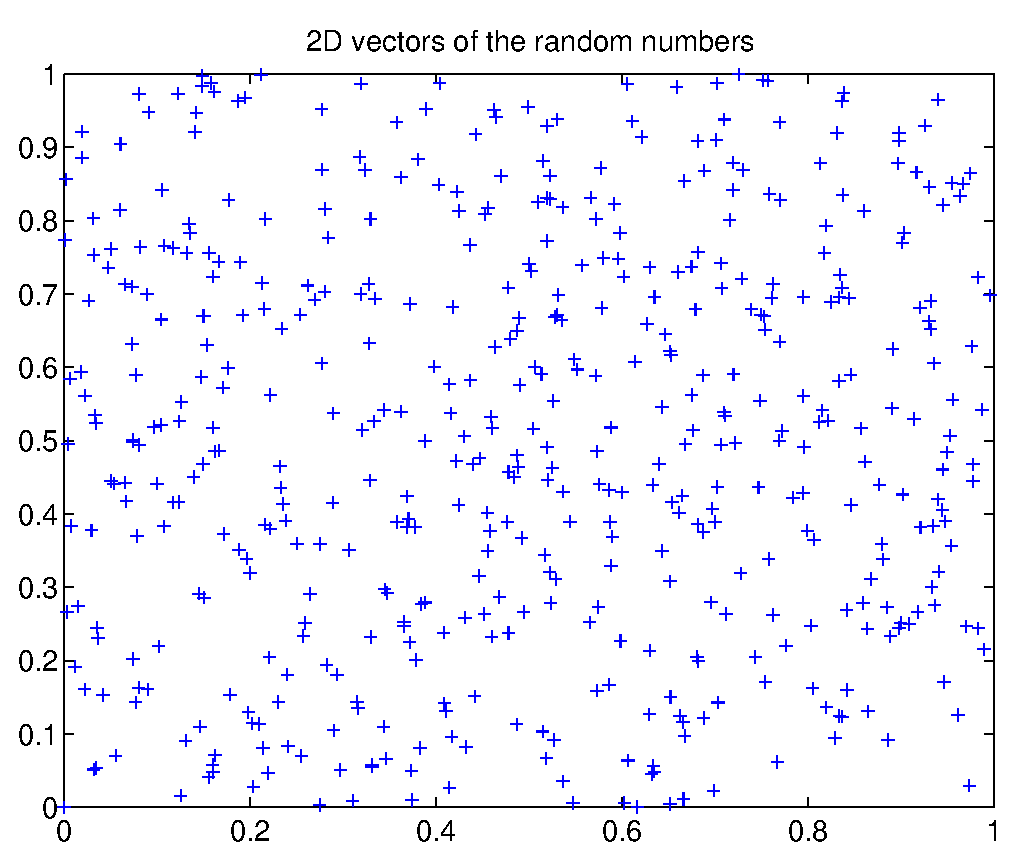
\includegraphics[width=0.47\textwidth]{f_linear_con1c.eps}\hfill
        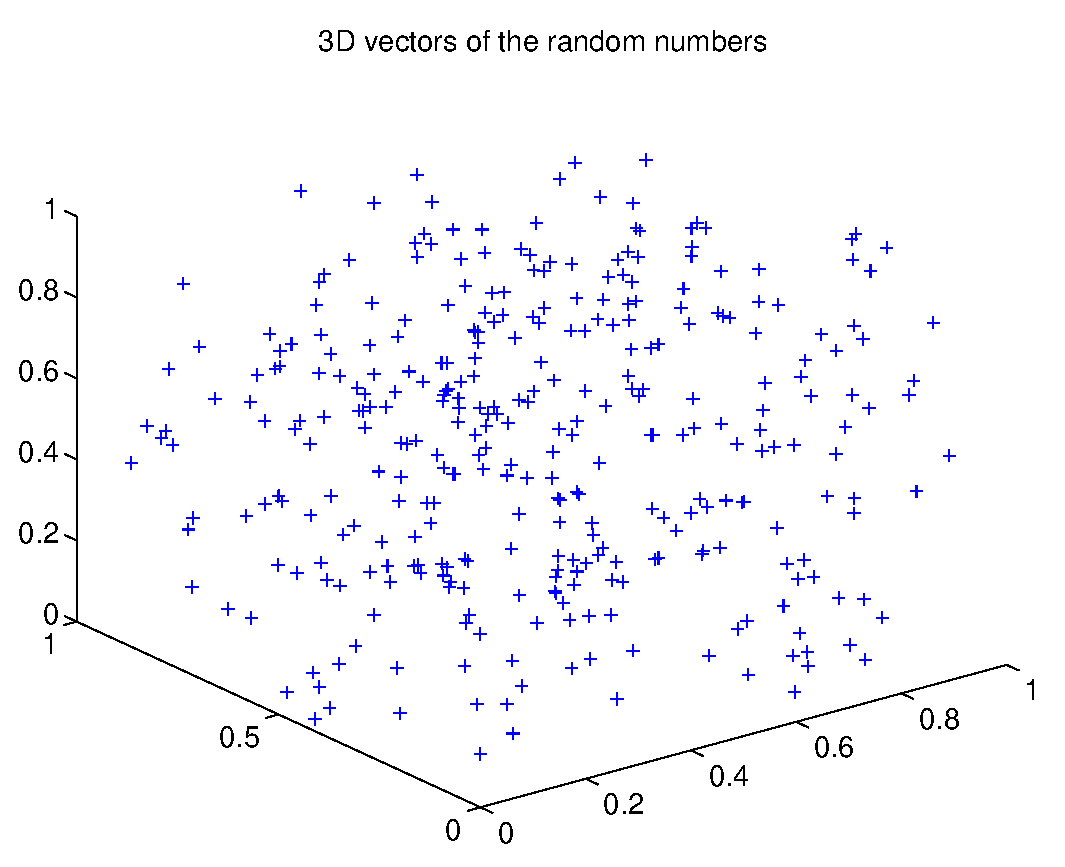
\includegraphics[width=0.47\textwidth]{f_linear_con1d.eps}
      \end{center}
    \item parameter set 2 \\
      \begin{center}
        \hspace*{-1cm}
        \includegraphics[width=0.47\textwidth]{f_linear_con2a.eps}\hfill
        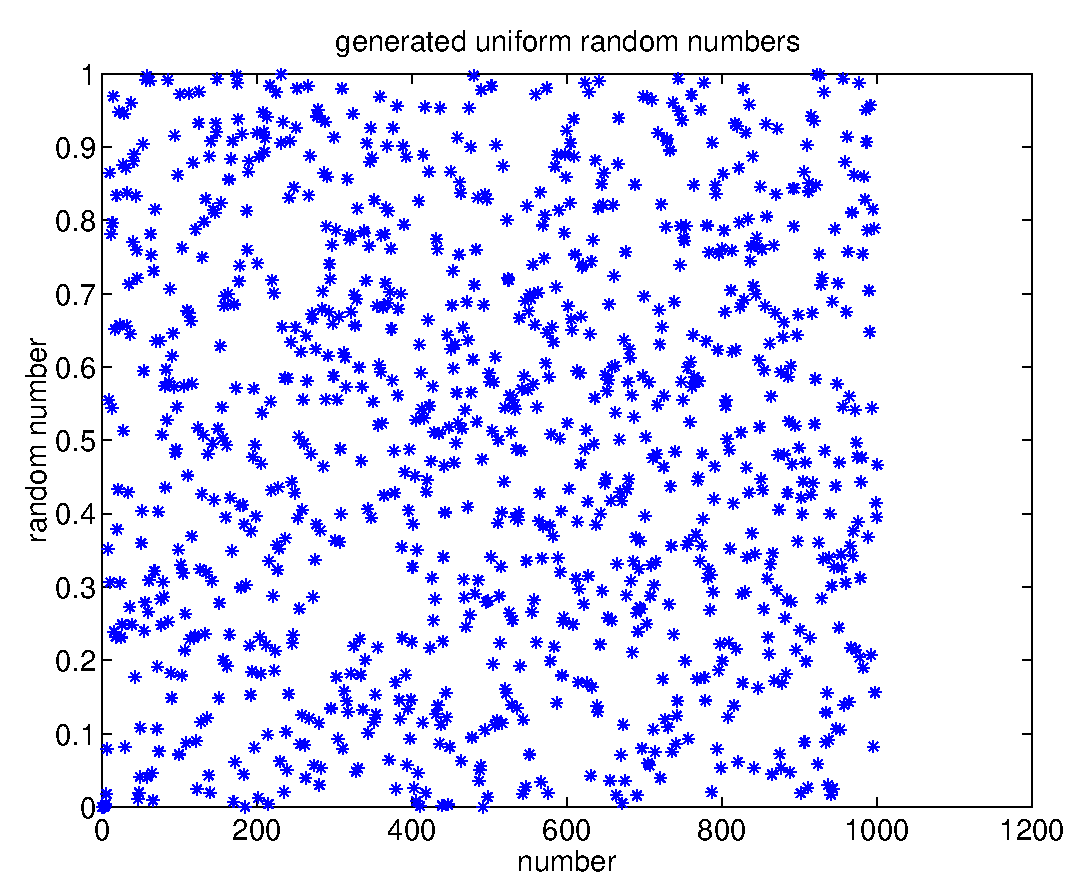
\includegraphics[width=0.47\textwidth]{f_linear_con2b.eps}
      \end{center}
      \begin{center}
        \hspace*{-1cm}
        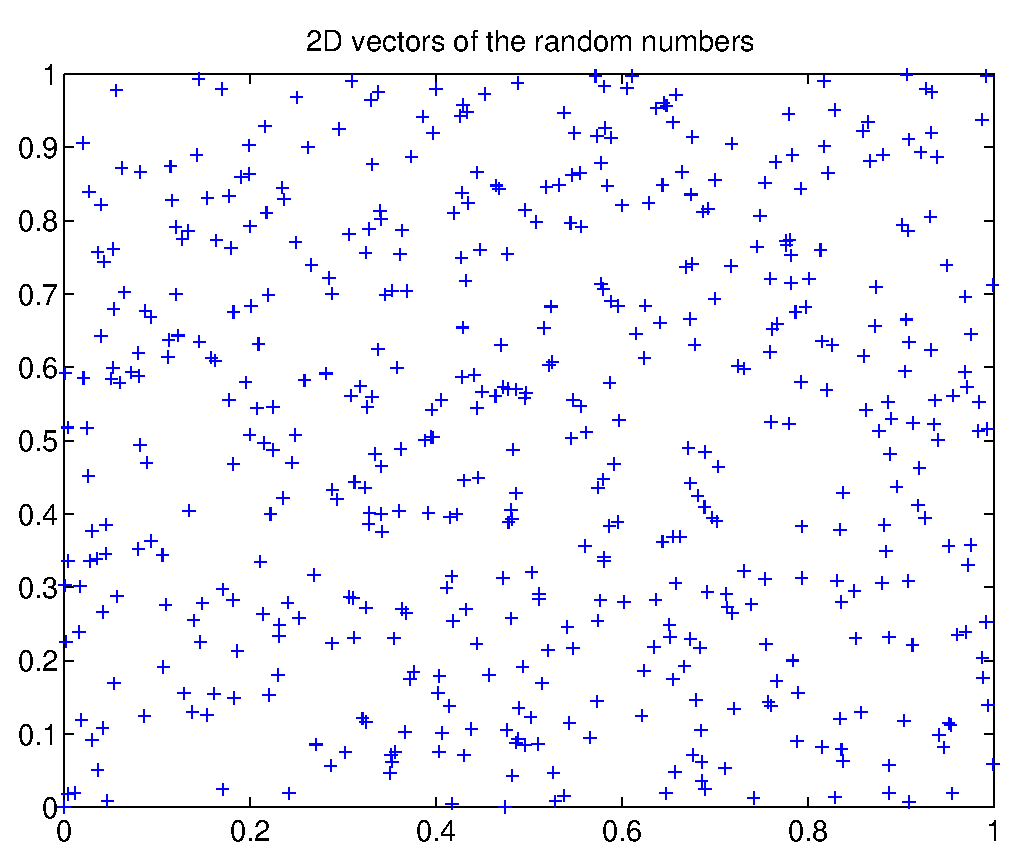
\includegraphics[width=0.47\textwidth]{f_linear_con2c.eps}\hfill
        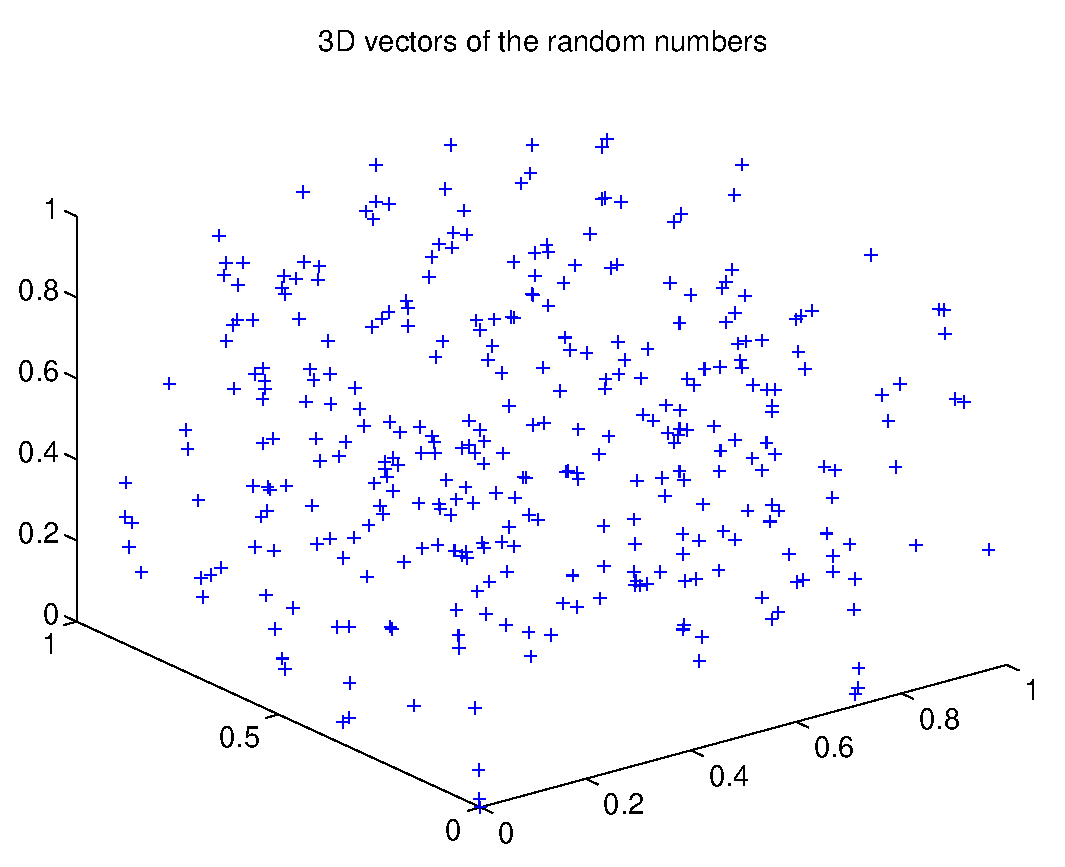
\includegraphics[width=0.47\textwidth]{f_linear_con2d.eps}
      \end{center}
    \end{itemize} 

    At first you don��t see any difference between the two and you
    don��t think of any problems. But if you plot the 3D vectors and
    use the \texttt{rotate3d} command with Matlab to rotate the
    3D plot, you can see plots like the ones below. On the left the
    plot is rotated until you see the planes and on the right you wouldn��t
    expect correlations. Both plots use the same sample of 5000 random numbers.
    This clearly
    visualizes the correlation between successive triple random numbers.
    \begin{center}
      \hspace*{-1cm}
      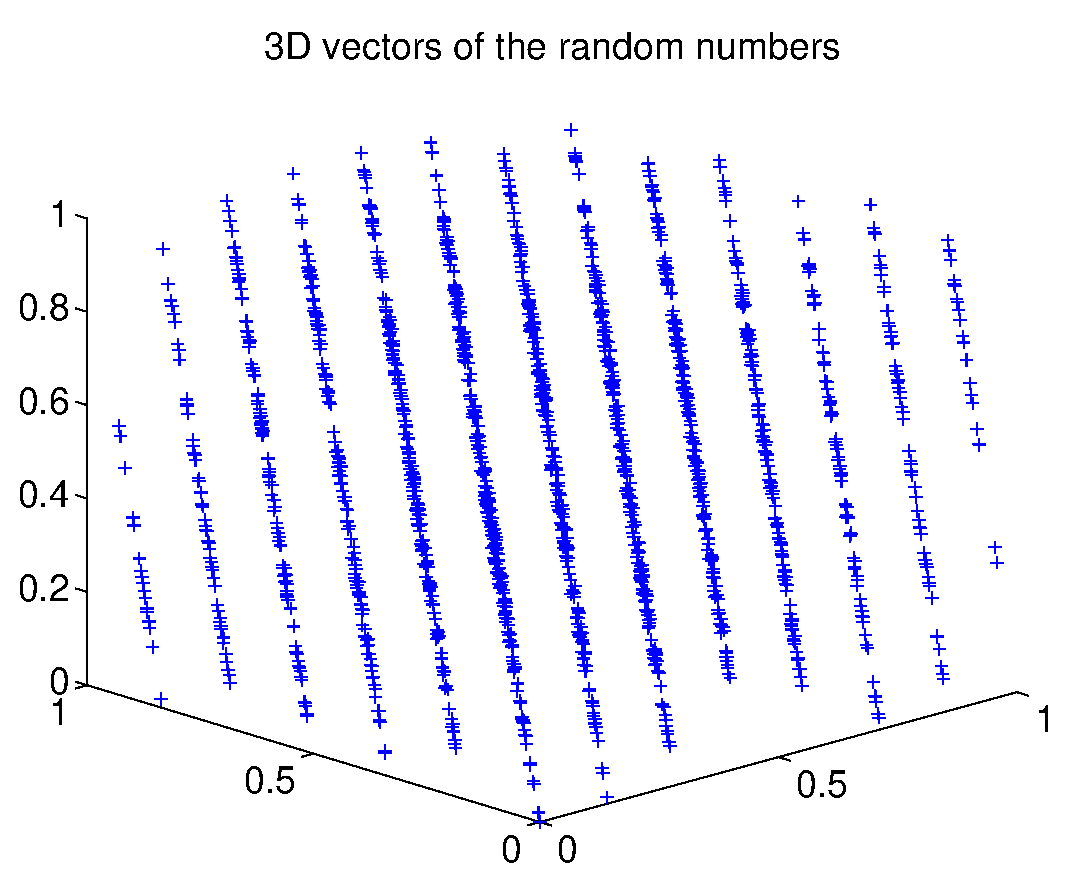
\includegraphics[width=0.47\textwidth]{f_linear_con_3d_1.eps}\hfill
      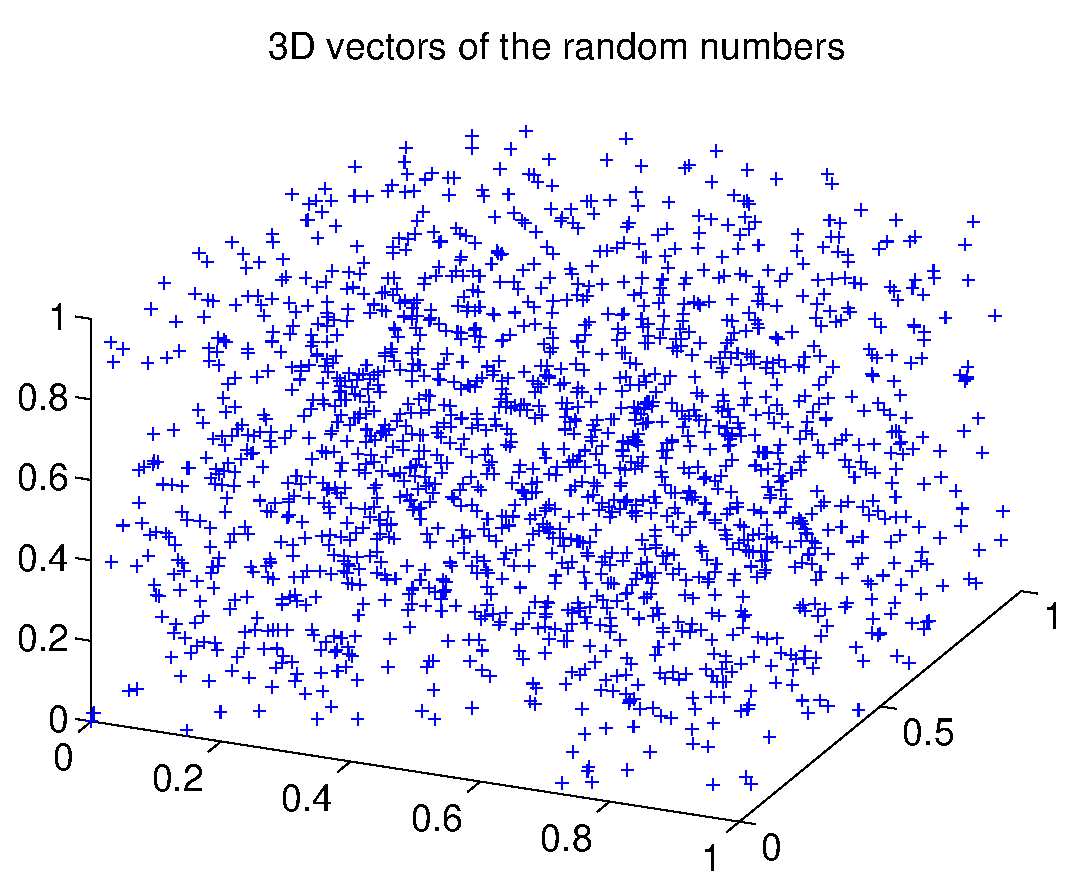
\includegraphics[width=0.47\textwidth]{f_linear_con_3d_2.eps}
    \end{center}
\end{Solution}

\begin{Solution}{Poisson_Distribution}
\textbf{Poisson distribution - \texttt{poisson.m}} \\
  The first figure shows the generated Poisson distributed random
  numbers. The second figure shows two dimensional vectors of Poisson
  distributed random numbers. The last (third) figure finally shows
  the histogram of the generated sequence and the exact Poisson
  distribution.

  The parameters for this run have been:
  $$\lambda = 10 \quad \text{and}\quad N=1000 \quad .$$

  \begin{center}
    \hspace*{-1cm}
    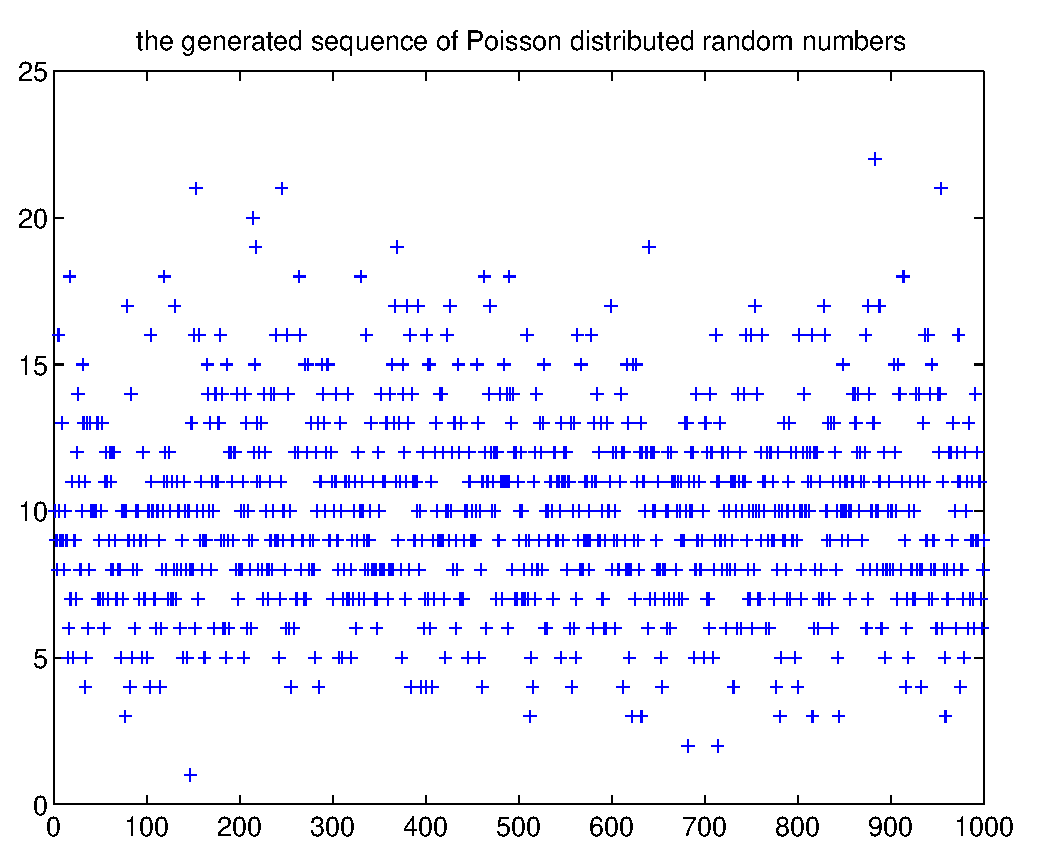
\includegraphics[width=0.47\textwidth]{f_poisson_1.eps}\hfill
    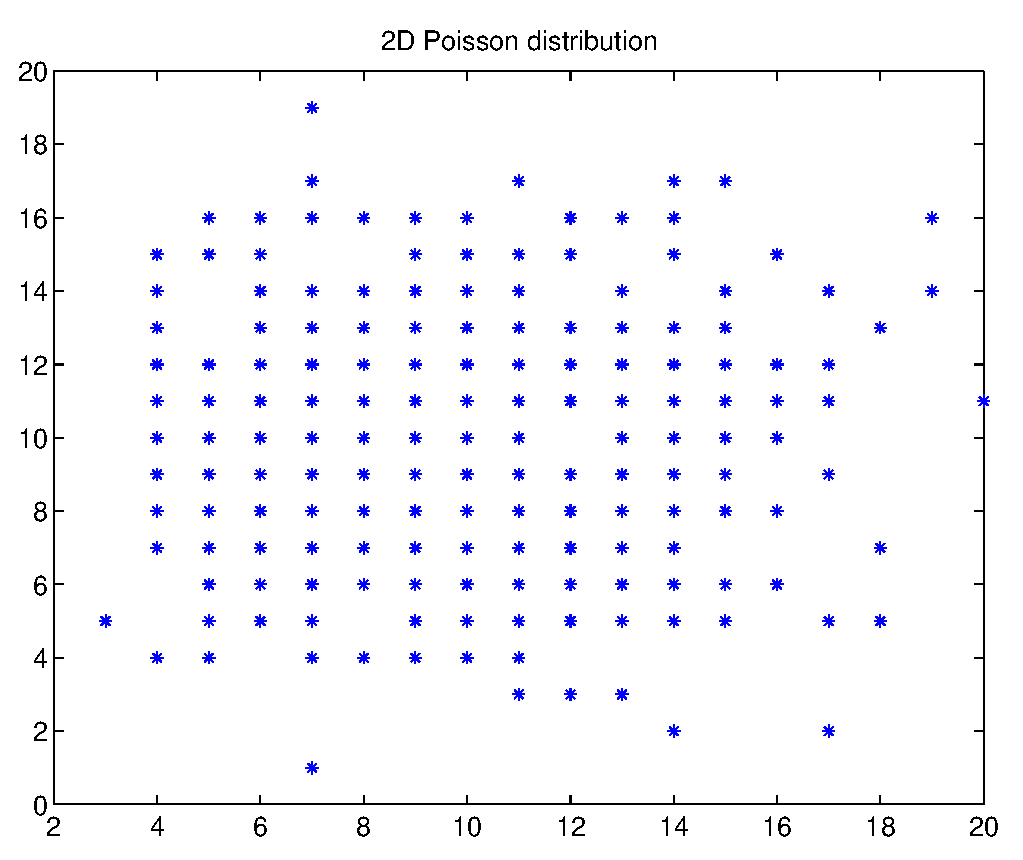
\includegraphics[width=0.47\textwidth]{f_poisson_3.eps}
  \end{center}
  \begin{center}
    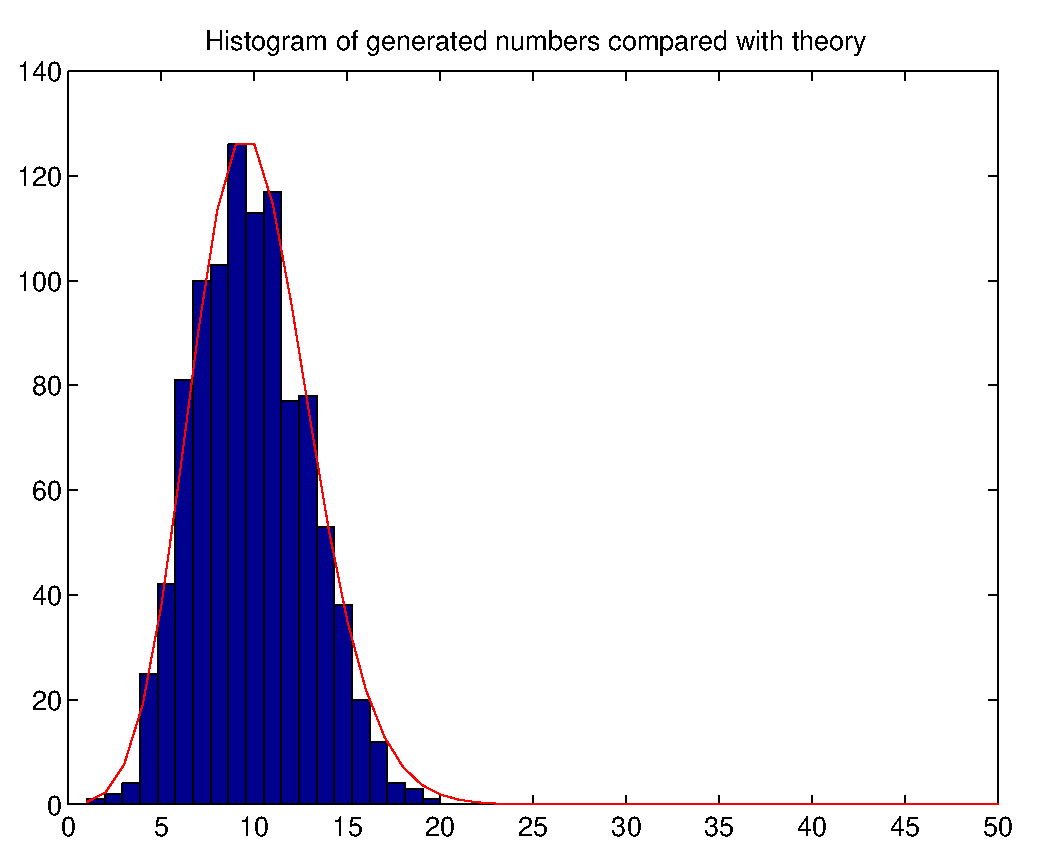
\includegraphics[width=0.8\textwidth]{f_poisson_2.eps}\hfill
  \end{center}

  Just a few comments about the method used.
  Often the Poisson distribution is written as
  $$ P_{\lambda t} (n)= e^{-\lambda t} \frac{\left(\lambda t\right)^n}{n!} ,$$
  with the parameter $\lambda t$. We have chosen $t$ to be one and so
  referring to a unit interval of time. In that sense $\lambda$ is the
  average number of events per unit time (and as you already know, it is
  actually the mean of the Poisson distribution).

  Now, the algorithm used is
  based on the fact that if the time intervals $T_i$ between events
  are from $\exp(-\lambda T_i)$, then the number of events occurring
  in an unit interval of time is from $P_\lambda(n)$ (Poisson distributed).

  To proof that, you need the theorem: if $X_1,\ldots ,X_n$ are mutually
  independent random variables with the exponential density
  $$p(x)=\lambda e^{-\lambda x}$$
  then the sum $S_N:=X_1+\cdots+X_n$ has a density
  $$ g_n(x) = \lambda \frac{(\lambda x)^{n-1}}{(n-1)!} e^{-\lambda x} .$$
  (This is a so called gamma density.) The proof can be done by
  induction. For the exponential distribution
  function $F(x)=1-e^{-\lambda x}$ we get the distribution function of $S_N$ as
  $$ G_n(x) = 1- e^{-\lambda x} \left( 1+\frac{\lambda x}{1!} + \cdots
    \frac{(\lambda x)^{n-1}}{(n-1)!} \right) .$$

  The second step is to introduce a new family of random variables
  $N(t)$: $N(t)$ is the number of indices $k\geq 1$ such that $S_k\leq t.$
  ($S_k$ is the sum opf exponentially distributed r.v. from above.)
  Because $S_n$ has the distribution $G_n(x)$ (see theorem above),
  the probability of events $\{N(t)=n\}$ has the distribution
  $$ P(\{N(t)=n\}= G_n(t)-G_{n+1}(t) = e^{-\lambda t} \frac{(\lambda t)^n}{n!}.$$
  That is exactly a Poisson distribution!

  For details see \cite[page 8-12]{feller2:71}.
\end{Solution}
\begin{Solution}{Acceptance-Rejection-Method}
\textbf{Acceptance-Rejection-Method - \texttt{rejection.m} } \\
  First of all we have to note that the volume of the n-dimensional
  sphere is given by
  $$ V_{R,n} = R^n \times V_{1,n} = R^n \times \frac{\pi^{n/2}}{\Gamma(n/2+1)},$$
  where $\Gamma(x)$ is the well known Gamma function:
  $$\Gamma(x):= \int_0^\infty e^{-t} t^{x-1} dt = \lim_{n\to\infty} n^x
    \frac{(n-1)!}{x(x+1)(x+2) \cdots (x+n-1)} \quad \text{for x >0}.$$
  (for all real numbers, except $0, -1, -2 \ldots.$
  We have $\Gamma(x+1)=x\Gamma(x)$ and therefore for natural numbers $n>0$
  $\Gamma(n+1)=n!.$ As you can see in the figure, the volume of the sphere
  (red diamonds/line)
  is decreasing by going to higher dimensions (keeping the radius $R=1$ constant).
  \begin{center}
    \hspace*{-1cm}
    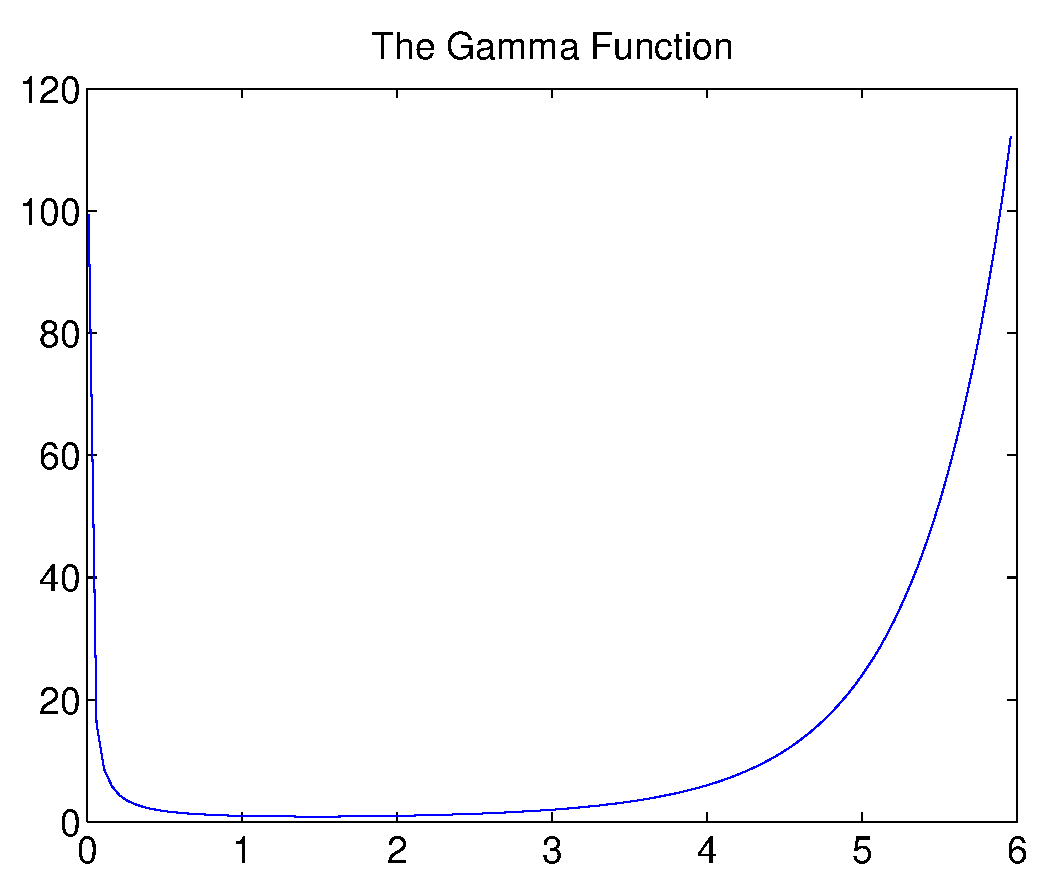
\includegraphics[width=0.47\textwidth]{f_gamma.eps}\hfill
    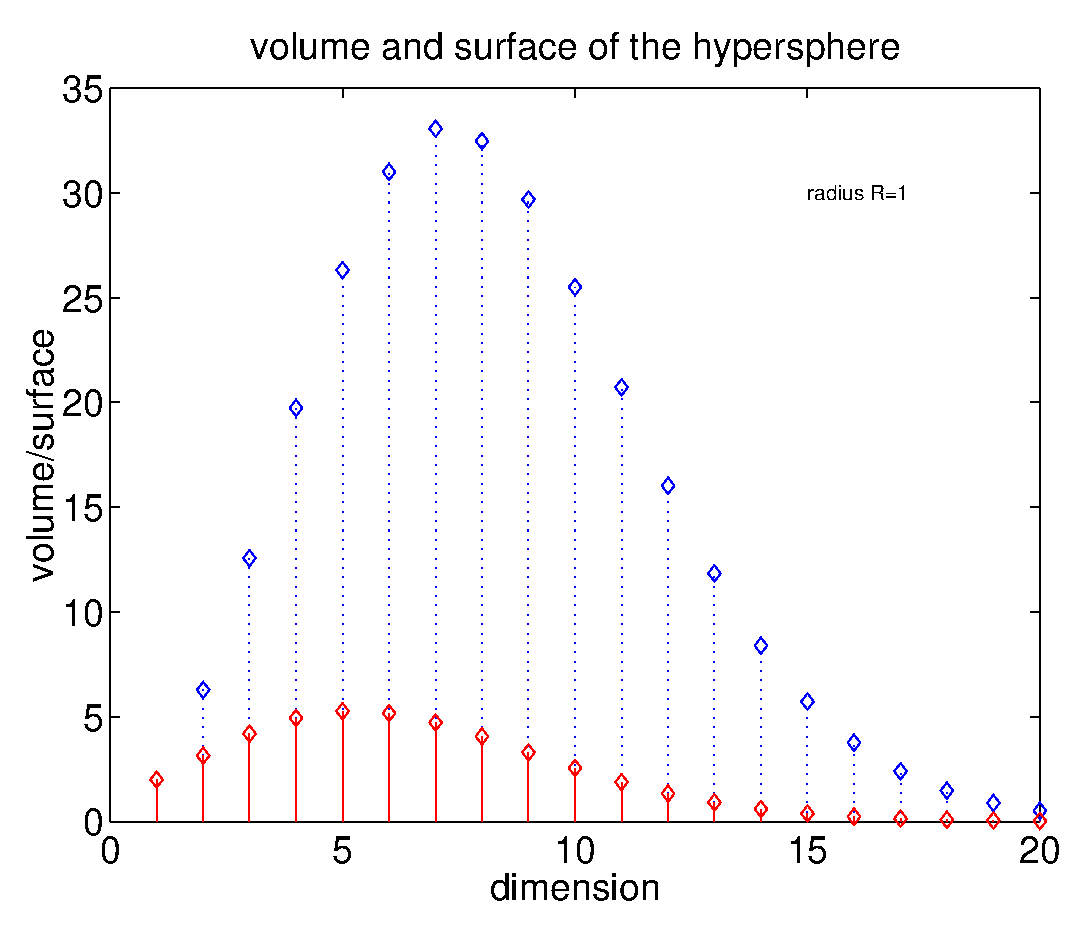
\includegraphics[width=0.47\textwidth]{f_sphere.eps}
  \end{center}

  You get the surface of the sphere by just differentiating the formula above
  and get (see blue diamonds/line)
  $$ S_{R,n} = \frac{d}{dR} V_{R,n} =
  n R^{n-1} \times \frac{\pi^{n/2}}{\Gamma(n/2+1)}.$$
  \begin{center}
    \hspace*{-1cm}
    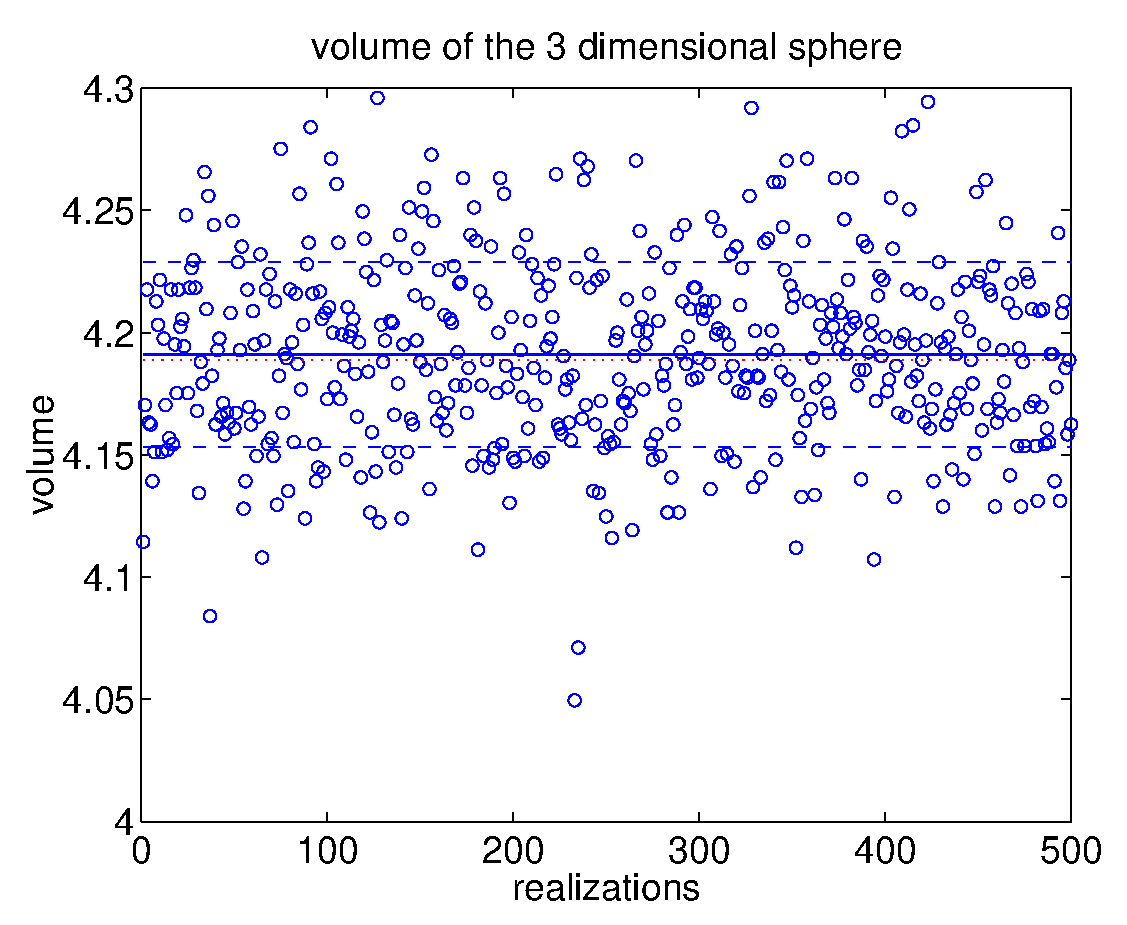
\includegraphics[width=0.47\textwidth]{f_rejection_1.eps}\hfill
    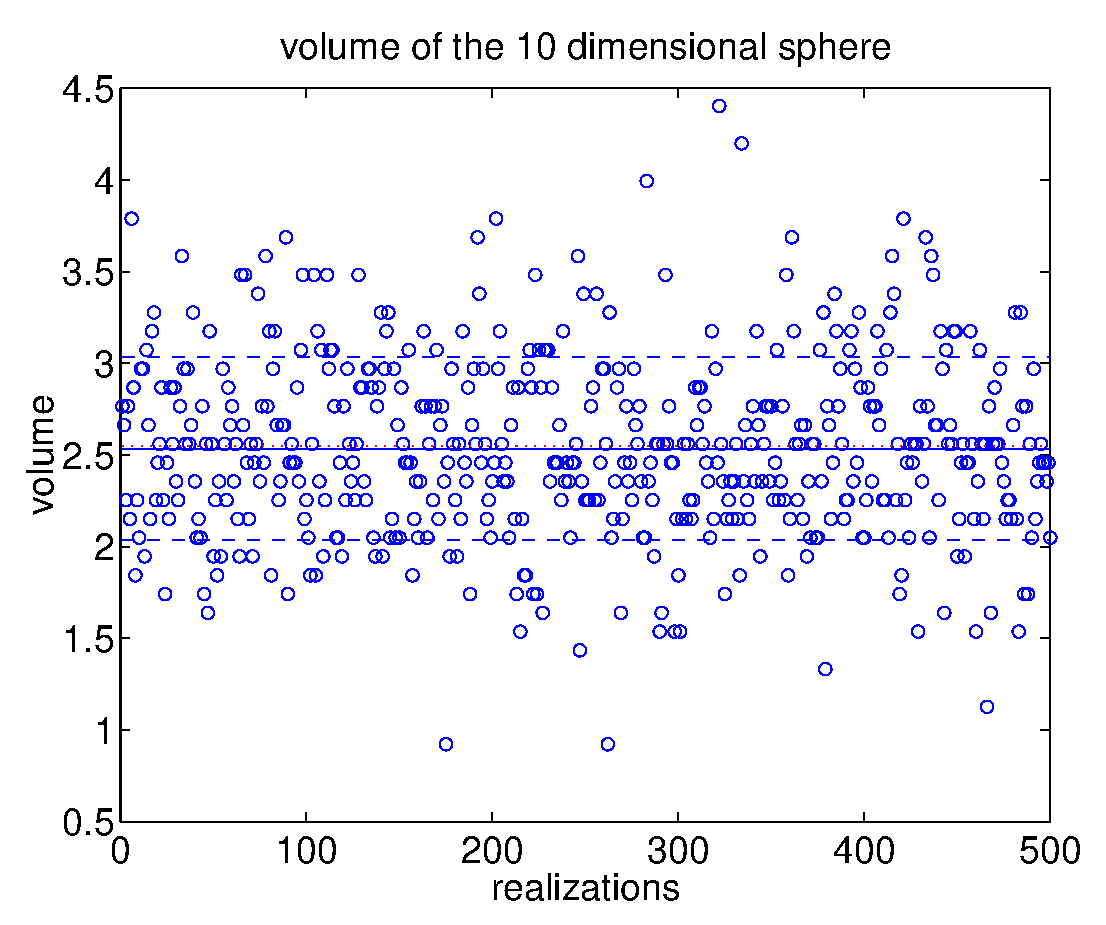
\includegraphics[width=0.47\textwidth]{f_rejection_2.eps}
  \end{center}
  The blue lines represent the sample mean and the sample variance and
  the red line is the exact value.
  Both figures are made using 500 realizations each drawing 10000 points
  in the n-dimensional space. The result for the left figure was
  $V=4,1910\pm0,0017$ (exact $V=4,1888$), for the right figure we got
  $V=2,534\pm0,022$ (exact $V=2,550$).

  The algorithm for the surface of the hyper sphere is exactly the same,
  except that in the case of an accepted hit, you have to divide the
  accepted coordinates by the radius $R$. This gives you a point on the
  surface of the sphere.
  \begin{center}
    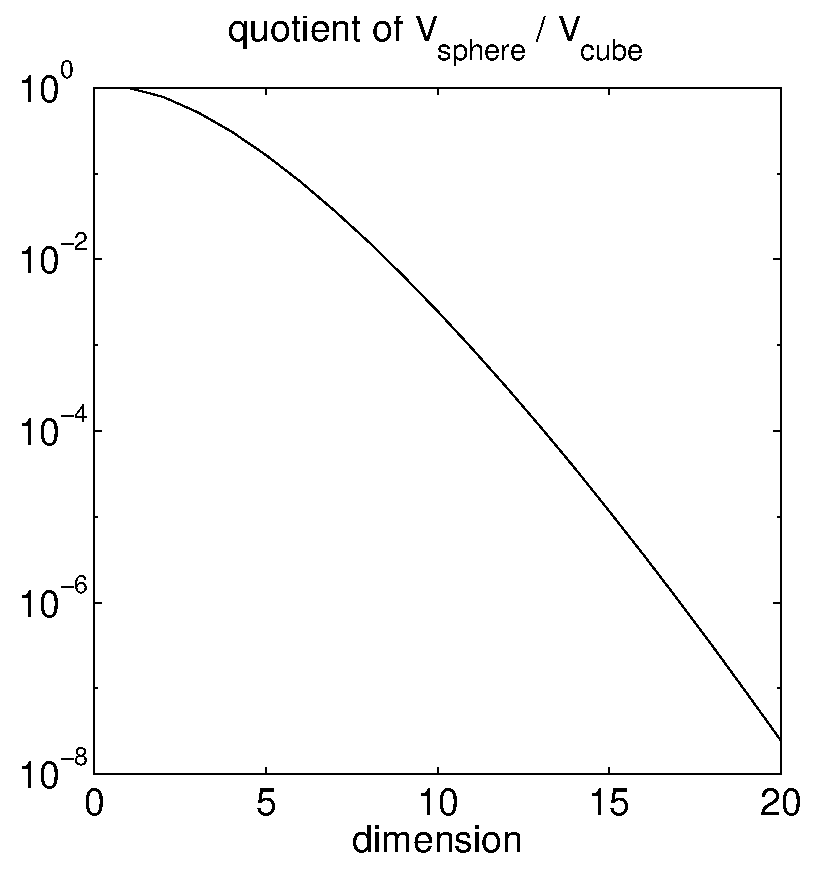
\includegraphics[width=0.47\textwidth]{f_rejection_efficiency.eps}
  \end{center}
  As you can see from the plots above, the method is getting worse with
  increasing dimension, because $V_{\text{hypersphere}}/V_{\text{hypercube}}$
  is going to zero for large $n$.
\end{Solution}

\begin{Solution}{Importance_Sampling}
\textbf{Importance Sampling - \texttt{importance.m}} \\
  The idea of the importance sampling here is instead of sampling
  uniform random numbers and putting it into the function, we
  use normally distributed random numbers.

  {\bf A very good book about importance sampling is
  \cite[Chapter 3 and 4.1]{kalos:86}.}

  \begin{itemize}
  \item Standard sampling:\\
    $$ I_S= \frac{c}{N} \sum_{i=1}^N f(\xi) ,$$
    where the $\xi$ are from a uniform distribution.\\
    Easy to implement and understand, but the error is usually very
    big.
  \item Importance sampling:\\
    Here we suggested to use a normal distribution instead of the
    uniform one for the $\xi$. Then the formula reduces to:
    $$ I_I = \frac{1}{N} \sum_{i=1}^N |\xi| \times
       \frac{\sqrt{2 \pi \sigma^2}}{2} \times \frac{1}{\sqrt{2}} =
       \frac{\sqrt{\pi}}{2 N} \sum_{i=1}^N |\xi| .$$
    First of all you have to realize that the \texttt{randn()} function
    of Matlab produces normally distr. random numbers with mean $\mu=0$
    and variance $\sigma^2=1$. It also produces random numbers in the
    open interval $(-\infty,+\infty)$ and not, like desired, in the
    interval $[0,+\infty).$

    To correct for that, use the fact, that
    $$ \int_0^\infty ve^{-v^2}dv = \frac{1}{2} \int_{-\infty}^{+\infty}
      |v| e^{-v^2}.$$
    (because the function is symmetric with respect to the y-axis.)
    Matlab produces numbers from
    $$ p(x)=\frac{1}{\sqrt{2\pi\sigma^2}}
                \exp(-\frac{(x-\mu)^2}{2\sigma^2}), \mu=0, \sigma^2=1.$$
    Now we have to transform this density to one with variance
    $\sigma^2=1/2,$ which then has the form appearing in our integral
    $(e^{-v^2}).$ We just divide the random number generated
    with \texttt{randn()} by $\sqrt{2}.$

    Then we accept only random numbers falling in the interval $[-c,c],$
    because we are integrating over that interval (we have to take this into
    account, when calulating moments). Actually we do not    
    need that restriction, but it demonstrates some additional complications, which
    could arise in actual problems.

    The last step is to correct for the additional factor
    $\sqrt{2 \pi \sigma^2}$ introduced by the normal distribution,
    and the factor $1/2$ because of the extended interval. This gives
    an overall factor of these two corrections of $\frac{\sqrt{\pi}}{2}$.
  \end{itemize}

  The first two figures show a run with 15.000 points (normally
  distributed random numbers) and a maximum cut-off $c_{\text{max}}=10.$
  That means I have done many runs with increasing $c_{\text{max}}.$
  The red boxes indicate the results of the importance sampling,
  the blue line represents the exact result.

  The figure on the right gives the systematic error involved, if
  the cut-off $c$ is used for the calculation.
  \begin{center}
    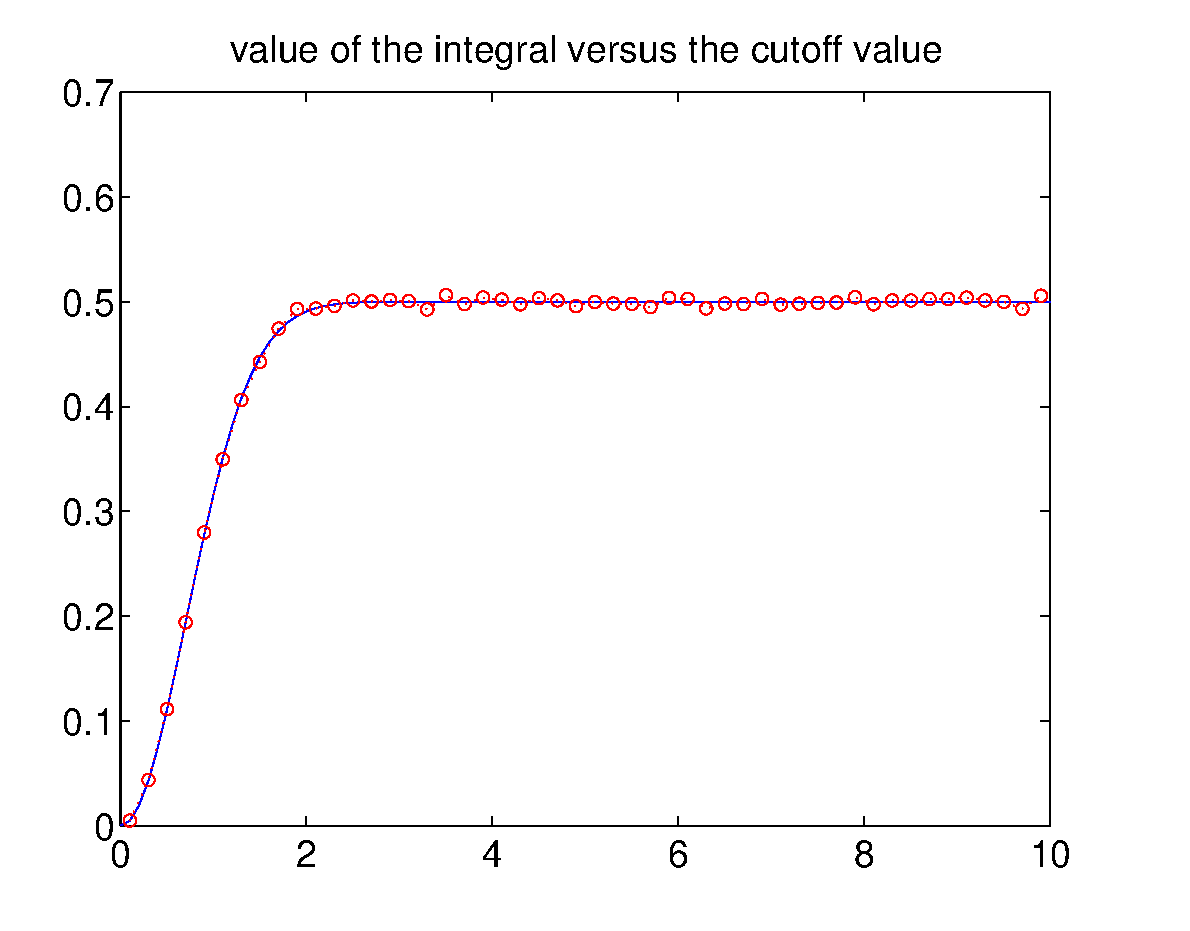
\includegraphics[width=0.47\textwidth]{f_importance_1.eps}\hfill
    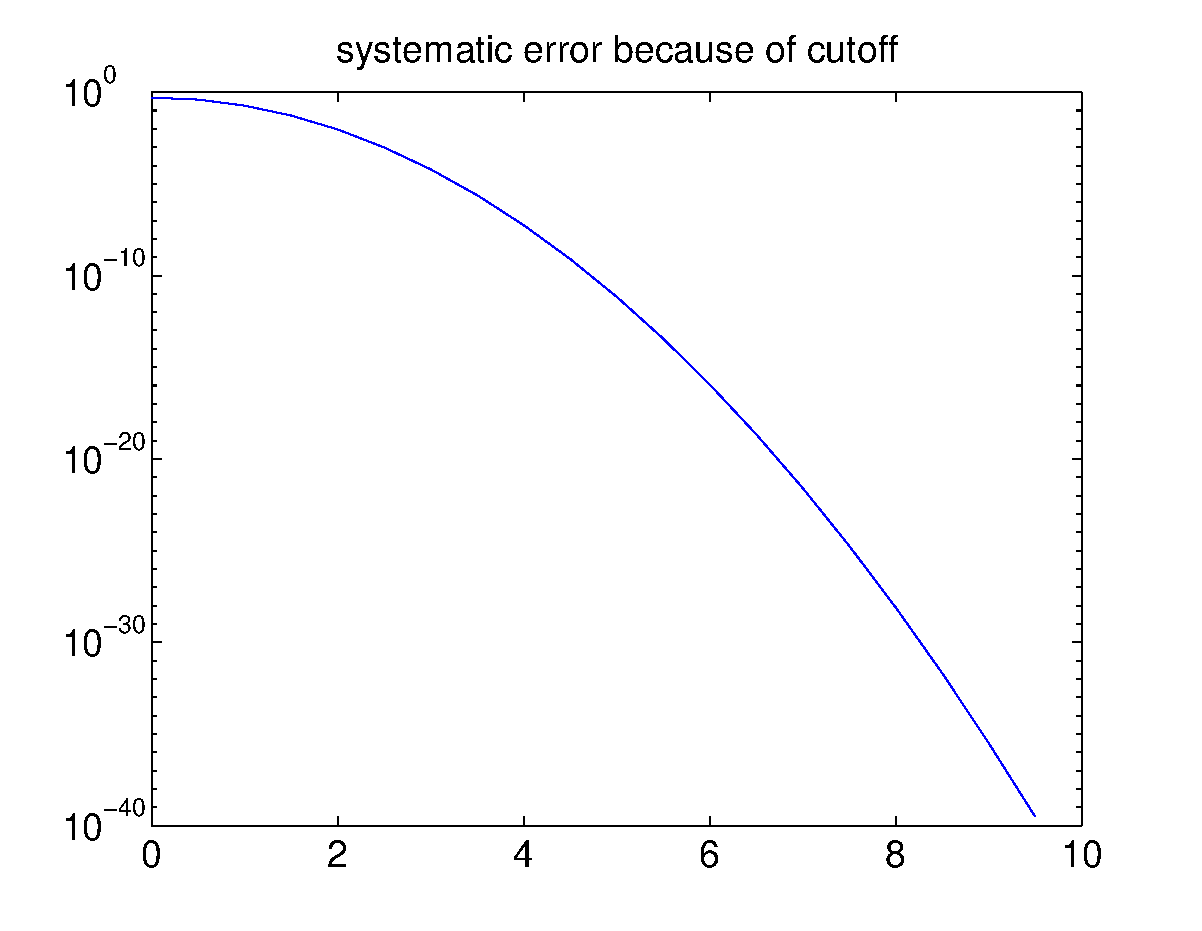
\includegraphics[width=0.47\textwidth]{f_importance_2.eps}
  \end{center}

  On the left I have plotted the function to be integrated. On the
  right there is again a result of a run using 1000 points:
  the blue line is the exact result, the red boxes are the
  importance sampling results and the black boxes are the simple
  sampling results.
  \begin{center}
    \includegraphics[width=0.47\textwidth]{f_importance_3.eps}\hfill
    \includegraphics[width=0.47\textwidth]{f_importance_4.eps}
  \end{center}

  {\bf short discussion about (exact) variance:}\\
  The variance of the importance sampling method can be analytically
  calculated for this case. The general formula is
  $$ \sigma^2 = \int_a^b \frac{g^2(x)}{f^2(x)} f(x) dx - \overline{I}^2,$$
  where
  $$ \overline{I} = \int_a^b \frac{g(x)}{f(x)} f(x) dx $$
  is the integral we are looking for (This is just the second moment
  minus the first moment squared, as usual.).

  In our case the first moment (the solution) is just $1/2$ for the interval
  $0$ to $\infty.$ For an interval from $0$ to $c$ we have
  $$ \int_0^c v e^{-v^2} dv = 1/2-{\frac {{e^{-c^{2}}}}{2}} .$$
  The second moment is just
  $$ \int_0^c v^2 e^{-d v^2} dv = -{\frac {2\,{e^{-dc^{2}}}d^{3/2}c-
      \sqrt{\pi }{\it erf}(\sqrt {d}c)d}{4\,d^{5/2}}} .$$
  (${\it erf}(c)$ is the error function.)

  With the help of the above formulas, we can discuss three possible
  sampling functions methods: \\
  {\bf -- we use as an example $c=10$ --}
  \begin{enumerate}
  \item the standard sampling using uniform deviates $f(x)=\frac{1}{(b-a)}=1/c$:\\
    $$ \sigma^2 = \int_0^c \frac{v^2 e^{-2v^2}}{1/c^2} \frac{1}{c} dv - %
          \frac{1}{4} =  1.316642671 .$$
  \item use  importance function $f(x)= \frac{1}{\sqrt{2\pi}}
       e^{-\frac{v^2}{2}}$:\\
    $$ \sigma^2 = \int_0^c \frac{v^2 e^{-2v^2}}{1/2\pi e^{-v^2}}
       \frac{1}{\sqrt{2\pi}}e^{-\frac{v^2}{2}} dv - \frac{1}{4}
       = 0.3545997878 .$$
  \item use importance function $f(x)=e^{-v^2}$:\\
    $$ \sigma^2 = \int_0^c \frac{v^2 e^{-2v^2}}{e^{-2v^2}} e^{-v^2} dv - %
      \frac{1}{4} =  0.1931134628 .$$
  \end{enumerate}
  As you can clearly see, the variance is greatly reduced by choosing an
  importance function very close to the function to be integrated.
  And of course the simple sampling Monte Carlo integration produces a
  big variance compared to the importance sampling method (here almost
  a factor of $4$ to $6$.).
\end{Solution}

\begin{Solution}{First_Passage_Times}
\textbf{First Passage Times (fpt) - \texttt{first\_passage.m}} \\
  The left figure shows a run using $R=5$ and 10.000 walks. The mean
  first passage time is $30,03$ steps.

  On the right, I have done many runs with different $R$ and calculated
  the mean first passage time for each run. You can see the exponential
  growth of the mean fpt.

  \begin{center}
    \includegraphics[width=0.47\textwidth]{f_firstpassage_1.eps}\hfill
    \includegraphics[width=0.47\textwidth]{f_firstpassage_2.eps}
  \end{center}
\end{Solution}

\begin{Solution}{Scaling_Random_Walk}
\textbf{Scaling Behavior of Random Walk in 2D and 3D - %
                 \texttt{rw\_scaling.m}} \\
The function to be fitted is:
$$ <R^2> = a N^b \quad .$$

For the plots below we used 100 realizations for each length $N.$
We started with length $50$ and the last length calculated was $2000 .$
  \begin{center}
    \hspace*{-1cm}
    \includegraphics[width=0.47\textwidth]{f_rw2dscaling.eps}\hfill
    \includegraphics[width=0.47\textwidth]{f_rw3dscaling.eps}
  \end{center} 
  Results of the 2D and 3D calculations:
  \begin{itemize}
  \item 2D scaling: $ a=1.1051$ and $b=0.9833 .$
  \item 3D scaling: $ a=0.9829$ and $b=1.0018 .$
  \end{itemize}

A second run was made, using 500 realizations for each length of
the random walk. We started with length $10$ and went up to length
$10,000$ (using 50 (in 3D) and 30 (in 2D) intermediate lengths). 
It took a total of $20,900$
seconds to calculate on a Pentium 200MMX processor (Matlab 5.0).
  \begin{center}
    \hspace*{-1cm}
    \includegraphics[width=0.47\textwidth]{f_rw3dscaling2.eps}\hfill
    \includegraphics[width=0.47\textwidth]{f_rw2dscaling2.eps}
  \end{center} 
  For the long runs, the results are:
  \begin{itemize}
  \item 2D scaling: $ a= 0.996679$ and $b= 1.001098 .$
  \item 3D scaling: $ a= 1.005113$ and $b= 0.999942 .$
  \end{itemize}
\end{Solution}

\begin{Solution}{Percolation}
\textbf{Percolation in 2D and Cluster Algorithms  - %
                      \texttt{percolation.m}}\\

The first two figures show $20\times 20$ configurations with and 
without a spanning
cluster. For the left figure we used $p=0.5$ and for the right figure
$p=0.55.$ 
  \begin{center}
    \hspace*{-1cm}
    \includegraphics[width=0.47\textwidth]{f_percolation_3.eps}\hfill
    \includegraphics[width=0.47\textwidth]{f_percolation_4.eps}
  \end{center} 

The following two figures are created using:
\begin{enumerate}
\item figure on the left: \\
  $N=20, p$ from $0.3$ to $0.9$ with stepsize $0.02$ and $20$ 
  realizations each.
\item figure on the right: \\
  $N=30, p$ from $0.3$ to $0.9$ with stepsize $0.02$ and $20$ 
  realizations each.
\end{enumerate}
  \begin{center}
    \hspace*{-1cm}
    \includegraphics[width=0.47\textwidth]{f_percolation_1.eps}\hfill
    \includegraphics[width=0.47\textwidth]{f_percolation_2.eps}
  \end{center} 

To estimate the critical probability $p_c$, you have to extract $p_c$
from the figures above. There are many ways of doing it. One would be
to fit a sigmoidal function 
$$p(x,a)=\left( \frac{1}{1+e^{-a(x-0.5)}}+1 \right) /2 ,$$ 
or a tangent hyperbolicus
$$ p(x,a)=(\tanh(a (x/2-0.5))+1)/2 = \left( 1+\frac{1-e^{-a(x-0.5)}}%
  {1+e^{-a(x-0.5)}} \right) /2 .$$
$a$ is the parameter to fit.
\end{Solution}

\begin{Solution}{Einstein_Solid}
\textbf{The Einstein Solid and the Boltzmann Distribution - %
                 \texttt{einstein\_solid.m}} \\

A typical 20x20 plane of the Einstein solid after 10000 jumps.
  \begin{center} 
   \begin{verbatim}
 1 2 0 0 0 3 5 2 0 1 1 1 0 0 1 1 2 0 1 0
 2 0 2 1 4 1 1 0 1 0 2 2 0 1 0 4 0 0 1 0
 3 1 3 0 1 0 1 0 0 0 0 0 0 1 1 1 0 1 0 1
 0 1 0 0 0 0 1 2 1 1 0 0 1 1 1 2 0 0 0 1
 0 0 6 1 0 4 0 0 1 1 1 0 0 0 0 0 0 0 0 2
 0 0 2 1 9 3 0 1 2 1 0 0 3 0 6 1 2 0 0 0
 0 2 2 1 0 2 0 0 0 0 0 2 4 0 0 0 0 0 1 1
 0 0 0 6 1 0 0 6 1 1 0 0 0 0 0 0 3 0 1 0
 2 0 1 0 0 2 0 1 0 2 0 0 0 1 3 0 0 1 0 3
 0 1 1 0 2 0 0 0 0 1 0 2 1 2 2 1 0 2 2 1
 1 0 2 0 1 1 2 0 0 0 4 1 1 3 0 0 2 0 4 1
 1 0 0 0 1 0 3 2 0 0 0 0 0 0 0 0 1 0 1 1
 0 2 2 0 1 3 0 2 1 2 1 0 0 1 2 0 0 2 2 3
 0 2 0 0 0 3 2 0 1 3 0 0 0 2 0 0 0 1 1 4
 2 0 0 0 0 5 0 3 0 0 0 1 0 0 0 2 2 2 1 2
 0 4 1 0 5 0 0 0 1 0 0 0 1 4 0 5 2 0 0 0
 1 0 1 2 0 0 0 0 2 0 0 5 0 1 2 1 0 2 0 0
 0 0 0 1 0 1 0 0 1 5 0 4 0 0 0 4 1 0 4 1
 0 1 0 3 4 0 1 2 1 5 0 3 9 0 0 1 0 3 0 2
 1 3 1 0 7 0 0 2 0 0 1 0 0 2 0 3 0 1 0 2
   \end{verbatim}
  \end{center}

On the next 9 figures you can see the time development of a 20x20
grid after 10, 20, 30, 40, 50, 60, 70, 150 and 20000 steps (or jumps).
Although it is a contour plot and not the whole cell is filled with
the same color (which would make it easier to view), you can still
see the pile up of quantas in individual cells. On the other side
more and more cells are unoccupied and after reaching equilibrium
we are left with most of the cells unoccupied.  

The last figure in this sequence is a semilogarithmic plot of the 
distribution of number of quantas in the cells (red curve). The blue
one is a least square fit to the Boltzmann distribution, which is in
excellent agreement. 
  \begin{center}
    \hspace*{-1cm}
    \includegraphics[width=0.47\textwidth]{f_einsteinsolid1.eps}\hfill
    \includegraphics[width=0.47\textwidth]{f_einsteinsolid2.eps}
  \end{center} 
  \begin{center}
    \hspace*{-1cm}
    \includegraphics[width=0.47\textwidth]{f_einsteinsolid3.eps}\hfill
    \includegraphics[width=0.47\textwidth]{f_einsteinsolid4.eps}
  \end{center} 
  \begin{center}
    \hspace*{-1cm}
    \includegraphics[width=0.47\textwidth]{f_einsteinsolid5.eps}\hfill
    \includegraphics[width=0.47\textwidth]{f_einsteinsolid6.eps}
  \end{center} 
  \begin{center}
    \hspace*{-1cm}
    \includegraphics[width=0.47\textwidth]{f_einsteinsolid7.eps}\hfill
    \includegraphics[width=0.47\textwidth]{f_einsteinsolid15.eps}
  \end{center} 
  \begin{center}
    \hspace*{-1cm}
    \includegraphics[width=0.47\textwidth]{f_einsteinsolid20.eps}\hfill
    \includegraphics[width=0.47\textwidth]{f_einsteinsolid40.eps}
  \end{center} 

As an example we have also done a caluclation with a 40x40 plane.
On the left is the filled contour plot and on the right is the same
configuration using a simple contour plot.
  \begin{center}
    \hspace*{-1cm}
    \includegraphics[width=0.47\textwidth]{f_einsteinsolid41.eps}\hfill
    \includegraphics[width=0.47\textwidth]{f_einsteinsolid42.eps}
  \end{center} 
\end{Solution}

%%%%%%%%%%%%%%%%%%%%%%%%%%%%%%%%%%%%%%%%%%%%%%%%%%%%%%%%%%%%%%%
\section{Solutions for Chapter 4}

\begin{Solution}{Linear_One_Step}
\textbf{ Linear one-step process - quantized harmonic oscillator in a %
    radiation field  - \texttt{onestepfast.m, qmharmoscimaster.m}}\\

{\small 
First of all we want to summarize some of the results for the one-step
processes (also called birth-and-death processes). They are goverend by the
following Master-equation (the phase space is discrete)
$$ \frac{\partial}{\partial t} P(n,t) = r(n)P(n-1,t)+g(n)P(n+1,t)
        -(r(n)+g(n))P(n,t) .$$
The solutions are continous in time, in contrast to the random walks 
discussed in the first few chapters. We can rewrite the Master-equation,
using the transition matrix 
$$\mathbb{W}_{nn'} := g_{n'}\delta_{n,n'-1} + r_{n'}\delta_{n,n'+1} \quad
   \text{for}\quad n\neq n' , \text{and} $$
$$\mathbb{W}_{nn} := -(r_n+g_n) \quad ,$$ 
as 
$$ \frac{\partial}{\partial t} P(n,t) = \mathbb{W}_{n,n'} P(n',t) .$$
There are three classes of one-step processes, depending on the interval
of $n$:
\begin{enumerate}
\item $(-\infty,+\infty)$, no limits on $n$.
\item $[0,+\infty)$, one sided open interval.
\item $(0,N)$, finite interval.
\end{enumerate}
We can take these boundary conditions into account by supplying
the correct equations for the boundaries, or in most cases it is
sufficient to just set e.g. $r(0)=0$ and $g(-1)=0$ or e.g. $r(N+1)=g(N)=0$.

The exact equation for the first moment is:
$$ \frac{\text{d}}{\text{d}t} <n> = -<r(n)> + <g(n)> , %
                     \quad \text{\textsc{first moment}} $$
and for the second moment
$$ \frac{\text{d}}{\text{d}t} <n^2> = 2<n(g(n)-r(n))> + <r(n)+g(n)> %
                     \quad \text{\textsc{second moment}}.$$
With these two solutions we can easily calculate the equation for the variance.

There are some interesting special cases, depending on the form of the
gain ($g(n)$) and the loss ($r(n)$) probability:
(RW stands for Random Walk)

\begin{center}
\begin{tabular}{c|c|c}
$g(n)$ & $r(n)$ & name \\\hline\hline
const.   &  $0$   & Poisson Process \\
$q=$const. &  $q=$const. & symmetric RW (diffusion) \\
$q_1=$const. & $q_2=$const. & asymmetric RW (diffusion with external force) \\
$0$        & $\gamma n$ & radioactive decay \\
$q=$const. & $k n$ & monomolecular chemical reaction \\
$\alpha n$ &  $\beta n$  & general linear (e.g. QM harm. osci., payroll) \\
higher orders in $n$ & higher orders in $n$ & nonlinear (e.g. competitive growth)\\
\end{tabular}
\end{center}
Remark: sometimes one refers to the nonlinearity of $g(n)$ and $r(n)$ by calling
it a nonlinear Master-equation, but do not forget that the Master-equation 
is always linear in $P(n,t)$! For the linear case, one must have at least one 
boundary, otherwise the transition probabilities $g(n)$ or $r(n)$ become negative. But
most of the physical systems have a {\em natural boundary}, like the radioactive decay
at $n=0$.

The stationary solution ($t\to\infty$) is given by:
$$ P_{\text{stat}}(n)= \frac{\prod\limits_{i=0}^{n-1}g(i)}{\prod\limits_{i=1}^{n}r(i)} P_{\text{stat}}(0)
      \quad \text{for}\quad n\geq 0 ,$$
and
$$ P_{\text{stat}}(n)=\frac{\prod\limits_{i=0}^{n+1}r(i)}{\prod\limits_{i=1}^{n}g(i)} P_{\text{stat}}(0)
      \quad \text{for}\quad n<0 .$$
The first solution is for the class 2 and 3 above and the second solution
is only for the class 1. $P_{\text{stat}}(0)$ is given by the normalization
condition, e.g. for class 2
$$ \sum_{i=0}^\infty P_{\text{stat}}(i) = 1 .$$

If we take the Fokker-Planck limit for the Random Walk (both transition rates
constant) we get a diffusion equation. The same limit for the Poisson process
(no loss transition) does not exist!  
}% End small

For the quantized harmonic oscillator we have for the first moment 
(The initial condition will be always $n(0)=N_0.)$
$$ \frac{\text{d}}{\text{d}t} <n> = (\beta-\alpha) <n> \quad \Rightarrow %
   \quad  <n(t)>= N_0 e^{ (\beta-\alpha) t} \quad\text{and}$$
$$ \frac{\text{d}}{\text{d}t} <n^2> = 2(\beta-\alpha)<n^2>+(\alpha+\beta)<n>,$$
which has the solution 
$$ <n^2(t)> = \frac{\alpha+\beta}{\alpha-\beta}N_0 e^{ (\beta-\alpha) t} %
  \left(1-e^{ (\beta-\alpha) t}\right)+N_0^2 e^{2(\beta-\alpha) t} .$$
(Remark: As you can see, we have a closed hierachy of moment equations.)

The stationary solution is
$$  P_{\text{stat}}(n)= \text{const.} \,\cdot \left(\frac{\beta}{\alpha}\right)^n .$$

\hrule
Here are some results of the simulation:
\begin{itemize}
\item \mathversion{bold}$\alpha=\beta=0.5,$ \mathversion{normal}%
           $N_0=50, t_{\text{END}}=500, 1$ realization$, \Delta t=1$ 
  \begin{center}
    \hspace*{-1cm}
    \includegraphics[width=0.47\textwidth]{f_qmharmosci_1.eps}\hfill
    \includegraphics[width=0.47\textwidth]{f_qmharmosci_2.eps}
  \end{center} 
\item \mathversion{bold}$\alpha=\beta=0.5,$ \mathversion{normal}%
           $N_0=50, t_{\text{END}}=100, 100$ realizations$, \Delta t=2$ 
  \begin{center}
    \hspace*{-1cm}
    \includegraphics[width=0.3\textwidth]{f_qmharmosci_3.eps}\hfill
    \includegraphics[width=0.3\textwidth]{f_qmharmosci_4.eps}\hfill
    \includegraphics[width=0.3\textwidth]{f_qmharmosci_5.eps}
  \end{center} 
\item \mathversion{bold}$\alpha=0.52, \beta=0.48,$ \mathversion{normal}%
           $N_0=500, t_{\text{END}}=150, 1$ realization$, \Delta t=1$ 
  \begin{center}
    \hspace*{-1cm}
    \includegraphics[width=0.47\textwidth]{f_qmharmosci_6.eps}\hfill
    \includegraphics[width=0.47\textwidth]{f_qmharmosci_7.eps}
  \end{center} 
\item \mathversion{bold}$\alpha=0.51, \beta=0.49,$ \mathversion{normal}%
           $N_0=50, t_{\text{END}}=100, 100$ realizations$, \Delta t=2$ 
  \begin{center}
    \hspace*{-1cm}
    \includegraphics[width=0.3\textwidth]{f_qmharmosci_8.eps}\hfill
    \includegraphics[width=0.3\textwidth]{f_qmharmosci_9.eps}\hfill
    \includegraphics[width=0.3\textwidth]{f_qmharmosci_10.eps}
  \end{center} 
\item \mathversion{bold}$\alpha=0.53, \beta=0.47,$ \mathversion{normal}%
           $N_0=50, t_{\text{END}}=50, 300$ realizations$, \Delta t=1$ 
  \begin{center}
    \hspace*{-1cm}
    \includegraphics[width=0.3\textwidth]{f_qmharmosci_11.eps}\hfill
    \includegraphics[width=0.3\textwidth]{f_qmharmosci_12.eps}\hfill
    \includegraphics[width=0.3\textwidth]{f_qmharmosci_13.eps}
  \end{center} 
  \begin{center}
    \hspace*{-1cm}
    \includegraphics[width=0.3\textwidth]{f_qmharmosci_14.eps}\hfill
    \includegraphics[width=0.3\textwidth]{f_qmharmosci_15.eps}\hfill
    \includegraphics[width=0.3\textwidth]{f_qmharmosci_16.eps}
  \end{center} 
\item \mathversion{bold}$\alpha=0.50, \beta=0.51,$ \mathversion{normal}%
           $N_0=10, t_{\text{END}}=50, 200$ realizations$, \Delta t=1$ 
  \begin{center}
    \hspace*{-1cm}
    \includegraphics[width=0.3\textwidth]{f_qmharmosci_17.eps}\hfill
    \includegraphics[width=0.3\textwidth]{f_qmharmosci_18.eps}\hfill
    \includegraphics[width=0.3\textwidth]{f_qmharmosci_19.eps}
  \end{center} 
  \begin{center}
    \hspace*{-1cm}
    \includegraphics[width=0.47\textwidth]{f_qmharmosci_20.eps}\hfill
    \includegraphics[width=0.47\textwidth]{f_qmharmosci_21.eps}
  \end{center} 
\end{itemize}
\end{Solution}

\begin{Solution}{Nonlinear_One_Step}
\textbf{ Non-linear one-step process - growth of a competitive %
    population - \texttt{onestepfast.m, nonlingrowthmaster.m}} \\
This time the transition rates are $r(n)= \beta n$ and 
$g(n)=\alpha n + \gamma n(n-1)$. The solutions for the first moment are 
$$ <n(t)>=\frac{\beta-\alpha}{\gamma} \quad\text{and}\quad <n(t)>\equiv 0 .$$

Here are some examples of the simulation:
\begin{itemize}
\item LEFT: 
        \mathversion{bold}$\alpha=0.50, \beta=1.0, \gamma=0.05$ \mathversion{normal}%
           $N_0=100, t_{\text{END}}=500, 1$ realization$, \Delta t=2$ and \\
RIGHT: 
\mathversion{bold}$\alpha=0.1, \beta=1.1, \gamma=0.01$ \mathversion{normal}%
           $N_0=120, t_{\text{END}}=30, 1$ realization$, \Delta t=1$
  \begin{center}
    \hspace*{-1cm}
    \includegraphics[width=0.45\textwidth]{f_nonlingrowth_1.eps}\hfill
    \includegraphics[width=0.45\textwidth]{f_nonlingrowth_2.eps}
  \end{center} 
\item \mathversion{bold}$\alpha=0.1, \beta=1.1, \gamma=0.01$ \mathversion{normal}%
           $N_0=120, t_{\text{END}}=10, 100$ realizations$, \Delta t=1$ 
  \begin{center}
    \hspace*{-1cm}
    \includegraphics[width=0.45\textwidth]{f_nonlingrowth_4.eps}\hfill
    \includegraphics[width=0.45\textwidth]{f_nonlingrowth_5.eps}
  \end{center} 
  \begin{center}
    \hspace*{-1cm}
    \includegraphics[width=0.45\textwidth]{f_nonlingrowth_3.eps}\hfill
    \includegraphics[width=0.45\textwidth]{f_nonlingrowth_6.eps}
  \end{center} 

\end{itemize}
\end{Solution}

\begin{Solution}{Random_Telegraph}
\textbf{ The Random Telegraph Process  - \texttt{onestepfast.m, telegraphmaster.m}}\\

First of all you have to rewrite the master-equation into the known
form. Therefore you have to identify the transition rates as
$$ r(n)=a n \quad\text{and}\quad g(n)=b(1-n) .$$


Some analytical results:
$$ <n(t)> = <n^2(t)> =\frac{a}{a+b} ,$$

Here are some results of the simulation:
\begin{itemize}
\item %
LEFT: \mathversion{bold}$a=0.1, b=0.9,$ \mathversion{normal}%
           $N_0=1, t_{\text{END}}=10, 1$ realization$, \Delta t=1$ and \\ 
RIGHT: \mathversion{bold}$a=0.1, b=0.9,$ \mathversion{normal}%
           $N_0=1, t_{\text{END}}=100, 1$ realization$, \Delta t=1$
  \begin{center}
    \hspace*{-1cm}
    \includegraphics[width=0.47\textwidth]{f_telegraph_1.eps}\hfill
    \includegraphics[width=0.47\textwidth]{f_telegraph_2.eps}
  \end{center} 
\item \mathversion{bold}$a=0.1, b=0.9,$ \mathversion{normal}%
           $N_0=1, t_{\text{END}}=50, 100$ realizations$, \Delta t=1$ \\
You can see that the first and the second moment have the same value, like
expected by the analytical results. The probability distribution in
the last figure shows $P(0)$ and $P(1)$.
  \begin{center}
    \hspace*{-1cm}
    \includegraphics[width=0.47\textwidth]{f_telegraph_3.eps}\hfill
    \includegraphics[width=0.47\textwidth]{f_telegraph_5.eps}
  \end{center} 
  \begin{center}
    \hspace*{-1cm}
    \includegraphics[width=0.47\textwidth]{f_telegraph_4.eps}\hfill
    \includegraphics[width=0.47\textwidth]{f_telegraph_6.eps}
  \end{center} 
\item \mathversion{bold}$a=0.1, b=0.9,$ \mathversion{normal}%
           $N_0=1, t_{\text{END}}=10, 100$ realizations$, \Delta t=0.2$ \\
The left figure shows a patch plot of the correlation matrix. The colorbar
identifies the colors with the corresponding values of the correlation matrix.
The red line indicates the normalized second moment $<n(t)n(t)>=<n^2(t)>.$
The right figure displays five correlation functions with a fixed $t$ and
varying time difference $t-t'$. As expected the correlation decays 
exponentially and the correlation length i about $1/(a+b)$ (see asssignment).
  \begin{center}
    \hspace*{-1cm}
    \includegraphics[width=0.47\textwidth]{f_telegraph_7.eps}\hfill
    \includegraphics[width=0.47\textwidth]{f_telegraph_8.eps}
  \end{center} 

\end{itemize}
\end{Solution}

%%%%%%%%%%%%%%%%%%%%%%%%%%%%%%%%%%%%%%%%%%%%%%%%%%%%%%%%%%%%%%%%%%%%

\begin{Solution}{Monomolecular_Reaction}
\textbf{ Monomolecular Chemical Reaction $A \leftrightarrows X$  %
    - \texttt{onestepfast.m, reactionmaster.m}} \\
First of all let us calculate the stationary distribution here as an example.
$$ P_{\text{stat}}(n)= \frac{\prod\limits_{i=0}^{n-1}g(i)}{\prod\limits_{i=1}^{n}
        r(i)} P_{\text{stat}}(0) = \frac{A^n}{n! k^n} P_{\text{stat}}(0) ,$$
and 
\begin{eqnarray*}
 \sum_{i=0}^\infty P_{\text{stat}}(i) &=& P_{\text{stat}}(0) + 
        \sum_{i=1}^\infty P_{\text{stat}}(i) = P_{\text{stat}}(0) +
        \sum_{i=1}^\infty \frac{A^i}{i! k^i} P_{\text{stat}}(0) = \\
&=& P_{\text{stat}}(0) \left( 1+ (e^{Ak}-1)\right) = P_{\text{stat}}(0)e^{Ak}, 
\end{eqnarray*}
and therefore
$$ P_{\text{stat}}(0) = e^{-Ak} \quad\Rightarrow\quad P_{\text{stat}}(n)=
        \frac{A^n}{n!} e^{-Ak} .$$
The rest of the analytical results are given in the assignment, we don not repeat 
them here.


Here are some examples of the simulation:
\begin{itemize}
\item \mathversion{bold}$k=1, A=100,$ \mathversion{normal}%
           $N_0=100, t_{\text{END}}=80, 1$ realization
  \begin{center}
    \includegraphics[width=0.5\textwidth]{f_reaction_1.eps}
  \end{center} 
\item \mathversion{bold}$k=1, A=100,$ \mathversion{normal}%
           $N_0=100, t_{\text{END}}=50, 100$ realizations$, \Delta t=1$ 
  \begin{center}        
    \hspace*{-1cm}
    \includegraphics[width=0.45\textwidth]{f_reaction_2.eps}\hfill
    \includegraphics[width=0.45\textwidth]{f_reaction_3.eps}
  \end{center} 
  \begin{center}        
    \hspace*{-1cm}
    \includegraphics[width=0.45\textwidth]{f_reaction_4.eps}\hfill
    \includegraphics[width=0.45\textwidth]{f_reaction_5.eps}
  \end{center} 
The red line in the right figure is a Poisson distribution (which is
the analytical result for the stationary distribution for this process.)
with mean $100$. You can see the excellent agreement with the simulated curve.

\end{itemize}
\end{Solution}

%%%%%%%%%%%%%%%%%%%%%%%%%%%%%%%%%%%%%%%%%%%%%%%%%%%%%%%%%%%%%%%
\section{Solutions for Chapter 5}
\begin{Solution}{Johnson_Noise}
\textbf{Johnson Noise - \texttt{sdeornstein.m}} \\

First of all you have to identify the parameters (functions) $q$ and $D$
of the SDE form used in the lecture:
$$ q= 1/\tau, \quad \text{and}\quad D=c .$$

Some simulation results:     
\begin{itemize}
\item \mathversion{bold}$i_0=0, q=1, D=1,$ \mathversion{normal}%
           $t_{\text{END}}=1000, \Delta t=0.2, 1000$ realizations\\
The last figure on the right is a simulation for different time
discretizations $\Delta t=0.5, 0.2$ and $0.1$ using $2000$ realizations
and $t_{\text{END}}=100$.
  \begin{center}
    \hspace*{-1cm}
    \includegraphics[width=0.47\textwidth]{f_johnson_2.eps}\hfill
    \includegraphics[width=0.47\textwidth]{f_johnson_3.eps}
  \end{center}
  \begin{center}
    \hspace*{-1cm}
    \includegraphics[width=0.47\textwidth]{f_johnson_1.eps}\hfill
    \includegraphics[width=0.47\textwidth]{f_johnson_4.eps}
  \end{center}
\newpage
\item \mathversion{bold}$i_0=0, q=0.01, D=100,$ \mathversion{normal}%
           $t_{\text{END}}=250, \Delta t=0.2, 100$ realizations
  \begin{center}
    \hspace*{-1cm}
    \includegraphics[width=0.47\textwidth]{f_johnson_5.eps}\hfill
    \includegraphics[width=0.47\textwidth]{f_johnson_6.eps}
  \end{center}
  \begin{center}
    \hspace*{-1cm}
    \includegraphics[width=0.6\textwidth]{f_johnson_7.eps}
  \end{center}
\end{itemize}
\end{Solution}

%%%%%%%%%%%%%%%%%%%%%%%%%%%%%%%%%%%%%%%%%%%%%%%%%%%%%%%%%%%%%%%
\section{Solutions for Chapter 6}
\begin{Solution}{xxx}
\end{Solution}
%%%%%%%%%%%%%%%%%%%%%%%%%%%%%%%%%%%%%%%%%%%%%%%%%%%%%%%%%%%%%%%
\section{Solutions for Chapter 7}

%%%%%%%%%%%%%%%%%%%%%%%%%%%%%%%%%%%%%%%%%%%%%%%%%%%%

\bibliographystyle{peter}
\bibliography{V_98,simulit}


%%%%%%%%%%%%%%%%%%%%%%%%%%%%%%%%%%%%%%%%%%%%%%%%%%%%



% Bibliographien
%% These commands are ignored by the chapterbib package
%%\bibliographystyle{peter}
%%\bibliography{V_98,simulit}

%%\addtocontents{toc}{\protect\vspace{1.5ex}}
%%\addcontentsline{toc}{chapter}{\protect\numberline{}Bibliography}
%%\clearpage

% Now insert the Index
%%\addtocontents{toc}{\protect\vspace{1.5ex}}
%%\addcontentsline{toc}{chapter}{\protect\numberline{}Index}
%%\printindex

\end{document}
